% Created by tikzDevice version 0.8.1 on 2015-01-10 20:43:00
% !TEX encoding = UTF-8 Unicode
% Calculated character metrics. ascent: 8.264620, descent: 0.000000, width: 10.997280
% Calculated string width of 0.00 as 17.062600
% Calculated character metrics. ascent: 6.611760, descent: 0.000000, width: 8.797910
% Calculated string width of 0.25 as 17.062600
% Calculated string width of 0.50 as 17.062600
% Calculated string width of 0.75 as 17.062600
% Calculated string width of 1.00 as 17.062600
% Calculated character metrics. ascent: 8.264620, descent: 0.000000, width: 10.997280
% Calculated string width of 0.00 as 17.062600
% Calculated character metrics. ascent: 6.611760, descent: 0.000000, width: 8.797910
% Calculated string width of 0.25 as 17.062600
% Calculated string width of 0.50 as 17.062600
% Calculated string width of 0.75 as 17.062600
% Calculated string width of 1.00 as 17.062600
% Calculated character metrics. ascent: 8.264620, descent: 0.000000, width: 10.997280
% Drawing Rectangle from x0 = 0.000000, y0 = 0.000000 to x1 = 505.890000, y1 = 216.810000
% Beginning new tikzpicture 'page'
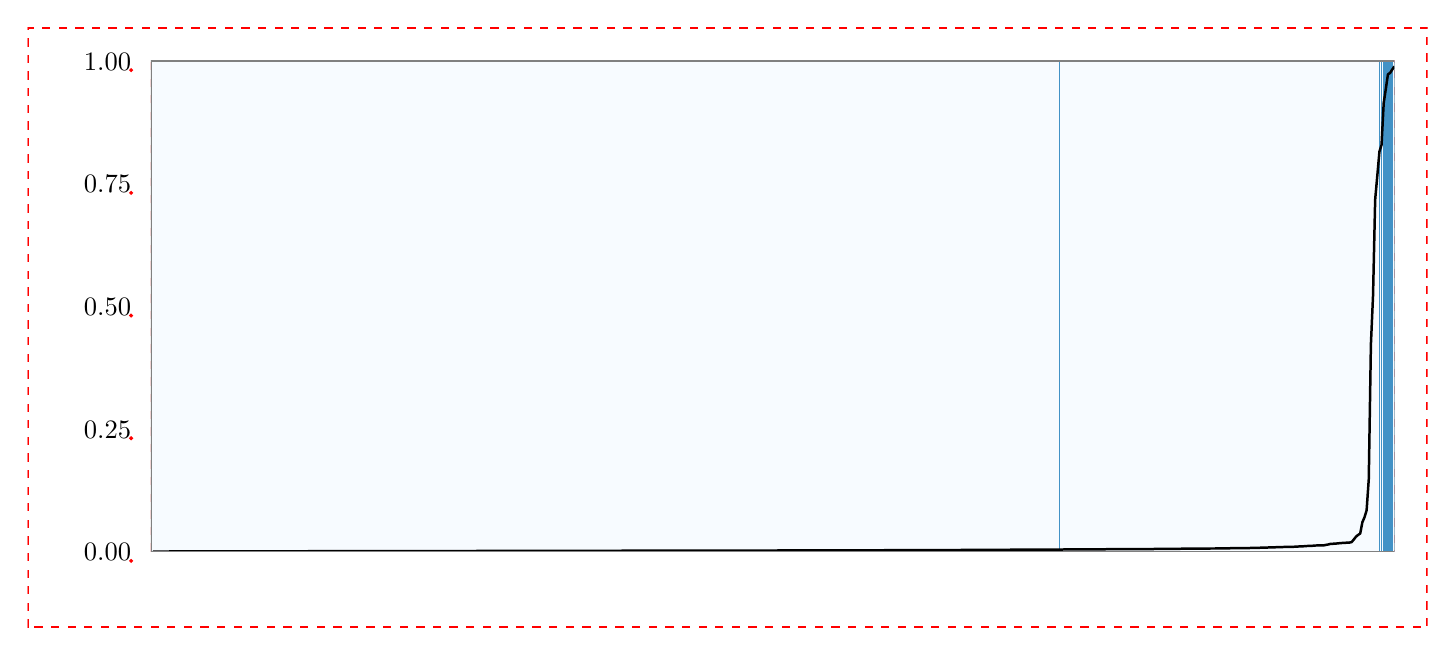
\begin{tikzpicture}[x=1pt,y=1pt]
\definecolor{fillColor}{RGB}{255,255,255}
\path[use as bounding box,fill=fillColor,fill opacity=0.00] (0,0) rectangle (505.89,216.81);
\begin{scope}
\path[clip] (  0.00,  0.00) rectangle (505.89,216.81);
\path[draw=red,very thick,dashed] (  0.00,  0.00) rectangle (505.89,216.81);
\definecolor{drawColor}{RGB}{255,255,255}
\definecolor{fillColor}{RGB}{255,255,255}

\path[draw=drawColor,line width= 0.6pt,line join=round,line cap=round,fill=fillColor] (  0.00,  0.00) rectangle (505.89,216.81);
\end{scope}
% Drawing Rectangle from x0 = 44.485409, y0 = 27.422809 to x1 = 493.845000, y1 = 204.765000
\begin{scope}
\path[clip] ( 44.49, 27.42) rectangle (493.85,204.77);
\path[draw=red,very thick,dashed] ( 44.49, 27.42) rectangle (493.85,204.77);
\definecolor{fillColor}{RGB}{247,251,255}

\path[fill=fillColor] ( 44.49, 27.42) rectangle (493.85,204.76);
% Drawing Rectangle from x0 = 44.485409, y0 = 27.422809 to x1 = 493.845000, y1 = 204.765000

\path[fill=fillColor] ( 44.49, 27.42) rectangle (493.85,204.76);
% Drawing Rectangle from x0 = 44.485409, y0 = 27.422809 to x1 = 493.845000, y1 = 204.765000

\path[fill=fillColor] ( 44.49, 27.42) rectangle (493.85,204.76);
% Drawing Rectangle from x0 = 44.485409, y0 = 27.422809 to x1 = 493.845000, y1 = 204.765000

\path[fill=fillColor] ( 44.49, 27.42) rectangle (493.85,204.76);
% Drawing Rectangle from x0 = 44.485409, y0 = 27.422809 to x1 = 493.845000, y1 = 204.765000

\path[fill=fillColor] ( 44.49, 27.42) rectangle (493.85,204.76);
% Drawing Rectangle from x0 = 44.485409, y0 = 27.422809 to x1 = 493.845000, y1 = 204.765000

\path[fill=fillColor] ( 44.49, 27.42) rectangle (493.85,204.76);
% Drawing Rectangle from x0 = 44.485409, y0 = 27.422809 to x1 = 493.845000, y1 = 204.765000

\path[fill=fillColor] ( 44.49, 27.42) rectangle (493.85,204.76);
% Drawing Rectangle from x0 = 44.485409, y0 = 27.422809 to x1 = 493.845000, y1 = 204.765000

\path[fill=fillColor] ( 44.49, 27.42) rectangle (493.85,204.76);
% Drawing Rectangle from x0 = 44.485409, y0 = 27.422809 to x1 = 493.845000, y1 = 204.765000

\path[fill=fillColor] ( 44.49, 27.42) rectangle (493.85,204.76);
% Drawing Rectangle from x0 = 44.485409, y0 = 27.422809 to x1 = 493.845000, y1 = 204.765000

\path[fill=fillColor] ( 44.49, 27.42) rectangle (493.85,204.76);
% Drawing Rectangle from x0 = 44.485409, y0 = 27.422809 to x1 = 493.845000, y1 = 204.765000

\path[fill=fillColor] ( 44.49, 27.42) rectangle (493.85,204.76);
% Drawing Rectangle from x0 = 44.485409, y0 = 27.422809 to x1 = 493.845000, y1 = 204.765000

\path[fill=fillColor] ( 44.49, 27.42) rectangle (493.85,204.76);
% Drawing Rectangle from x0 = 44.485409, y0 = 27.422809 to x1 = 493.845000, y1 = 204.765000

\path[fill=fillColor] ( 44.49, 27.42) rectangle (493.85,204.76);
% Drawing Rectangle from x0 = 44.485409, y0 = 27.422809 to x1 = 493.845000, y1 = 204.765000

\path[fill=fillColor] ( 44.49, 27.42) rectangle (493.85,204.76);
% Drawing Rectangle from x0 = 44.485409, y0 = 27.422809 to x1 = 493.845000, y1 = 204.765000

\path[fill=fillColor] ( 44.49, 27.42) rectangle (493.85,204.76);
% Drawing Rectangle from x0 = 44.485409, y0 = 27.422809 to x1 = 493.845000, y1 = 204.765000

\path[fill=fillColor] ( 44.49, 27.42) rectangle (493.85,204.76);
% Drawing Rectangle from x0 = 44.485409, y0 = 27.422809 to x1 = 493.845000, y1 = 204.765000

\path[fill=fillColor] ( 44.49, 27.42) rectangle (493.85,204.76);
% Drawing Rectangle from x0 = 44.485409, y0 = 27.422809 to x1 = 493.845000, y1 = 204.765000

\path[fill=fillColor] ( 44.49, 27.42) rectangle (493.85,204.76);
% Drawing Rectangle from x0 = 44.485409, y0 = 27.422809 to x1 = 493.845000, y1 = 204.765000

\path[fill=fillColor] ( 44.49, 27.42) rectangle (493.85,204.76);
% Drawing Rectangle from x0 = 44.485409, y0 = 27.422809 to x1 = 493.845000, y1 = 204.765000

\path[fill=fillColor] ( 44.49, 27.42) rectangle (493.85,204.76);
% Drawing Rectangle from x0 = 44.485409, y0 = 27.422809 to x1 = 493.845000, y1 = 204.765000

\path[fill=fillColor] ( 44.49, 27.42) rectangle (493.85,204.76);
% Drawing Rectangle from x0 = 44.485409, y0 = 27.422809 to x1 = 493.845000, y1 = 204.765000

\path[fill=fillColor] ( 44.49, 27.42) rectangle (493.85,204.76);
% Drawing Rectangle from x0 = 44.485409, y0 = 27.422809 to x1 = 493.845000, y1 = 204.765000

\path[fill=fillColor] ( 44.49, 27.42) rectangle (493.85,204.76);
% Drawing Rectangle from x0 = 44.485409, y0 = 27.422809 to x1 = 493.845000, y1 = 204.765000

\path[fill=fillColor] ( 44.49, 27.42) rectangle (493.85,204.76);
% Drawing Rectangle from x0 = 44.485409, y0 = 27.422809 to x1 = 493.845000, y1 = 204.765000

\path[fill=fillColor] ( 44.49, 27.42) rectangle (493.85,204.76);
% Drawing Rectangle from x0 = 44.485409, y0 = 27.422809 to x1 = 493.845000, y1 = 204.765000

\path[fill=fillColor] ( 44.49, 27.42) rectangle (493.85,204.76);
% Drawing Rectangle from x0 = 44.485409, y0 = 27.422809 to x1 = 493.845000, y1 = 204.765000

\path[fill=fillColor] ( 44.49, 27.42) rectangle (493.85,204.76);
% Drawing Rectangle from x0 = 44.485409, y0 = 27.422809 to x1 = 493.845000, y1 = 204.765000

\path[fill=fillColor] ( 44.49, 27.42) rectangle (493.85,204.76);
% Drawing Rectangle from x0 = 44.485409, y0 = 27.422809 to x1 = 493.845000, y1 = 204.765000

\path[fill=fillColor] ( 44.49, 27.42) rectangle (493.85,204.76);
% Drawing Rectangle from x0 = 44.485409, y0 = 27.422809 to x1 = 493.845000, y1 = 204.765000

\path[fill=fillColor] ( 44.49, 27.42) rectangle (493.85,204.76);
% Drawing Rectangle from x0 = 44.485409, y0 = 27.422809 to x1 = 493.845000, y1 = 204.765000

\path[fill=fillColor] ( 44.49, 27.42) rectangle (493.85,204.76);
% Drawing Rectangle from x0 = 44.485409, y0 = 27.422809 to x1 = 493.845000, y1 = 204.765000

\path[fill=fillColor] ( 44.49, 27.42) rectangle (493.85,204.76);
% Drawing Rectangle from x0 = 44.485409, y0 = 27.422809 to x1 = 493.845000, y1 = 204.765000

\path[fill=fillColor] ( 44.49, 27.42) rectangle (493.85,204.76);
% Drawing Rectangle from x0 = 44.485409, y0 = 27.422809 to x1 = 493.845000, y1 = 204.765000

\path[fill=fillColor] ( 44.49, 27.42) rectangle (493.85,204.76);
% Drawing Rectangle from x0 = 44.485409, y0 = 27.422809 to x1 = 493.845000, y1 = 204.765000

\path[fill=fillColor] ( 44.49, 27.42) rectangle (493.85,204.76);
% Drawing Rectangle from x0 = 44.485409, y0 = 27.422809 to x1 = 493.845000, y1 = 204.765000

\path[fill=fillColor] ( 44.49, 27.42) rectangle (493.85,204.76);
% Drawing Rectangle from x0 = 44.485409, y0 = 27.422809 to x1 = 493.845000, y1 = 204.765000

\path[fill=fillColor] ( 44.49, 27.42) rectangle (493.85,204.76);
% Drawing Rectangle from x0 = 44.485409, y0 = 27.422809 to x1 = 493.845000, y1 = 204.765000

\path[fill=fillColor] ( 44.49, 27.42) rectangle (493.85,204.76);
% Drawing Rectangle from x0 = 44.485409, y0 = 27.422809 to x1 = 493.845000, y1 = 204.765000

\path[fill=fillColor] ( 44.49, 27.42) rectangle (493.85,204.76);
% Drawing Rectangle from x0 = 44.485409, y0 = 27.422809 to x1 = 493.845000, y1 = 204.765000

\path[fill=fillColor] ( 44.49, 27.42) rectangle (493.85,204.76);
% Drawing Rectangle from x0 = 44.485409, y0 = 27.422809 to x1 = 493.845000, y1 = 204.765000

\path[fill=fillColor] ( 44.49, 27.42) rectangle (493.85,204.76);
% Drawing Rectangle from x0 = 44.485409, y0 = 27.422809 to x1 = 493.845000, y1 = 204.765000

\path[fill=fillColor] ( 44.49, 27.42) rectangle (493.85,204.76);
% Drawing Rectangle from x0 = 44.485409, y0 = 27.422809 to x1 = 493.845000, y1 = 204.765000

\path[fill=fillColor] ( 44.49, 27.42) rectangle (493.85,204.76);
% Drawing Rectangle from x0 = 44.485409, y0 = 27.422809 to x1 = 493.845000, y1 = 204.765000

\path[fill=fillColor] ( 44.49, 27.42) rectangle (493.85,204.76);
% Drawing Rectangle from x0 = 44.485409, y0 = 27.422809 to x1 = 493.845000, y1 = 204.765000

\path[fill=fillColor] ( 44.49, 27.42) rectangle (493.85,204.76);
% Drawing Rectangle from x0 = 44.485409, y0 = 27.422809 to x1 = 493.845000, y1 = 204.765000

\path[fill=fillColor] ( 44.49, 27.42) rectangle (493.85,204.76);
% Drawing Rectangle from x0 = 44.485409, y0 = 27.422809 to x1 = 493.845000, y1 = 204.765000

\path[fill=fillColor] ( 44.49, 27.42) rectangle (493.85,204.76);
% Drawing Rectangle from x0 = 44.485409, y0 = 27.422809 to x1 = 493.845000, y1 = 204.765000

\path[fill=fillColor] ( 44.49, 27.42) rectangle (493.85,204.76);
% Drawing Rectangle from x0 = 44.485409, y0 = 27.422809 to x1 = 493.845000, y1 = 204.765000

\path[fill=fillColor] ( 44.49, 27.42) rectangle (493.85,204.76);
% Drawing Rectangle from x0 = 44.485409, y0 = 27.422809 to x1 = 493.845000, y1 = 204.765000

\path[fill=fillColor] ( 44.49, 27.42) rectangle (493.85,204.76);
% Drawing Rectangle from x0 = 44.485409, y0 = 27.422809 to x1 = 493.845000, y1 = 204.765000

\path[fill=fillColor] ( 44.49, 27.42) rectangle (493.85,204.76);
% Drawing Rectangle from x0 = 44.485409, y0 = 27.422809 to x1 = 493.845000, y1 = 204.765000

\path[fill=fillColor] ( 44.49, 27.42) rectangle (493.85,204.76);
% Drawing Rectangle from x0 = 44.485409, y0 = 27.422809 to x1 = 493.845000, y1 = 204.765000

\path[fill=fillColor] ( 44.49, 27.42) rectangle (493.85,204.76);
% Drawing Rectangle from x0 = 44.485409, y0 = 27.422809 to x1 = 493.845000, y1 = 204.765000

\path[fill=fillColor] ( 44.49, 27.42) rectangle (493.85,204.76);
% Drawing Rectangle from x0 = 44.485409, y0 = 27.422809 to x1 = 493.845000, y1 = 204.765000

\path[fill=fillColor] ( 44.49, 27.42) rectangle (493.85,204.76);
% Drawing Rectangle from x0 = 44.485409, y0 = 27.422809 to x1 = 493.845000, y1 = 204.765000

\path[fill=fillColor] ( 44.49, 27.42) rectangle (493.85,204.76);
% Drawing Rectangle from x0 = 44.485409, y0 = 27.422809 to x1 = 493.845000, y1 = 204.765000

\path[fill=fillColor] ( 44.49, 27.42) rectangle (493.85,204.76);
% Drawing Rectangle from x0 = 44.485409, y0 = 27.422809 to x1 = 493.845000, y1 = 204.765000

\path[fill=fillColor] ( 44.49, 27.42) rectangle (493.85,204.76);
% Drawing Rectangle from x0 = 44.485409, y0 = 27.422809 to x1 = 493.845000, y1 = 204.765000

\path[fill=fillColor] ( 44.49, 27.42) rectangle (493.85,204.76);
% Drawing Rectangle from x0 = 44.485409, y0 = 27.422809 to x1 = 493.845000, y1 = 204.765000

\path[fill=fillColor] ( 44.49, 27.42) rectangle (493.85,204.76);
% Drawing Rectangle from x0 = 44.485409, y0 = 27.422809 to x1 = 493.845000, y1 = 204.765000

\path[fill=fillColor] ( 44.49, 27.42) rectangle (493.85,204.76);
% Drawing Rectangle from x0 = 44.485409, y0 = 27.422809 to x1 = 493.845000, y1 = 204.765000

\path[fill=fillColor] ( 44.49, 27.42) rectangle (493.85,204.76);
% Drawing Rectangle from x0 = 44.485409, y0 = 27.422809 to x1 = 493.845000, y1 = 204.765000

\path[fill=fillColor] ( 44.49, 27.42) rectangle (493.85,204.76);
% Drawing Rectangle from x0 = 44.485409, y0 = 27.422809 to x1 = 493.845000, y1 = 204.765000

\path[fill=fillColor] ( 44.49, 27.42) rectangle (493.85,204.76);
% Drawing Rectangle from x0 = 44.485409, y0 = 27.422809 to x1 = 493.845000, y1 = 204.765000

\path[fill=fillColor] ( 44.49, 27.42) rectangle (493.85,204.76);
% Drawing Rectangle from x0 = 44.485409, y0 = 27.422809 to x1 = 493.845000, y1 = 204.765000

\path[fill=fillColor] ( 44.49, 27.42) rectangle (493.85,204.76);
% Drawing Rectangle from x0 = 44.485409, y0 = 27.422809 to x1 = 493.845000, y1 = 204.765000

\path[fill=fillColor] ( 44.49, 27.42) rectangle (493.85,204.76);
% Drawing Rectangle from x0 = 44.485409, y0 = 27.422809 to x1 = 493.845000, y1 = 204.765000

\path[fill=fillColor] ( 44.49, 27.42) rectangle (493.85,204.76);
% Drawing Rectangle from x0 = 44.485409, y0 = 27.422809 to x1 = 493.845000, y1 = 204.765000

\path[fill=fillColor] ( 44.49, 27.42) rectangle (493.85,204.76);
% Drawing Rectangle from x0 = 44.485409, y0 = 27.422809 to x1 = 493.845000, y1 = 204.765000

\path[fill=fillColor] ( 44.49, 27.42) rectangle (493.85,204.76);
% Drawing Rectangle from x0 = 44.485409, y0 = 27.422809 to x1 = 493.845000, y1 = 204.765000

\path[fill=fillColor] ( 44.49, 27.42) rectangle (493.85,204.76);
% Drawing Rectangle from x0 = 44.485409, y0 = 27.422809 to x1 = 493.845000, y1 = 204.765000

\path[fill=fillColor] ( 44.49, 27.42) rectangle (493.85,204.76);
% Drawing Rectangle from x0 = 44.485409, y0 = 27.422809 to x1 = 493.845000, y1 = 204.765000

\path[fill=fillColor] ( 44.49, 27.42) rectangle (493.85,204.76);
% Drawing Rectangle from x0 = 44.485409, y0 = 27.422809 to x1 = 493.845000, y1 = 204.765000

\path[fill=fillColor] ( 44.49, 27.42) rectangle (493.85,204.76);
% Drawing Rectangle from x0 = 44.485409, y0 = 27.422809 to x1 = 493.845000, y1 = 204.765000

\path[fill=fillColor] ( 44.49, 27.42) rectangle (493.85,204.76);
% Drawing Rectangle from x0 = 44.485409, y0 = 27.422809 to x1 = 493.845000, y1 = 204.765000

\path[fill=fillColor] ( 44.49, 27.42) rectangle (493.85,204.76);
% Drawing Rectangle from x0 = 44.485409, y0 = 27.422809 to x1 = 493.845000, y1 = 204.765000

\path[fill=fillColor] ( 44.49, 27.42) rectangle (493.85,204.76);
% Drawing Rectangle from x0 = 44.485409, y0 = 27.422809 to x1 = 493.845000, y1 = 204.765000

\path[fill=fillColor] ( 44.49, 27.42) rectangle (493.85,204.76);
% Drawing Rectangle from x0 = 44.485409, y0 = 27.422809 to x1 = 493.845000, y1 = 204.765000

\path[fill=fillColor] ( 44.49, 27.42) rectangle (493.85,204.76);
% Drawing Rectangle from x0 = 44.485409, y0 = 27.422809 to x1 = 493.845000, y1 = 204.765000

\path[fill=fillColor] ( 44.49, 27.42) rectangle (493.85,204.76);
% Drawing Rectangle from x0 = 44.485409, y0 = 27.422809 to x1 = 493.845000, y1 = 204.765000

\path[fill=fillColor] ( 44.49, 27.42) rectangle (493.85,204.76);
% Drawing Rectangle from x0 = 44.485409, y0 = 27.422809 to x1 = 493.845000, y1 = 204.765000

\path[fill=fillColor] ( 44.49, 27.42) rectangle (493.85,204.76);
% Drawing Rectangle from x0 = 44.485409, y0 = 27.422809 to x1 = 493.845000, y1 = 204.765000

\path[fill=fillColor] ( 44.49, 27.42) rectangle (493.85,204.76);
% Drawing Rectangle from x0 = 44.485409, y0 = 27.422809 to x1 = 493.845000, y1 = 204.765000

\path[fill=fillColor] ( 44.49, 27.42) rectangle (493.85,204.76);
% Drawing Rectangle from x0 = 44.485409, y0 = 27.422809 to x1 = 493.845000, y1 = 204.765000

\path[fill=fillColor] ( 44.49, 27.42) rectangle (493.85,204.76);
% Drawing Rectangle from x0 = 44.485409, y0 = 27.422809 to x1 = 493.845000, y1 = 204.765000

\path[fill=fillColor] ( 44.49, 27.42) rectangle (493.85,204.76);
% Drawing Rectangle from x0 = 44.485409, y0 = 27.422809 to x1 = 493.845000, y1 = 204.765000

\path[fill=fillColor] ( 44.49, 27.42) rectangle (493.85,204.76);
% Drawing Rectangle from x0 = 44.485409, y0 = 27.422809 to x1 = 493.845000, y1 = 204.765000

\path[fill=fillColor] ( 44.49, 27.42) rectangle (493.85,204.76);
% Drawing Rectangle from x0 = 44.485409, y0 = 27.422809 to x1 = 493.845000, y1 = 204.765000

\path[fill=fillColor] ( 44.49, 27.42) rectangle (493.85,204.76);
% Drawing Rectangle from x0 = 44.485409, y0 = 27.422809 to x1 = 493.845000, y1 = 204.765000

\path[fill=fillColor] ( 44.49, 27.42) rectangle (493.85,204.76);
% Drawing Rectangle from x0 = 44.485409, y0 = 27.422809 to x1 = 493.845000, y1 = 204.765000

\path[fill=fillColor] ( 44.49, 27.42) rectangle (493.85,204.76);
% Drawing Rectangle from x0 = 44.485409, y0 = 27.422809 to x1 = 493.845000, y1 = 204.765000

\path[fill=fillColor] ( 44.49, 27.42) rectangle (493.85,204.76);
% Drawing Rectangle from x0 = 44.485409, y0 = 27.422809 to x1 = 493.845000, y1 = 204.765000

\path[fill=fillColor] ( 44.49, 27.42) rectangle (493.85,204.76);
% Drawing Rectangle from x0 = 44.485409, y0 = 27.422809 to x1 = 493.845000, y1 = 204.765000

\path[fill=fillColor] ( 44.49, 27.42) rectangle (493.85,204.76);
% Drawing Rectangle from x0 = 44.485409, y0 = 27.422809 to x1 = 493.845000, y1 = 204.765000

\path[fill=fillColor] ( 44.49, 27.42) rectangle (493.85,204.76);
% Drawing Rectangle from x0 = 44.485409, y0 = 27.422809 to x1 = 493.845000, y1 = 204.765000

\path[fill=fillColor] ( 44.49, 27.42) rectangle (493.85,204.76);
% Drawing Rectangle from x0 = 44.485409, y0 = 27.422809 to x1 = 493.845000, y1 = 204.765000

\path[fill=fillColor] ( 44.49, 27.42) rectangle (493.85,204.76);
% Drawing Rectangle from x0 = 44.485409, y0 = 27.422809 to x1 = 493.845000, y1 = 204.765000

\path[fill=fillColor] ( 44.49, 27.42) rectangle (493.85,204.76);
% Drawing Rectangle from x0 = 44.485409, y0 = 27.422809 to x1 = 493.845000, y1 = 204.765000

\path[fill=fillColor] ( 44.49, 27.42) rectangle (493.85,204.76);
% Drawing Rectangle from x0 = 44.485409, y0 = 27.422809 to x1 = 493.845000, y1 = 204.765000

\path[fill=fillColor] ( 44.49, 27.42) rectangle (493.85,204.76);
% Drawing Rectangle from x0 = 44.485409, y0 = 27.422809 to x1 = 493.845000, y1 = 204.765000

\path[fill=fillColor] ( 44.49, 27.42) rectangle (493.85,204.76);
% Drawing Rectangle from x0 = 44.485409, y0 = 27.422809 to x1 = 493.845000, y1 = 204.765000

\path[fill=fillColor] ( 44.49, 27.42) rectangle (493.85,204.76);
% Drawing Rectangle from x0 = 44.485409, y0 = 27.422809 to x1 = 493.845000, y1 = 204.765000

\path[fill=fillColor] ( 44.49, 27.42) rectangle (493.85,204.76);
% Drawing Rectangle from x0 = 44.485409, y0 = 27.422809 to x1 = 493.845000, y1 = 204.765000

\path[fill=fillColor] ( 44.49, 27.42) rectangle (493.85,204.76);
% Drawing Rectangle from x0 = 44.485409, y0 = 27.422809 to x1 = 493.845000, y1 = 204.765000

\path[fill=fillColor] ( 44.49, 27.42) rectangle (493.85,204.76);
% Drawing Rectangle from x0 = 44.485409, y0 = 27.422809 to x1 = 493.845000, y1 = 204.765000

\path[fill=fillColor] ( 44.49, 27.42) rectangle (493.85,204.76);
% Drawing Rectangle from x0 = 44.485409, y0 = 27.422809 to x1 = 493.845000, y1 = 204.765000

\path[fill=fillColor] ( 44.49, 27.42) rectangle (493.85,204.76);
% Drawing Rectangle from x0 = 44.485409, y0 = 27.422809 to x1 = 493.845000, y1 = 204.765000

\path[fill=fillColor] ( 44.49, 27.42) rectangle (493.85,204.76);
% Drawing Rectangle from x0 = 44.485409, y0 = 27.422809 to x1 = 493.845000, y1 = 204.765000

\path[fill=fillColor] ( 44.49, 27.42) rectangle (493.85,204.76);
% Drawing Rectangle from x0 = 44.485409, y0 = 27.422809 to x1 = 493.845000, y1 = 204.765000

\path[fill=fillColor] ( 44.49, 27.42) rectangle (493.85,204.76);
% Drawing Rectangle from x0 = 44.485409, y0 = 27.422809 to x1 = 493.845000, y1 = 204.765000

\path[fill=fillColor] ( 44.49, 27.42) rectangle (493.85,204.76);
% Drawing Rectangle from x0 = 44.485409, y0 = 27.422809 to x1 = 493.845000, y1 = 204.765000

\path[fill=fillColor] ( 44.49, 27.42) rectangle (493.85,204.76);
% Drawing Rectangle from x0 = 44.485409, y0 = 27.422809 to x1 = 493.845000, y1 = 204.765000

\path[fill=fillColor] ( 44.49, 27.42) rectangle (493.85,204.76);
% Drawing Rectangle from x0 = 44.485409, y0 = 27.422809 to x1 = 493.845000, y1 = 204.765000

\path[fill=fillColor] ( 44.49, 27.42) rectangle (493.85,204.76);
% Drawing Rectangle from x0 = 44.485409, y0 = 27.422809 to x1 = 493.845000, y1 = 204.765000

\path[fill=fillColor] ( 44.49, 27.42) rectangle (493.85,204.76);
% Drawing Rectangle from x0 = 44.485409, y0 = 27.422809 to x1 = 493.845000, y1 = 204.765000

\path[fill=fillColor] ( 44.49, 27.42) rectangle (493.85,204.76);
% Drawing Rectangle from x0 = 44.485409, y0 = 27.422809 to x1 = 493.845000, y1 = 204.765000

\path[fill=fillColor] ( 44.49, 27.42) rectangle (493.85,204.76);
% Drawing Rectangle from x0 = 44.485409, y0 = 27.422809 to x1 = 493.845000, y1 = 204.765000

\path[fill=fillColor] ( 44.49, 27.42) rectangle (493.85,204.76);
% Drawing Rectangle from x0 = 44.485409, y0 = 27.422809 to x1 = 493.845000, y1 = 204.765000

\path[fill=fillColor] ( 44.49, 27.42) rectangle (493.85,204.76);
% Drawing Rectangle from x0 = 44.485409, y0 = 27.422809 to x1 = 493.845000, y1 = 204.765000

\path[fill=fillColor] ( 44.49, 27.42) rectangle (493.85,204.76);
% Drawing Rectangle from x0 = 44.485409, y0 = 27.422809 to x1 = 493.845000, y1 = 204.765000

\path[fill=fillColor] ( 44.49, 27.42) rectangle (493.85,204.76);
% Drawing Rectangle from x0 = 44.485409, y0 = 27.422809 to x1 = 493.845000, y1 = 204.765000

\path[fill=fillColor] ( 44.49, 27.42) rectangle (493.85,204.76);
% Drawing Rectangle from x0 = 44.485409, y0 = 27.422809 to x1 = 493.845000, y1 = 204.765000

\path[fill=fillColor] ( 44.49, 27.42) rectangle (493.85,204.76);
% Drawing Rectangle from x0 = 44.485409, y0 = 27.422809 to x1 = 493.845000, y1 = 204.765000

\path[fill=fillColor] ( 44.49, 27.42) rectangle (493.85,204.76);
% Drawing Rectangle from x0 = 44.485409, y0 = 27.422809 to x1 = 493.845000, y1 = 204.765000

\path[fill=fillColor] ( 44.49, 27.42) rectangle (493.85,204.76);
% Drawing Rectangle from x0 = 44.485409, y0 = 27.422809 to x1 = 493.845000, y1 = 204.765000

\path[fill=fillColor] ( 44.49, 27.42) rectangle (493.85,204.76);
% Drawing Rectangle from x0 = 44.485409, y0 = 27.422809 to x1 = 493.845000, y1 = 204.765000

\path[fill=fillColor] ( 44.49, 27.42) rectangle (493.85,204.76);
% Drawing Rectangle from x0 = 44.485409, y0 = 27.422809 to x1 = 493.845000, y1 = 204.765000

\path[fill=fillColor] ( 44.49, 27.42) rectangle (493.85,204.76);
% Drawing Rectangle from x0 = 44.485409, y0 = 27.422809 to x1 = 493.845000, y1 = 204.765000

\path[fill=fillColor] ( 44.49, 27.42) rectangle (493.85,204.76);
% Drawing Rectangle from x0 = 44.485409, y0 = 27.422809 to x1 = 493.845000, y1 = 204.765000

\path[fill=fillColor] ( 44.49, 27.42) rectangle (493.85,204.76);
% Drawing Rectangle from x0 = 44.485409, y0 = 27.422809 to x1 = 493.845000, y1 = 204.765000

\path[fill=fillColor] ( 44.49, 27.42) rectangle (493.85,204.76);
% Drawing Rectangle from x0 = 44.485409, y0 = 27.422809 to x1 = 493.845000, y1 = 204.765000

\path[fill=fillColor] ( 44.49, 27.42) rectangle (493.85,204.76);
% Drawing Rectangle from x0 = 44.485409, y0 = 27.422809 to x1 = 493.845000, y1 = 204.765000

\path[fill=fillColor] ( 44.49, 27.42) rectangle (493.85,204.76);
% Drawing Rectangle from x0 = 44.485409, y0 = 27.422809 to x1 = 493.845000, y1 = 204.765000

\path[fill=fillColor] ( 44.49, 27.42) rectangle (493.85,204.76);
% Drawing Rectangle from x0 = 44.485409, y0 = 27.422809 to x1 = 493.845000, y1 = 204.765000

\path[fill=fillColor] ( 44.49, 27.42) rectangle (493.85,204.76);
% Drawing Rectangle from x0 = 44.485409, y0 = 27.422809 to x1 = 493.845000, y1 = 204.765000

\path[fill=fillColor] ( 44.49, 27.42) rectangle (493.85,204.76);
% Drawing Rectangle from x0 = 44.485409, y0 = 27.422809 to x1 = 493.845000, y1 = 204.765000

\path[fill=fillColor] ( 44.49, 27.42) rectangle (493.85,204.76);
% Drawing Rectangle from x0 = 44.485409, y0 = 27.422809 to x1 = 493.845000, y1 = 204.765000

\path[fill=fillColor] ( 44.49, 27.42) rectangle (493.85,204.76);
% Drawing Rectangle from x0 = 44.485409, y0 = 27.422809 to x1 = 493.845000, y1 = 204.765000

\path[fill=fillColor] ( 44.49, 27.42) rectangle (493.85,204.76);
% Drawing Rectangle from x0 = 44.485409, y0 = 27.422809 to x1 = 493.845000, y1 = 204.765000

\path[fill=fillColor] ( 44.49, 27.42) rectangle (493.85,204.76);
% Drawing Rectangle from x0 = 44.485409, y0 = 27.422809 to x1 = 493.845000, y1 = 204.765000

\path[fill=fillColor] ( 44.49, 27.42) rectangle (493.85,204.76);
% Drawing Rectangle from x0 = 44.485409, y0 = 27.422809 to x1 = 493.845000, y1 = 204.765000

\path[fill=fillColor] ( 44.49, 27.42) rectangle (493.85,204.76);
% Drawing Rectangle from x0 = 44.485409, y0 = 27.422809 to x1 = 493.845000, y1 = 204.765000

\path[fill=fillColor] ( 44.49, 27.42) rectangle (493.85,204.76);
% Drawing Rectangle from x0 = 44.485409, y0 = 27.422809 to x1 = 493.845000, y1 = 204.765000

\path[fill=fillColor] ( 44.49, 27.42) rectangle (493.85,204.76);
% Drawing Rectangle from x0 = 44.485409, y0 = 27.422809 to x1 = 493.845000, y1 = 204.765000

\path[fill=fillColor] ( 44.49, 27.42) rectangle (493.85,204.76);
% Drawing Rectangle from x0 = 44.485409, y0 = 27.422809 to x1 = 493.845000, y1 = 204.765000

\path[fill=fillColor] ( 44.49, 27.42) rectangle (493.85,204.76);
% Drawing Rectangle from x0 = 44.485409, y0 = 27.422809 to x1 = 493.845000, y1 = 204.765000

\path[fill=fillColor] ( 44.49, 27.42) rectangle (493.85,204.76);
% Drawing Rectangle from x0 = 44.485409, y0 = 27.422809 to x1 = 493.845000, y1 = 204.765000

\path[fill=fillColor] ( 44.49, 27.42) rectangle (493.85,204.76);
% Drawing Rectangle from x0 = 44.485409, y0 = 27.422809 to x1 = 493.845000, y1 = 204.765000

\path[fill=fillColor] ( 44.49, 27.42) rectangle (493.85,204.76);
% Drawing Rectangle from x0 = 44.485409, y0 = 27.422809 to x1 = 493.845000, y1 = 204.765000

\path[fill=fillColor] ( 44.49, 27.42) rectangle (493.85,204.76);
% Drawing Rectangle from x0 = 44.485409, y0 = 27.422809 to x1 = 493.845000, y1 = 204.765000

\path[fill=fillColor] ( 44.49, 27.42) rectangle (493.85,204.76);
% Drawing Rectangle from x0 = 44.485409, y0 = 27.422809 to x1 = 493.845000, y1 = 204.765000

\path[fill=fillColor] ( 44.49, 27.42) rectangle (493.85,204.76);
% Drawing Rectangle from x0 = 44.485409, y0 = 27.422809 to x1 = 493.845000, y1 = 204.765000

\path[fill=fillColor] ( 44.49, 27.42) rectangle (493.85,204.76);
% Drawing Rectangle from x0 = 44.485409, y0 = 27.422809 to x1 = 493.845000, y1 = 204.765000

\path[fill=fillColor] ( 44.49, 27.42) rectangle (493.85,204.76);
% Drawing Rectangle from x0 = 44.485409, y0 = 27.422809 to x1 = 493.845000, y1 = 204.765000

\path[fill=fillColor] ( 44.49, 27.42) rectangle (493.85,204.76);
% Drawing Rectangle from x0 = 44.485409, y0 = 27.422809 to x1 = 493.845000, y1 = 204.765000

\path[fill=fillColor] ( 44.49, 27.42) rectangle (493.85,204.76);
% Drawing Rectangle from x0 = 44.485409, y0 = 27.422809 to x1 = 493.845000, y1 = 204.765000

\path[fill=fillColor] ( 44.49, 27.42) rectangle (493.85,204.76);
% Drawing Rectangle from x0 = 44.485409, y0 = 27.422809 to x1 = 493.845000, y1 = 204.765000

\path[fill=fillColor] ( 44.49, 27.42) rectangle (493.85,204.76);
% Drawing Rectangle from x0 = 44.485409, y0 = 27.422809 to x1 = 493.845000, y1 = 204.765000

\path[fill=fillColor] ( 44.49, 27.42) rectangle (493.85,204.76);
% Drawing Rectangle from x0 = 44.485409, y0 = 27.422809 to x1 = 493.845000, y1 = 204.765000

\path[fill=fillColor] ( 44.49, 27.42) rectangle (493.85,204.76);
% Drawing Rectangle from x0 = 44.485409, y0 = 27.422809 to x1 = 493.845000, y1 = 204.765000

\path[fill=fillColor] ( 44.49, 27.42) rectangle (493.85,204.76);
% Drawing Rectangle from x0 = 44.485409, y0 = 27.422809 to x1 = 493.845000, y1 = 204.765000

\path[fill=fillColor] ( 44.49, 27.42) rectangle (493.85,204.76);
% Drawing Rectangle from x0 = 44.485409, y0 = 27.422809 to x1 = 493.845000, y1 = 204.765000

\path[fill=fillColor] ( 44.49, 27.42) rectangle (493.85,204.76);
% Drawing Rectangle from x0 = 44.485409, y0 = 27.422809 to x1 = 493.845000, y1 = 204.765000

\path[fill=fillColor] ( 44.49, 27.42) rectangle (493.85,204.76);
% Drawing Rectangle from x0 = 44.485409, y0 = 27.422809 to x1 = 493.845000, y1 = 204.765000

\path[fill=fillColor] ( 44.49, 27.42) rectangle (493.85,204.76);
% Drawing Rectangle from x0 = 44.485409, y0 = 27.422809 to x1 = 493.845000, y1 = 204.765000

\path[fill=fillColor] ( 44.49, 27.42) rectangle (493.85,204.76);
% Drawing Rectangle from x0 = 44.485409, y0 = 27.422809 to x1 = 493.845000, y1 = 204.765000

\path[fill=fillColor] ( 44.49, 27.42) rectangle (493.85,204.76);
% Drawing Rectangle from x0 = 44.485409, y0 = 27.422809 to x1 = 493.845000, y1 = 204.765000

\path[fill=fillColor] ( 44.49, 27.42) rectangle (493.85,204.76);
% Drawing Rectangle from x0 = 44.485409, y0 = 27.422809 to x1 = 493.845000, y1 = 204.765000

\path[fill=fillColor] ( 44.49, 27.42) rectangle (493.85,204.76);
% Drawing Rectangle from x0 = 44.485409, y0 = 27.422809 to x1 = 493.845000, y1 = 204.765000

\path[fill=fillColor] ( 44.49, 27.42) rectangle (493.85,204.76);
% Drawing Rectangle from x0 = 44.485409, y0 = 27.422809 to x1 = 493.845000, y1 = 204.765000

\path[fill=fillColor] ( 44.49, 27.42) rectangle (493.85,204.76);
% Drawing Rectangle from x0 = 44.485409, y0 = 27.422809 to x1 = 493.845000, y1 = 204.765000

\path[fill=fillColor] ( 44.49, 27.42) rectangle (493.85,204.76);
% Drawing Rectangle from x0 = 44.485409, y0 = 27.422809 to x1 = 493.845000, y1 = 204.765000

\path[fill=fillColor] ( 44.49, 27.42) rectangle (493.85,204.76);
% Drawing Rectangle from x0 = 44.485409, y0 = 27.422809 to x1 = 493.845000, y1 = 204.765000

\path[fill=fillColor] ( 44.49, 27.42) rectangle (493.85,204.76);
% Drawing Rectangle from x0 = 44.485409, y0 = 27.422809 to x1 = 493.845000, y1 = 204.765000

\path[fill=fillColor] ( 44.49, 27.42) rectangle (493.85,204.76);
% Drawing Rectangle from x0 = 44.485409, y0 = 27.422809 to x1 = 493.845000, y1 = 204.765000

\path[fill=fillColor] ( 44.49, 27.42) rectangle (493.85,204.76);
% Drawing Rectangle from x0 = 44.485409, y0 = 27.422809 to x1 = 493.845000, y1 = 204.765000

\path[fill=fillColor] ( 44.49, 27.42) rectangle (493.85,204.76);
% Drawing Rectangle from x0 = 44.485409, y0 = 27.422809 to x1 = 493.845000, y1 = 204.765000

\path[fill=fillColor] ( 44.49, 27.42) rectangle (493.85,204.76);
% Drawing Rectangle from x0 = 44.485409, y0 = 27.422809 to x1 = 493.845000, y1 = 204.765000

\path[fill=fillColor] ( 44.49, 27.42) rectangle (493.85,204.76);
% Drawing Rectangle from x0 = 44.485409, y0 = 27.422809 to x1 = 493.845000, y1 = 204.765000

\path[fill=fillColor] ( 44.49, 27.42) rectangle (493.85,204.76);
% Drawing Rectangle from x0 = 44.485409, y0 = 27.422809 to x1 = 493.845000, y1 = 204.765000

\path[fill=fillColor] ( 44.49, 27.42) rectangle (493.85,204.76);
% Drawing Rectangle from x0 = 44.485409, y0 = 27.422809 to x1 = 493.845000, y1 = 204.765000

\path[fill=fillColor] ( 44.49, 27.42) rectangle (493.85,204.76);
% Drawing Rectangle from x0 = 44.485409, y0 = 27.422809 to x1 = 493.845000, y1 = 204.765000

\path[fill=fillColor] ( 44.49, 27.42) rectangle (493.85,204.76);
% Drawing Rectangle from x0 = 44.485409, y0 = 27.422809 to x1 = 493.845000, y1 = 204.765000

\path[fill=fillColor] ( 44.49, 27.42) rectangle (493.85,204.76);
% Drawing Rectangle from x0 = 44.485409, y0 = 27.422809 to x1 = 493.845000, y1 = 204.765000

\path[fill=fillColor] ( 44.49, 27.42) rectangle (493.85,204.76);
% Drawing Rectangle from x0 = 44.485409, y0 = 27.422809 to x1 = 493.845000, y1 = 204.765000

\path[fill=fillColor] ( 44.49, 27.42) rectangle (493.85,204.76);
% Drawing Rectangle from x0 = 44.485409, y0 = 27.422809 to x1 = 493.845000, y1 = 204.765000

\path[fill=fillColor] ( 44.49, 27.42) rectangle (493.85,204.76);
% Drawing Rectangle from x0 = 44.485409, y0 = 27.422809 to x1 = 493.845000, y1 = 204.765000

\path[fill=fillColor] ( 44.49, 27.42) rectangle (493.85,204.76);
% Drawing Rectangle from x0 = 44.485409, y0 = 27.422809 to x1 = 493.845000, y1 = 204.765000

\path[fill=fillColor] ( 44.49, 27.42) rectangle (493.85,204.76);
% Drawing Rectangle from x0 = 44.485409, y0 = 27.422809 to x1 = 493.845000, y1 = 204.765000

\path[fill=fillColor] ( 44.49, 27.42) rectangle (493.85,204.76);
% Drawing Rectangle from x0 = 44.485409, y0 = 27.422809 to x1 = 493.845000, y1 = 204.765000

\path[fill=fillColor] ( 44.49, 27.42) rectangle (493.85,204.76);
% Drawing Rectangle from x0 = 44.485409, y0 = 27.422809 to x1 = 493.845000, y1 = 204.765000

\path[fill=fillColor] ( 44.49, 27.42) rectangle (493.85,204.76);
% Drawing Rectangle from x0 = 44.485409, y0 = 27.422809 to x1 = 493.845000, y1 = 204.765000

\path[fill=fillColor] ( 44.49, 27.42) rectangle (493.85,204.76);
% Drawing Rectangle from x0 = 44.485409, y0 = 27.422809 to x1 = 493.845000, y1 = 204.765000

\path[fill=fillColor] ( 44.49, 27.42) rectangle (493.85,204.76);
% Drawing Rectangle from x0 = 44.485409, y0 = 27.422809 to x1 = 493.845000, y1 = 204.765000

\path[fill=fillColor] ( 44.49, 27.42) rectangle (493.85,204.76);
% Drawing Rectangle from x0 = 44.485409, y0 = 27.422809 to x1 = 493.845000, y1 = 204.765000

\path[fill=fillColor] ( 44.49, 27.42) rectangle (493.85,204.76);
% Drawing Rectangle from x0 = 44.485409, y0 = 27.422809 to x1 = 493.845000, y1 = 204.765000

\path[fill=fillColor] ( 44.49, 27.42) rectangle (493.85,204.76);
% Drawing Rectangle from x0 = 44.485409, y0 = 27.422809 to x1 = 493.845000, y1 = 204.765000

\path[fill=fillColor] ( 44.49, 27.42) rectangle (493.85,204.76);
% Drawing Rectangle from x0 = 44.485409, y0 = 27.422809 to x1 = 493.845000, y1 = 204.765000

\path[fill=fillColor] ( 44.49, 27.42) rectangle (493.85,204.76);
% Drawing Rectangle from x0 = 44.485409, y0 = 27.422809 to x1 = 493.845000, y1 = 204.765000

\path[fill=fillColor] ( 44.49, 27.42) rectangle (493.85,204.76);
% Drawing Rectangle from x0 = 44.485409, y0 = 27.422809 to x1 = 493.845000, y1 = 204.765000

\path[fill=fillColor] ( 44.49, 27.42) rectangle (493.85,204.76);
% Drawing Rectangle from x0 = 44.485409, y0 = 27.422809 to x1 = 493.845000, y1 = 204.765000

\path[fill=fillColor] ( 44.49, 27.42) rectangle (493.85,204.76);
% Drawing Rectangle from x0 = 44.485409, y0 = 27.422809 to x1 = 493.845000, y1 = 204.765000

\path[fill=fillColor] ( 44.49, 27.42) rectangle (493.85,204.76);
% Drawing Rectangle from x0 = 44.485409, y0 = 27.422809 to x1 = 493.845000, y1 = 204.765000

\path[fill=fillColor] ( 44.49, 27.42) rectangle (493.85,204.76);
% Drawing Rectangle from x0 = 44.485409, y0 = 27.422809 to x1 = 493.845000, y1 = 204.765000

\path[fill=fillColor] ( 44.49, 27.42) rectangle (493.85,204.76);
% Drawing Rectangle from x0 = 44.485409, y0 = 27.422809 to x1 = 493.845000, y1 = 204.765000

\path[fill=fillColor] ( 44.49, 27.42) rectangle (493.85,204.76);
% Drawing Rectangle from x0 = 44.485409, y0 = 27.422809 to x1 = 493.845000, y1 = 204.765000

\path[fill=fillColor] ( 44.49, 27.42) rectangle (493.85,204.76);
% Drawing Rectangle from x0 = 44.485409, y0 = 27.422809 to x1 = 493.845000, y1 = 204.765000

\path[fill=fillColor] ( 44.49, 27.42) rectangle (493.85,204.76);
% Drawing Rectangle from x0 = 44.485409, y0 = 27.422809 to x1 = 493.845000, y1 = 204.765000

\path[fill=fillColor] ( 44.49, 27.42) rectangle (493.85,204.76);
% Drawing Rectangle from x0 = 44.485409, y0 = 27.422809 to x1 = 493.845000, y1 = 204.765000

\path[fill=fillColor] ( 44.49, 27.42) rectangle (493.85,204.76);
% Drawing Rectangle from x0 = 44.485409, y0 = 27.422809 to x1 = 493.845000, y1 = 204.765000

\path[fill=fillColor] ( 44.49, 27.42) rectangle (493.85,204.76);
% Drawing Rectangle from x0 = 44.485409, y0 = 27.422809 to x1 = 493.845000, y1 = 204.765000

\path[fill=fillColor] ( 44.49, 27.42) rectangle (493.85,204.76);
% Drawing Rectangle from x0 = 44.485409, y0 = 27.422809 to x1 = 493.845000, y1 = 204.765000

\path[fill=fillColor] ( 44.49, 27.42) rectangle (493.85,204.76);
% Drawing Rectangle from x0 = 44.485409, y0 = 27.422809 to x1 = 493.845000, y1 = 204.765000

\path[fill=fillColor] ( 44.49, 27.42) rectangle (493.85,204.76);
% Drawing Rectangle from x0 = 44.485409, y0 = 27.422809 to x1 = 493.845000, y1 = 204.765000

\path[fill=fillColor] ( 44.49, 27.42) rectangle (493.85,204.76);
% Drawing Rectangle from x0 = 44.485409, y0 = 27.422809 to x1 = 493.845000, y1 = 204.765000

\path[fill=fillColor] ( 44.49, 27.42) rectangle (493.85,204.76);
% Drawing Rectangle from x0 = 44.485409, y0 = 27.422809 to x1 = 493.845000, y1 = 204.765000

\path[fill=fillColor] ( 44.49, 27.42) rectangle (493.85,204.76);
% Drawing Rectangle from x0 = 44.485409, y0 = 27.422809 to x1 = 493.845000, y1 = 204.765000

\path[fill=fillColor] ( 44.49, 27.42) rectangle (493.85,204.76);
% Drawing Rectangle from x0 = 44.485409, y0 = 27.422809 to x1 = 493.845000, y1 = 204.765000

\path[fill=fillColor] ( 44.49, 27.42) rectangle (493.85,204.76);
% Drawing Rectangle from x0 = 44.485409, y0 = 27.422809 to x1 = 493.845000, y1 = 204.765000

\path[fill=fillColor] ( 44.49, 27.42) rectangle (493.85,204.76);
% Drawing Rectangle from x0 = 44.485409, y0 = 27.422809 to x1 = 493.845000, y1 = 204.765000

\path[fill=fillColor] ( 44.49, 27.42) rectangle (493.85,204.76);
% Drawing Rectangle from x0 = 44.485409, y0 = 27.422809 to x1 = 493.845000, y1 = 204.765000

\path[fill=fillColor] ( 44.49, 27.42) rectangle (493.85,204.76);
% Drawing Rectangle from x0 = 44.485409, y0 = 27.422809 to x1 = 493.845000, y1 = 204.765000

\path[fill=fillColor] ( 44.49, 27.42) rectangle (493.85,204.76);
% Drawing Rectangle from x0 = 44.485409, y0 = 27.422809 to x1 = 493.845000, y1 = 204.765000

\path[fill=fillColor] ( 44.49, 27.42) rectangle (493.85,204.76);
% Drawing Rectangle from x0 = 44.485409, y0 = 27.422809 to x1 = 493.845000, y1 = 204.765000

\path[fill=fillColor] ( 44.49, 27.42) rectangle (493.85,204.76);
% Drawing Rectangle from x0 = 44.485409, y0 = 27.422809 to x1 = 493.845000, y1 = 204.765000

\path[fill=fillColor] ( 44.49, 27.42) rectangle (493.85,204.76);
% Drawing Rectangle from x0 = 44.485409, y0 = 27.422809 to x1 = 493.845000, y1 = 204.765000

\path[fill=fillColor] ( 44.49, 27.42) rectangle (493.85,204.76);
% Drawing Rectangle from x0 = 44.485409, y0 = 27.422809 to x1 = 493.845000, y1 = 204.765000

\path[fill=fillColor] ( 44.49, 27.42) rectangle (493.85,204.76);
% Drawing Rectangle from x0 = 44.485409, y0 = 27.422809 to x1 = 493.845000, y1 = 204.765000

\path[fill=fillColor] ( 44.49, 27.42) rectangle (493.85,204.76);
% Drawing Rectangle from x0 = 44.485409, y0 = 27.422809 to x1 = 493.845000, y1 = 204.765000

\path[fill=fillColor] ( 44.49, 27.42) rectangle (493.85,204.76);
% Drawing Rectangle from x0 = 44.485409, y0 = 27.422809 to x1 = 493.845000, y1 = 204.765000

\path[fill=fillColor] ( 44.49, 27.42) rectangle (493.85,204.76);
% Drawing Rectangle from x0 = 44.485409, y0 = 27.422809 to x1 = 493.845000, y1 = 204.765000

\path[fill=fillColor] ( 44.49, 27.42) rectangle (493.85,204.76);
% Drawing Rectangle from x0 = 44.485409, y0 = 27.422809 to x1 = 493.845000, y1 = 204.765000

\path[fill=fillColor] ( 44.49, 27.42) rectangle (493.85,204.76);
% Drawing Rectangle from x0 = 44.485409, y0 = 27.422809 to x1 = 493.845000, y1 = 204.765000

\path[fill=fillColor] ( 44.49, 27.42) rectangle (493.85,204.76);
% Drawing Rectangle from x0 = 44.485409, y0 = 27.422809 to x1 = 493.845000, y1 = 204.765000

\path[fill=fillColor] ( 44.49, 27.42) rectangle (493.85,204.76);
% Drawing Rectangle from x0 = 44.485409, y0 = 27.422809 to x1 = 493.845000, y1 = 204.765000

\path[fill=fillColor] ( 44.49, 27.42) rectangle (493.85,204.76);
% Drawing Rectangle from x0 = 44.485409, y0 = 27.422809 to x1 = 493.845000, y1 = 204.765000

\path[fill=fillColor] ( 44.49, 27.42) rectangle (493.85,204.76);
% Drawing Rectangle from x0 = 44.485409, y0 = 27.422809 to x1 = 493.845000, y1 = 204.765000

\path[fill=fillColor] ( 44.49, 27.42) rectangle (493.85,204.76);
% Drawing Rectangle from x0 = 44.485409, y0 = 27.422809 to x1 = 493.845000, y1 = 204.765000

\path[fill=fillColor] ( 44.49, 27.42) rectangle (493.85,204.76);
% Drawing Rectangle from x0 = 44.485409, y0 = 27.422809 to x1 = 493.845000, y1 = 204.765000

\path[fill=fillColor] ( 44.49, 27.42) rectangle (493.85,204.76);
% Drawing Rectangle from x0 = 44.485409, y0 = 27.422809 to x1 = 493.845000, y1 = 204.765000

\path[fill=fillColor] ( 44.49, 27.42) rectangle (493.85,204.76);
% Drawing Rectangle from x0 = 44.485409, y0 = 27.422809 to x1 = 493.845000, y1 = 204.765000

\path[fill=fillColor] ( 44.49, 27.42) rectangle (493.85,204.76);
% Drawing Rectangle from x0 = 44.485409, y0 = 27.422809 to x1 = 493.845000, y1 = 204.765000

\path[fill=fillColor] ( 44.49, 27.42) rectangle (493.85,204.76);
% Drawing Rectangle from x0 = 44.485409, y0 = 27.422809 to x1 = 493.845000, y1 = 204.765000

\path[fill=fillColor] ( 44.49, 27.42) rectangle (493.85,204.76);
% Drawing Rectangle from x0 = 44.485409, y0 = 27.422809 to x1 = 493.845000, y1 = 204.765000

\path[fill=fillColor] ( 44.49, 27.42) rectangle (493.85,204.76);
% Drawing Rectangle from x0 = 44.485409, y0 = 27.422809 to x1 = 493.845000, y1 = 204.765000

\path[fill=fillColor] ( 44.49, 27.42) rectangle (493.85,204.76);
% Drawing Rectangle from x0 = 44.485409, y0 = 27.422809 to x1 = 493.845000, y1 = 204.765000

\path[fill=fillColor] ( 44.49, 27.42) rectangle (493.85,204.76);
% Drawing Rectangle from x0 = 44.485409, y0 = 27.422809 to x1 = 493.845000, y1 = 204.765000

\path[fill=fillColor] ( 44.49, 27.42) rectangle (493.85,204.76);
% Drawing Rectangle from x0 = 44.485409, y0 = 27.422809 to x1 = 493.845000, y1 = 204.765000

\path[fill=fillColor] ( 44.49, 27.42) rectangle (493.85,204.76);
% Drawing Rectangle from x0 = 44.485409, y0 = 27.422809 to x1 = 493.845000, y1 = 204.765000

\path[fill=fillColor] ( 44.49, 27.42) rectangle (493.85,204.76);
% Drawing Rectangle from x0 = 44.485409, y0 = 27.422809 to x1 = 493.845000, y1 = 204.765000

\path[fill=fillColor] ( 44.49, 27.42) rectangle (493.85,204.76);
% Drawing Rectangle from x0 = 44.485409, y0 = 27.422809 to x1 = 493.845000, y1 = 204.765000

\path[fill=fillColor] ( 44.49, 27.42) rectangle (493.85,204.76);
% Drawing Rectangle from x0 = 44.485409, y0 = 27.422809 to x1 = 493.845000, y1 = 204.765000

\path[fill=fillColor] ( 44.49, 27.42) rectangle (493.85,204.76);
% Drawing Rectangle from x0 = 44.485409, y0 = 27.422809 to x1 = 493.845000, y1 = 204.765000

\path[fill=fillColor] ( 44.49, 27.42) rectangle (493.85,204.76);
% Drawing Rectangle from x0 = 44.485409, y0 = 27.422809 to x1 = 493.845000, y1 = 204.765000

\path[fill=fillColor] ( 44.49, 27.42) rectangle (493.85,204.76);
% Drawing Rectangle from x0 = 44.485409, y0 = 27.422809 to x1 = 493.845000, y1 = 204.765000

\path[fill=fillColor] ( 44.49, 27.42) rectangle (493.85,204.76);
% Drawing Rectangle from x0 = 44.485409, y0 = 27.422809 to x1 = 493.845000, y1 = 204.765000

\path[fill=fillColor] ( 44.49, 27.42) rectangle (493.85,204.76);
% Drawing Rectangle from x0 = 44.485409, y0 = 27.422809 to x1 = 493.845000, y1 = 204.765000

\path[fill=fillColor] ( 44.49, 27.42) rectangle (493.85,204.76);
% Drawing Rectangle from x0 = 44.485409, y0 = 27.422809 to x1 = 493.845000, y1 = 204.765000

\path[fill=fillColor] ( 44.49, 27.42) rectangle (493.85,204.76);
% Drawing Rectangle from x0 = 44.485409, y0 = 27.422809 to x1 = 493.845000, y1 = 204.765000

\path[fill=fillColor] ( 44.49, 27.42) rectangle (493.85,204.76);
% Drawing Rectangle from x0 = 44.485409, y0 = 27.422809 to x1 = 493.845000, y1 = 204.765000

\path[fill=fillColor] ( 44.49, 27.42) rectangle (493.85,204.76);
% Drawing Rectangle from x0 = 44.485409, y0 = 27.422809 to x1 = 493.845000, y1 = 204.765000

\path[fill=fillColor] ( 44.49, 27.42) rectangle (493.85,204.76);
% Drawing Rectangle from x0 = 44.485409, y0 = 27.422809 to x1 = 493.845000, y1 = 204.765000

\path[fill=fillColor] ( 44.49, 27.42) rectangle (493.85,204.76);
% Drawing Rectangle from x0 = 44.485409, y0 = 27.422809 to x1 = 493.845000, y1 = 204.765000

\path[fill=fillColor] ( 44.49, 27.42) rectangle (493.85,204.76);
% Drawing Rectangle from x0 = 44.485409, y0 = 27.422809 to x1 = 493.845000, y1 = 204.765000

\path[fill=fillColor] ( 44.49, 27.42) rectangle (493.85,204.76);
% Drawing Rectangle from x0 = 44.485409, y0 = 27.422809 to x1 = 493.845000, y1 = 204.765000

\path[fill=fillColor] ( 44.49, 27.42) rectangle (493.85,204.76);
% Drawing Rectangle from x0 = 44.485409, y0 = 27.422809 to x1 = 493.845000, y1 = 204.765000

\path[fill=fillColor] ( 44.49, 27.42) rectangle (493.85,204.76);
% Drawing Rectangle from x0 = 44.485409, y0 = 27.422809 to x1 = 493.845000, y1 = 204.765000

\path[fill=fillColor] ( 44.49, 27.42) rectangle (493.85,204.76);
% Drawing Rectangle from x0 = 44.485409, y0 = 27.422809 to x1 = 493.845000, y1 = 204.765000

\path[fill=fillColor] ( 44.49, 27.42) rectangle (493.85,204.76);
% Drawing Rectangle from x0 = 44.485409, y0 = 27.422809 to x1 = 493.845000, y1 = 204.765000

\path[fill=fillColor] ( 44.49, 27.42) rectangle (493.85,204.76);
% Drawing Rectangle from x0 = 44.485409, y0 = 27.422809 to x1 = 493.845000, y1 = 204.765000

\path[fill=fillColor] ( 44.49, 27.42) rectangle (493.85,204.76);
% Drawing Rectangle from x0 = 44.485409, y0 = 27.422809 to x1 = 493.845000, y1 = 204.765000

\path[fill=fillColor] ( 44.49, 27.42) rectangle (493.85,204.76);
% Drawing Rectangle from x0 = 44.485409, y0 = 27.422809 to x1 = 493.845000, y1 = 204.765000

\path[fill=fillColor] ( 44.49, 27.42) rectangle (493.85,204.76);
% Drawing Rectangle from x0 = 44.485409, y0 = 27.422809 to x1 = 493.845000, y1 = 204.765000

\path[fill=fillColor] ( 44.49, 27.42) rectangle (493.85,204.76);
% Drawing Rectangle from x0 = 44.485409, y0 = 27.422809 to x1 = 493.845000, y1 = 204.765000

\path[fill=fillColor] ( 44.49, 27.42) rectangle (493.85,204.76);
% Drawing Rectangle from x0 = 44.485409, y0 = 27.422809 to x1 = 493.845000, y1 = 204.765000

\path[fill=fillColor] ( 44.49, 27.42) rectangle (493.85,204.76);
% Drawing Rectangle from x0 = 44.485409, y0 = 27.422809 to x1 = 493.845000, y1 = 204.765000

\path[fill=fillColor] ( 44.49, 27.42) rectangle (493.85,204.76);
% Drawing Rectangle from x0 = 44.485409, y0 = 27.422809 to x1 = 493.845000, y1 = 204.765000

\path[fill=fillColor] ( 44.49, 27.42) rectangle (493.85,204.76);
% Drawing Rectangle from x0 = 44.485409, y0 = 27.422809 to x1 = 493.845000, y1 = 204.765000

\path[fill=fillColor] ( 44.49, 27.42) rectangle (493.85,204.76);
% Drawing Rectangle from x0 = 44.485409, y0 = 27.422809 to x1 = 493.845000, y1 = 204.765000

\path[fill=fillColor] ( 44.49, 27.42) rectangle (493.85,204.76);
% Drawing Rectangle from x0 = 44.485409, y0 = 27.422809 to x1 = 493.845000, y1 = 204.765000

\path[fill=fillColor] ( 44.49, 27.42) rectangle (493.85,204.76);
% Drawing Rectangle from x0 = 44.485409, y0 = 27.422809 to x1 = 493.845000, y1 = 204.765000

\path[fill=fillColor] ( 44.49, 27.42) rectangle (493.85,204.76);
% Drawing Rectangle from x0 = 44.485409, y0 = 27.422809 to x1 = 493.845000, y1 = 204.765000

\path[fill=fillColor] ( 44.49, 27.42) rectangle (493.85,204.76);
% Drawing Rectangle from x0 = 44.485409, y0 = 27.422809 to x1 = 493.845000, y1 = 204.765000

\path[fill=fillColor] ( 44.49, 27.42) rectangle (493.85,204.76);
% Drawing Rectangle from x0 = 44.485409, y0 = 27.422809 to x1 = 493.845000, y1 = 204.765000

\path[fill=fillColor] ( 44.49, 27.42) rectangle (493.85,204.76);
% Drawing Rectangle from x0 = 44.485409, y0 = 27.422809 to x1 = 493.845000, y1 = 204.765000

\path[fill=fillColor] ( 44.49, 27.42) rectangle (493.85,204.76);
% Drawing Rectangle from x0 = 44.485409, y0 = 27.422809 to x1 = 493.845000, y1 = 204.765000

\path[fill=fillColor] ( 44.49, 27.42) rectangle (493.85,204.76);
% Drawing Rectangle from x0 = 44.485409, y0 = 27.422809 to x1 = 493.845000, y1 = 204.765000

\path[fill=fillColor] ( 44.49, 27.42) rectangle (493.85,204.76);
% Drawing Rectangle from x0 = 44.485409, y0 = 27.422809 to x1 = 493.845000, y1 = 204.765000

\path[fill=fillColor] ( 44.49, 27.42) rectangle (493.85,204.76);
% Drawing Rectangle from x0 = 44.485409, y0 = 27.422809 to x1 = 493.845000, y1 = 204.765000

\path[fill=fillColor] ( 44.49, 27.42) rectangle (493.85,204.76);
% Drawing Rectangle from x0 = 44.485409, y0 = 27.422809 to x1 = 493.845000, y1 = 204.765000

\path[fill=fillColor] ( 44.49, 27.42) rectangle (493.85,204.76);
% Drawing Rectangle from x0 = 44.485409, y0 = 27.422809 to x1 = 493.845000, y1 = 204.765000

\path[fill=fillColor] ( 44.49, 27.42) rectangle (493.85,204.76);
% Drawing Rectangle from x0 = 44.485409, y0 = 27.422809 to x1 = 493.845000, y1 = 204.765000

\path[fill=fillColor] ( 44.49, 27.42) rectangle (493.85,204.76);
% Drawing Rectangle from x0 = 44.485409, y0 = 27.422809 to x1 = 493.845000, y1 = 204.765000

\path[fill=fillColor] ( 44.49, 27.42) rectangle (493.85,204.76);
% Drawing Rectangle from x0 = 44.485409, y0 = 27.422809 to x1 = 493.845000, y1 = 204.765000

\path[fill=fillColor] ( 44.49, 27.42) rectangle (493.85,204.76);
% Drawing Rectangle from x0 = 44.485409, y0 = 27.422809 to x1 = 493.845000, y1 = 204.765000

\path[fill=fillColor] ( 44.49, 27.42) rectangle (493.85,204.76);
% Drawing Rectangle from x0 = 44.485409, y0 = 27.422809 to x1 = 493.845000, y1 = 204.765000

\path[fill=fillColor] ( 44.49, 27.42) rectangle (493.85,204.76);
% Drawing Rectangle from x0 = 44.485409, y0 = 27.422809 to x1 = 493.845000, y1 = 204.765000

\path[fill=fillColor] ( 44.49, 27.42) rectangle (493.85,204.76);
% Drawing Rectangle from x0 = 44.485409, y0 = 27.422809 to x1 = 493.845000, y1 = 204.765000

\path[fill=fillColor] ( 44.49, 27.42) rectangle (493.85,204.76);
% Drawing Rectangle from x0 = 44.485409, y0 = 27.422809 to x1 = 493.845000, y1 = 204.765000

\path[fill=fillColor] ( 44.49, 27.42) rectangle (493.85,204.76);
% Drawing Rectangle from x0 = 44.485409, y0 = 27.422809 to x1 = 493.845000, y1 = 204.765000

\path[fill=fillColor] ( 44.49, 27.42) rectangle (493.85,204.76);
% Drawing Rectangle from x0 = 44.485409, y0 = 27.422809 to x1 = 493.845000, y1 = 204.765000

\path[fill=fillColor] ( 44.49, 27.42) rectangle (493.85,204.76);
% Drawing Rectangle from x0 = 44.485409, y0 = 27.422809 to x1 = 493.845000, y1 = 204.765000

\path[fill=fillColor] ( 44.49, 27.42) rectangle (493.85,204.76);
% Drawing Rectangle from x0 = 44.485409, y0 = 27.422809 to x1 = 493.845000, y1 = 204.765000

\path[fill=fillColor] ( 44.49, 27.42) rectangle (493.85,204.76);
% Drawing Rectangle from x0 = 44.485409, y0 = 27.422809 to x1 = 493.845000, y1 = 204.765000

\path[fill=fillColor] ( 44.49, 27.42) rectangle (493.85,204.76);
% Drawing Rectangle from x0 = 44.485409, y0 = 27.422809 to x1 = 493.845000, y1 = 204.765000

\path[fill=fillColor] ( 44.49, 27.42) rectangle (493.85,204.76);
% Drawing Rectangle from x0 = 44.485409, y0 = 27.422809 to x1 = 493.845000, y1 = 204.765000

\path[fill=fillColor] ( 44.49, 27.42) rectangle (493.85,204.76);
% Drawing Rectangle from x0 = 44.485409, y0 = 27.422809 to x1 = 493.845000, y1 = 204.765000

\path[fill=fillColor] ( 44.49, 27.42) rectangle (493.85,204.76);
% Drawing Rectangle from x0 = 44.485409, y0 = 27.422809 to x1 = 493.845000, y1 = 204.765000

\path[fill=fillColor] ( 44.49, 27.42) rectangle (493.85,204.76);
% Drawing Rectangle from x0 = 44.485409, y0 = 27.422809 to x1 = 493.845000, y1 = 204.765000

\path[fill=fillColor] ( 44.49, 27.42) rectangle (493.85,204.76);
% Drawing Rectangle from x0 = 44.485409, y0 = 27.422809 to x1 = 493.845000, y1 = 204.765000

\path[fill=fillColor] ( 44.49, 27.42) rectangle (493.85,204.76);
% Drawing Rectangle from x0 = 44.485409, y0 = 27.422809 to x1 = 493.845000, y1 = 204.765000

\path[fill=fillColor] ( 44.49, 27.42) rectangle (493.85,204.76);
% Drawing Rectangle from x0 = 44.485409, y0 = 27.422809 to x1 = 493.845000, y1 = 204.765000

\path[fill=fillColor] ( 44.49, 27.42) rectangle (493.85,204.76);
% Drawing Rectangle from x0 = 44.485409, y0 = 27.422809 to x1 = 493.845000, y1 = 204.765000

\path[fill=fillColor] ( 44.49, 27.42) rectangle (493.85,204.76);
% Drawing Rectangle from x0 = 44.485409, y0 = 27.422809 to x1 = 493.845000, y1 = 204.765000

\path[fill=fillColor] ( 44.49, 27.42) rectangle (493.85,204.76);
% Drawing Rectangle from x0 = 44.485409, y0 = 27.422809 to x1 = 493.845000, y1 = 204.765000

\path[fill=fillColor] ( 44.49, 27.42) rectangle (493.85,204.76);
% Drawing Rectangle from x0 = 44.485409, y0 = 27.422809 to x1 = 493.845000, y1 = 204.765000

\path[fill=fillColor] ( 44.49, 27.42) rectangle (493.85,204.76);
% Drawing Rectangle from x0 = 44.485409, y0 = 27.422809 to x1 = 493.845000, y1 = 204.765000

\path[fill=fillColor] ( 44.49, 27.42) rectangle (493.85,204.76);
% Drawing Rectangle from x0 = 44.485409, y0 = 27.422809 to x1 = 493.845000, y1 = 204.765000

\path[fill=fillColor] ( 44.49, 27.42) rectangle (493.85,204.76);
% Drawing Rectangle from x0 = 44.485409, y0 = 27.422809 to x1 = 493.845000, y1 = 204.765000

\path[fill=fillColor] ( 44.49, 27.42) rectangle (493.85,204.76);
% Drawing Rectangle from x0 = 44.485409, y0 = 27.422809 to x1 = 493.845000, y1 = 204.765000

\path[fill=fillColor] ( 44.49, 27.42) rectangle (493.85,204.76);
% Drawing Rectangle from x0 = 44.485409, y0 = 27.422809 to x1 = 493.845000, y1 = 204.765000

\path[fill=fillColor] ( 44.49, 27.42) rectangle (493.85,204.76);
% Drawing Rectangle from x0 = 44.485409, y0 = 27.422809 to x1 = 493.845000, y1 = 204.765000

\path[fill=fillColor] ( 44.49, 27.42) rectangle (493.85,204.76);
% Drawing Rectangle from x0 = 44.485409, y0 = 27.422809 to x1 = 493.845000, y1 = 204.765000

\path[fill=fillColor] ( 44.49, 27.42) rectangle (493.85,204.76);
% Drawing Rectangle from x0 = 44.485409, y0 = 27.422809 to x1 = 493.845000, y1 = 204.765000

\path[fill=fillColor] ( 44.49, 27.42) rectangle (493.85,204.76);
% Drawing Rectangle from x0 = 44.485409, y0 = 27.422809 to x1 = 493.845000, y1 = 204.765000

\path[fill=fillColor] ( 44.49, 27.42) rectangle (493.85,204.76);
% Drawing Rectangle from x0 = 44.485409, y0 = 27.422809 to x1 = 493.845000, y1 = 204.765000

\path[fill=fillColor] ( 44.49, 27.42) rectangle (493.85,204.76);
% Drawing Rectangle from x0 = 44.485409, y0 = 27.422809 to x1 = 493.845000, y1 = 204.765000

\path[fill=fillColor] ( 44.49, 27.42) rectangle (493.85,204.76);
% Drawing Rectangle from x0 = 44.485409, y0 = 27.422809 to x1 = 493.845000, y1 = 204.765000

\path[fill=fillColor] ( 44.49, 27.42) rectangle (493.85,204.76);
% Drawing Rectangle from x0 = 44.485409, y0 = 27.422809 to x1 = 493.845000, y1 = 204.765000

\path[fill=fillColor] ( 44.49, 27.42) rectangle (493.85,204.76);
% Drawing Rectangle from x0 = 44.485409, y0 = 27.422809 to x1 = 493.845000, y1 = 204.765000

\path[fill=fillColor] ( 44.49, 27.42) rectangle (493.85,204.76);
% Drawing Rectangle from x0 = 44.485409, y0 = 27.422809 to x1 = 493.845000, y1 = 204.765000

\path[fill=fillColor] ( 44.49, 27.42) rectangle (493.85,204.76);
% Drawing Rectangle from x0 = 44.485409, y0 = 27.422809 to x1 = 493.845000, y1 = 204.765000

\path[fill=fillColor] ( 44.49, 27.42) rectangle (493.85,204.76);
% Drawing Rectangle from x0 = 44.485409, y0 = 27.422809 to x1 = 493.845000, y1 = 204.765000

\path[fill=fillColor] ( 44.49, 27.42) rectangle (493.85,204.76);
% Drawing Rectangle from x0 = 44.485409, y0 = 27.422809 to x1 = 493.845000, y1 = 204.765000

\path[fill=fillColor] ( 44.49, 27.42) rectangle (493.85,204.76);
% Drawing Rectangle from x0 = 44.485409, y0 = 27.422809 to x1 = 493.845000, y1 = 204.765000

\path[fill=fillColor] ( 44.49, 27.42) rectangle (493.85,204.76);
% Drawing Rectangle from x0 = 44.485409, y0 = 27.422809 to x1 = 493.845000, y1 = 204.765000

\path[fill=fillColor] ( 44.49, 27.42) rectangle (493.85,204.76);
% Drawing Rectangle from x0 = 44.485409, y0 = 27.422809 to x1 = 493.845000, y1 = 204.765000

\path[fill=fillColor] ( 44.49, 27.42) rectangle (493.85,204.76);
% Drawing Rectangle from x0 = 44.485409, y0 = 27.422809 to x1 = 493.845000, y1 = 204.765000

\path[fill=fillColor] ( 44.49, 27.42) rectangle (493.85,204.76);
% Drawing Rectangle from x0 = 44.485409, y0 = 27.422809 to x1 = 493.845000, y1 = 204.765000

\path[fill=fillColor] ( 44.49, 27.42) rectangle (493.85,204.76);
% Drawing Rectangle from x0 = 44.485409, y0 = 27.422809 to x1 = 493.845000, y1 = 204.765000

\path[fill=fillColor] ( 44.49, 27.42) rectangle (493.85,204.76);
% Drawing Rectangle from x0 = 44.485409, y0 = 27.422809 to x1 = 493.845000, y1 = 204.765000

\path[fill=fillColor] ( 44.49, 27.42) rectangle (493.85,204.76);
% Drawing Rectangle from x0 = 44.485409, y0 = 27.422809 to x1 = 493.845000, y1 = 204.765000

\path[fill=fillColor] ( 44.49, 27.42) rectangle (493.85,204.76);
% Drawing Rectangle from x0 = 44.485409, y0 = 27.422809 to x1 = 493.845000, y1 = 204.765000

\path[fill=fillColor] ( 44.49, 27.42) rectangle (493.85,204.76);
% Drawing Rectangle from x0 = 44.485409, y0 = 27.422809 to x1 = 493.845000, y1 = 204.765000

\path[fill=fillColor] ( 44.49, 27.42) rectangle (493.85,204.76);
% Drawing Rectangle from x0 = 44.485409, y0 = 27.422809 to x1 = 493.845000, y1 = 204.765000

\path[fill=fillColor] ( 44.49, 27.42) rectangle (493.85,204.76);
% Drawing Rectangle from x0 = 44.485409, y0 = 27.422809 to x1 = 493.845000, y1 = 204.765000

\path[fill=fillColor] ( 44.49, 27.42) rectangle (493.85,204.76);
% Drawing Rectangle from x0 = 44.485409, y0 = 27.422809 to x1 = 493.845000, y1 = 204.765000

\path[fill=fillColor] ( 44.49, 27.42) rectangle (493.85,204.76);
% Drawing Rectangle from x0 = 44.485409, y0 = 27.422809 to x1 = 493.845000, y1 = 204.765000

\path[fill=fillColor] ( 44.49, 27.42) rectangle (493.85,204.76);
% Drawing Rectangle from x0 = 44.485409, y0 = 27.422809 to x1 = 493.845000, y1 = 204.765000

\path[fill=fillColor] ( 44.49, 27.42) rectangle (493.85,204.76);
% Drawing Rectangle from x0 = 44.485409, y0 = 27.422809 to x1 = 493.845000, y1 = 204.765000

\path[fill=fillColor] ( 44.49, 27.42) rectangle (493.85,204.76);
% Drawing Rectangle from x0 = 44.485409, y0 = 27.422809 to x1 = 493.845000, y1 = 204.765000

\path[fill=fillColor] ( 44.49, 27.42) rectangle (493.85,204.76);
% Drawing Rectangle from x0 = 44.485409, y0 = 27.422809 to x1 = 493.845000, y1 = 204.765000

\path[fill=fillColor] ( 44.49, 27.42) rectangle (493.85,204.76);
% Drawing Rectangle from x0 = 44.485409, y0 = 27.422809 to x1 = 493.845000, y1 = 204.765000

\path[fill=fillColor] ( 44.49, 27.42) rectangle (493.85,204.76);
% Drawing Rectangle from x0 = 44.485409, y0 = 27.422809 to x1 = 493.845000, y1 = 204.765000

\path[fill=fillColor] ( 44.49, 27.42) rectangle (493.85,204.76);
% Drawing Rectangle from x0 = 44.485409, y0 = 27.422809 to x1 = 493.845000, y1 = 204.765000

\path[fill=fillColor] ( 44.49, 27.42) rectangle (493.85,204.76);
% Drawing Rectangle from x0 = 44.485409, y0 = 27.422809 to x1 = 493.845000, y1 = 204.765000

\path[fill=fillColor] ( 44.49, 27.42) rectangle (493.85,204.76);
% Drawing Rectangle from x0 = 44.485409, y0 = 27.422809 to x1 = 493.845000, y1 = 204.765000

\path[fill=fillColor] ( 44.49, 27.42) rectangle (493.85,204.76);
% Drawing Rectangle from x0 = 44.485409, y0 = 27.422809 to x1 = 493.845000, y1 = 204.765000

\path[fill=fillColor] ( 44.49, 27.42) rectangle (493.85,204.76);
% Drawing Rectangle from x0 = 44.485409, y0 = 27.422809 to x1 = 493.845000, y1 = 204.765000

\path[fill=fillColor] ( 44.49, 27.42) rectangle (493.85,204.76);
% Drawing Rectangle from x0 = 44.485409, y0 = 27.422809 to x1 = 493.845000, y1 = 204.765000

\path[fill=fillColor] ( 44.49, 27.42) rectangle (493.85,204.76);
% Drawing Rectangle from x0 = 44.485409, y0 = 27.422809 to x1 = 493.845000, y1 = 204.765000

\path[fill=fillColor] ( 44.49, 27.42) rectangle (493.85,204.76);
% Drawing Rectangle from x0 = 44.485409, y0 = 27.422809 to x1 = 493.845000, y1 = 204.765000

\path[fill=fillColor] ( 44.49, 27.42) rectangle (493.85,204.76);
% Drawing Rectangle from x0 = 44.485409, y0 = 27.422809 to x1 = 493.845000, y1 = 204.765000

\path[fill=fillColor] ( 44.49, 27.42) rectangle (493.85,204.76);
% Drawing Rectangle from x0 = 44.485409, y0 = 27.422809 to x1 = 493.845000, y1 = 204.765000

\path[fill=fillColor] ( 44.49, 27.42) rectangle (493.85,204.76);
% Drawing Rectangle from x0 = 44.485409, y0 = 27.422809 to x1 = 493.845000, y1 = 204.765000

\path[fill=fillColor] ( 44.49, 27.42) rectangle (493.85,204.76);
% Drawing Rectangle from x0 = 44.485409, y0 = 27.422809 to x1 = 493.845000, y1 = 204.765000

\path[fill=fillColor] ( 44.49, 27.42) rectangle (493.85,204.76);
% Drawing Rectangle from x0 = 44.485409, y0 = 27.422809 to x1 = 493.845000, y1 = 204.765000

\path[fill=fillColor] ( 44.49, 27.42) rectangle (493.85,204.76);
% Drawing Rectangle from x0 = 44.485409, y0 = 27.422809 to x1 = 493.845000, y1 = 204.765000

\path[fill=fillColor] ( 44.49, 27.42) rectangle (493.85,204.76);
% Drawing Rectangle from x0 = 44.485409, y0 = 27.422809 to x1 = 493.845000, y1 = 204.765000

\path[fill=fillColor] ( 44.49, 27.42) rectangle (493.85,204.76);
% Drawing Rectangle from x0 = 44.485409, y0 = 27.422809 to x1 = 493.845000, y1 = 204.765000

\path[fill=fillColor] ( 44.49, 27.42) rectangle (493.85,204.76);
% Drawing Rectangle from x0 = 44.485409, y0 = 27.422809 to x1 = 493.845000, y1 = 204.765000

\path[fill=fillColor] ( 44.49, 27.42) rectangle (493.85,204.76);
% Drawing Rectangle from x0 = 44.485409, y0 = 27.422809 to x1 = 493.845000, y1 = 204.765000

\path[fill=fillColor] ( 44.49, 27.42) rectangle (493.85,204.76);
% Drawing Rectangle from x0 = 44.485409, y0 = 27.422809 to x1 = 493.845000, y1 = 204.765000

\path[fill=fillColor] ( 44.49, 27.42) rectangle (493.85,204.76);
% Drawing Rectangle from x0 = 44.485409, y0 = 27.422809 to x1 = 493.845000, y1 = 204.765000

\path[fill=fillColor] ( 44.49, 27.42) rectangle (493.85,204.76);
% Drawing Rectangle from x0 = 44.485409, y0 = 27.422809 to x1 = 493.845000, y1 = 204.765000

\path[fill=fillColor] ( 44.49, 27.42) rectangle (493.85,204.76);
% Drawing Rectangle from x0 = 44.485409, y0 = 27.422809 to x1 = 493.845000, y1 = 204.765000

\path[fill=fillColor] ( 44.49, 27.42) rectangle (493.85,204.76);
% Drawing Rectangle from x0 = 44.485409, y0 = 27.422809 to x1 = 493.845000, y1 = 204.765000

\path[fill=fillColor] ( 44.49, 27.42) rectangle (493.85,204.76);
% Drawing Rectangle from x0 = 44.485409, y0 = 27.422809 to x1 = 493.845000, y1 = 204.765000

\path[fill=fillColor] ( 44.49, 27.42) rectangle (493.85,204.76);
% Drawing Rectangle from x0 = 44.485409, y0 = 27.422809 to x1 = 493.845000, y1 = 204.765000

\path[fill=fillColor] ( 44.49, 27.42) rectangle (493.85,204.76);
% Drawing Rectangle from x0 = 44.485409, y0 = 27.422809 to x1 = 493.845000, y1 = 204.765000

\path[fill=fillColor] ( 44.49, 27.42) rectangle (493.85,204.76);
% Drawing Rectangle from x0 = 44.485409, y0 = 27.422809 to x1 = 493.845000, y1 = 204.765000

\path[fill=fillColor] ( 44.49, 27.42) rectangle (493.85,204.76);
% Drawing Rectangle from x0 = 44.485409, y0 = 27.422809 to x1 = 493.845000, y1 = 204.765000

\path[fill=fillColor] ( 44.49, 27.42) rectangle (493.85,204.76);
% Drawing Rectangle from x0 = 44.485409, y0 = 27.422809 to x1 = 493.845000, y1 = 204.765000

\path[fill=fillColor] ( 44.49, 27.42) rectangle (493.85,204.76);
% Drawing Rectangle from x0 = 44.485409, y0 = 27.422809 to x1 = 493.845000, y1 = 204.765000

\path[fill=fillColor] ( 44.49, 27.42) rectangle (493.85,204.76);
% Drawing Rectangle from x0 = 44.485409, y0 = 27.422809 to x1 = 493.845000, y1 = 204.765000

\path[fill=fillColor] ( 44.49, 27.42) rectangle (493.85,204.76);
% Drawing Rectangle from x0 = 44.485409, y0 = 27.422809 to x1 = 493.845000, y1 = 204.765000

\path[fill=fillColor] ( 44.49, 27.42) rectangle (493.85,204.76);
% Drawing Rectangle from x0 = 44.485409, y0 = 27.422809 to x1 = 493.845000, y1 = 204.765000

\path[fill=fillColor] ( 44.49, 27.42) rectangle (493.85,204.76);
% Drawing Rectangle from x0 = 44.485409, y0 = 27.422809 to x1 = 493.845000, y1 = 204.765000

\path[fill=fillColor] ( 44.49, 27.42) rectangle (493.85,204.76);
% Drawing Rectangle from x0 = 44.485409, y0 = 27.422809 to x1 = 493.845000, y1 = 204.765000

\path[fill=fillColor] ( 44.49, 27.42) rectangle (493.85,204.76);
% Drawing Rectangle from x0 = 44.485409, y0 = 27.422809 to x1 = 493.845000, y1 = 204.765000

\path[fill=fillColor] ( 44.49, 27.42) rectangle (493.85,204.76);
% Drawing Rectangle from x0 = 44.485409, y0 = 27.422809 to x1 = 493.845000, y1 = 204.765000

\path[fill=fillColor] ( 44.49, 27.42) rectangle (493.85,204.76);
% Drawing Rectangle from x0 = 44.485409, y0 = 27.422809 to x1 = 493.845000, y1 = 204.765000

\path[fill=fillColor] ( 44.49, 27.42) rectangle (493.85,204.76);
% Drawing Rectangle from x0 = 44.485409, y0 = 27.422809 to x1 = 493.845000, y1 = 204.765000

\path[fill=fillColor] ( 44.49, 27.42) rectangle (493.85,204.76);
% Drawing Rectangle from x0 = 44.485409, y0 = 27.422809 to x1 = 493.845000, y1 = 204.765000

\path[fill=fillColor] ( 44.49, 27.42) rectangle (493.85,204.76);
% Drawing Rectangle from x0 = 44.485409, y0 = 27.422809 to x1 = 493.845000, y1 = 204.765000

\path[fill=fillColor] ( 44.49, 27.42) rectangle (493.85,204.76);
% Drawing Rectangle from x0 = 44.485409, y0 = 27.422809 to x1 = 493.845000, y1 = 204.765000

\path[fill=fillColor] ( 44.49, 27.42) rectangle (493.85,204.76);
% Drawing Rectangle from x0 = 44.485409, y0 = 27.422809 to x1 = 493.845000, y1 = 204.765000

\path[fill=fillColor] ( 44.49, 27.42) rectangle (493.85,204.76);
% Drawing Rectangle from x0 = 44.485409, y0 = 27.422809 to x1 = 493.845000, y1 = 204.765000

\path[fill=fillColor] ( 44.49, 27.42) rectangle (493.85,204.76);
% Drawing Rectangle from x0 = 44.485409, y0 = 27.422809 to x1 = 493.845000, y1 = 204.765000

\path[fill=fillColor] ( 44.49, 27.42) rectangle (493.85,204.76);
% Drawing Rectangle from x0 = 44.485409, y0 = 27.422809 to x1 = 493.845000, y1 = 204.765000

\path[fill=fillColor] ( 44.49, 27.42) rectangle (493.85,204.76);
% Drawing Rectangle from x0 = 44.485409, y0 = 27.422809 to x1 = 493.845000, y1 = 204.765000

\path[fill=fillColor] ( 44.49, 27.42) rectangle (493.85,204.76);
% Drawing Rectangle from x0 = 44.485409, y0 = 27.422809 to x1 = 493.845000, y1 = 204.765000

\path[fill=fillColor] ( 44.49, 27.42) rectangle (493.85,204.76);
% Drawing Rectangle from x0 = 44.485409, y0 = 27.422809 to x1 = 493.845000, y1 = 204.765000

\path[fill=fillColor] ( 44.49, 27.42) rectangle (493.85,204.76);
% Drawing Rectangle from x0 = 44.485409, y0 = 27.422809 to x1 = 493.845000, y1 = 204.765000

\path[fill=fillColor] ( 44.49, 27.42) rectangle (493.85,204.76);
% Drawing Rectangle from x0 = 44.485409, y0 = 27.422809 to x1 = 493.845000, y1 = 204.765000

\path[fill=fillColor] ( 44.49, 27.42) rectangle (493.85,204.76);
% Drawing Rectangle from x0 = 44.485409, y0 = 27.422809 to x1 = 493.845000, y1 = 204.765000

\path[fill=fillColor] ( 44.49, 27.42) rectangle (493.85,204.76);
% Drawing Rectangle from x0 = 44.485409, y0 = 27.422809 to x1 = 493.845000, y1 = 204.765000

\path[fill=fillColor] ( 44.49, 27.42) rectangle (493.85,204.76);
% Drawing Rectangle from x0 = 44.485409, y0 = 27.422809 to x1 = 493.845000, y1 = 204.765000

\path[fill=fillColor] ( 44.49, 27.42) rectangle (493.85,204.76);
% Drawing Rectangle from x0 = 44.485409, y0 = 27.422809 to x1 = 493.845000, y1 = 204.765000

\path[fill=fillColor] ( 44.49, 27.42) rectangle (493.85,204.76);
% Drawing Rectangle from x0 = 44.485409, y0 = 27.422809 to x1 = 493.845000, y1 = 204.765000

\path[fill=fillColor] ( 44.49, 27.42) rectangle (493.85,204.76);
% Drawing Rectangle from x0 = 44.485409, y0 = 27.422809 to x1 = 493.845000, y1 = 204.765000

\path[fill=fillColor] ( 44.49, 27.42) rectangle (493.85,204.76);
% Drawing Rectangle from x0 = 44.485409, y0 = 27.422809 to x1 = 493.845000, y1 = 204.765000

\path[fill=fillColor] ( 44.49, 27.42) rectangle (493.85,204.76);
% Drawing Rectangle from x0 = 44.485409, y0 = 27.422809 to x1 = 493.845000, y1 = 204.765000

\path[fill=fillColor] ( 44.49, 27.42) rectangle (493.85,204.76);
% Drawing Rectangle from x0 = 44.485409, y0 = 27.422809 to x1 = 493.845000, y1 = 204.765000

\path[fill=fillColor] ( 44.49, 27.42) rectangle (493.85,204.76);
% Drawing Rectangle from x0 = 44.485409, y0 = 27.422809 to x1 = 493.845000, y1 = 204.765000

\path[fill=fillColor] ( 44.49, 27.42) rectangle (493.85,204.76);
% Drawing Rectangle from x0 = 44.485409, y0 = 27.422809 to x1 = 493.845000, y1 = 204.765000

\path[fill=fillColor] ( 44.49, 27.42) rectangle (493.85,204.76);
% Drawing Rectangle from x0 = 44.485409, y0 = 27.422809 to x1 = 493.845000, y1 = 204.765000

\path[fill=fillColor] ( 44.49, 27.42) rectangle (493.85,204.76);
% Drawing Rectangle from x0 = 44.485409, y0 = 27.422809 to x1 = 493.845000, y1 = 204.765000

\path[fill=fillColor] ( 44.49, 27.42) rectangle (493.85,204.76);
% Drawing Rectangle from x0 = 44.485409, y0 = 27.422809 to x1 = 493.845000, y1 = 204.765000

\path[fill=fillColor] ( 44.49, 27.42) rectangle (493.85,204.76);
% Drawing Rectangle from x0 = 44.485409, y0 = 27.422809 to x1 = 493.845000, y1 = 204.765000

\path[fill=fillColor] ( 44.49, 27.42) rectangle (493.85,204.76);
% Drawing Rectangle from x0 = 44.485409, y0 = 27.422809 to x1 = 493.845000, y1 = 204.765000

\path[fill=fillColor] ( 44.49, 27.42) rectangle (493.85,204.76);
% Drawing Rectangle from x0 = 44.485409, y0 = 27.422809 to x1 = 493.845000, y1 = 204.765000

\path[fill=fillColor] ( 44.49, 27.42) rectangle (493.85,204.76);
% Drawing Rectangle from x0 = 44.485409, y0 = 27.422809 to x1 = 493.845000, y1 = 204.765000

\path[fill=fillColor] ( 44.49, 27.42) rectangle (493.85,204.76);
% Drawing Rectangle from x0 = 44.485409, y0 = 27.422809 to x1 = 493.845000, y1 = 204.765000

\path[fill=fillColor] ( 44.49, 27.42) rectangle (493.85,204.76);
% Drawing Rectangle from x0 = 44.485409, y0 = 27.422809 to x1 = 493.845000, y1 = 204.765000

\path[fill=fillColor] ( 44.49, 27.42) rectangle (493.85,204.76);
% Drawing Rectangle from x0 = 44.485409, y0 = 27.422809 to x1 = 493.845000, y1 = 204.765000

\path[fill=fillColor] ( 44.49, 27.42) rectangle (493.85,204.76);
% Drawing Rectangle from x0 = 44.485409, y0 = 27.422809 to x1 = 493.845000, y1 = 204.765000

\path[fill=fillColor] ( 44.49, 27.42) rectangle (493.85,204.76);
% Drawing Rectangle from x0 = 44.485409, y0 = 27.422809 to x1 = 493.845000, y1 = 204.765000

\path[fill=fillColor] ( 44.49, 27.42) rectangle (493.85,204.76);
% Drawing Rectangle from x0 = 44.485409, y0 = 27.422809 to x1 = 493.845000, y1 = 204.765000

\path[fill=fillColor] ( 44.49, 27.42) rectangle (493.85,204.76);
% Drawing Rectangle from x0 = 44.485409, y0 = 27.422809 to x1 = 493.845000, y1 = 204.765000

\path[fill=fillColor] ( 44.49, 27.42) rectangle (493.85,204.76);
% Drawing Rectangle from x0 = 44.485409, y0 = 27.422809 to x1 = 493.845000, y1 = 204.765000

\path[fill=fillColor] ( 44.49, 27.42) rectangle (493.85,204.76);
% Drawing Rectangle from x0 = 44.485409, y0 = 27.422809 to x1 = 493.845000, y1 = 204.765000

\path[fill=fillColor] ( 44.49, 27.42) rectangle (493.85,204.76);
% Drawing Rectangle from x0 = 44.485409, y0 = 27.422809 to x1 = 493.845000, y1 = 204.765000

\path[fill=fillColor] ( 44.49, 27.42) rectangle (493.85,204.76);
% Drawing Rectangle from x0 = 44.485409, y0 = 27.422809 to x1 = 493.845000, y1 = 204.765000

\path[fill=fillColor] ( 44.49, 27.42) rectangle (493.85,204.76);
% Drawing Rectangle from x0 = 44.485409, y0 = 27.422809 to x1 = 493.845000, y1 = 204.765000

\path[fill=fillColor] ( 44.49, 27.42) rectangle (493.85,204.76);
% Drawing Rectangle from x0 = 44.485409, y0 = 27.422809 to x1 = 493.845000, y1 = 204.765000

\path[fill=fillColor] ( 44.49, 27.42) rectangle (493.85,204.76);
% Drawing Rectangle from x0 = 44.485409, y0 = 27.422809 to x1 = 493.845000, y1 = 204.765000

\path[fill=fillColor] ( 44.49, 27.42) rectangle (493.85,204.76);
% Drawing Rectangle from x0 = 44.485409, y0 = 27.422809 to x1 = 493.845000, y1 = 204.765000

\path[fill=fillColor] ( 44.49, 27.42) rectangle (493.85,204.76);
% Drawing Rectangle from x0 = 44.485409, y0 = 27.422809 to x1 = 493.845000, y1 = 204.765000

\path[fill=fillColor] ( 44.49, 27.42) rectangle (493.85,204.76);
% Drawing Rectangle from x0 = 44.485409, y0 = 27.422809 to x1 = 493.845000, y1 = 204.765000

\path[fill=fillColor] ( 44.49, 27.42) rectangle (493.85,204.76);
% Drawing Rectangle from x0 = 44.485409, y0 = 27.422809 to x1 = 493.845000, y1 = 204.765000

\path[fill=fillColor] ( 44.49, 27.42) rectangle (493.85,204.76);
% Drawing Rectangle from x0 = 44.485409, y0 = 27.422809 to x1 = 493.845000, y1 = 204.765000

\path[fill=fillColor] ( 44.49, 27.42) rectangle (493.85,204.76);
% Drawing Rectangle from x0 = 44.485409, y0 = 27.422809 to x1 = 493.845000, y1 = 204.765000

\path[fill=fillColor] ( 44.49, 27.42) rectangle (493.85,204.76);
% Drawing Rectangle from x0 = 44.485409, y0 = 27.422809 to x1 = 493.845000, y1 = 204.765000

\path[fill=fillColor] ( 44.49, 27.42) rectangle (493.85,204.76);
% Drawing Rectangle from x0 = 44.485409, y0 = 27.422809 to x1 = 493.845000, y1 = 204.765000

\path[fill=fillColor] ( 44.49, 27.42) rectangle (493.85,204.76);
% Drawing Rectangle from x0 = 44.485409, y0 = 27.422809 to x1 = 493.845000, y1 = 204.765000

\path[fill=fillColor] ( 44.49, 27.42) rectangle (493.85,204.76);
% Drawing Rectangle from x0 = 44.485409, y0 = 27.422809 to x1 = 493.845000, y1 = 204.765000

\path[fill=fillColor] ( 44.49, 27.42) rectangle (493.85,204.76);
% Drawing Rectangle from x0 = 44.485409, y0 = 27.422809 to x1 = 493.845000, y1 = 204.765000

\path[fill=fillColor] ( 44.49, 27.42) rectangle (493.85,204.76);
% Drawing Rectangle from x0 = 44.485409, y0 = 27.422809 to x1 = 493.845000, y1 = 204.765000

\path[fill=fillColor] ( 44.49, 27.42) rectangle (493.85,204.76);
% Drawing Rectangle from x0 = 44.485409, y0 = 27.422809 to x1 = 493.845000, y1 = 204.765000

\path[fill=fillColor] ( 44.49, 27.42) rectangle (493.85,204.76);
% Drawing Rectangle from x0 = 44.485409, y0 = 27.422809 to x1 = 493.845000, y1 = 204.765000

\path[fill=fillColor] ( 44.49, 27.42) rectangle (493.85,204.76);
% Drawing Rectangle from x0 = 44.485409, y0 = 27.422809 to x1 = 493.845000, y1 = 204.765000

\path[fill=fillColor] ( 44.49, 27.42) rectangle (493.85,204.76);
% Drawing Rectangle from x0 = 44.485409, y0 = 27.422809 to x1 = 493.845000, y1 = 204.765000

\path[fill=fillColor] ( 44.49, 27.42) rectangle (493.85,204.76);
% Drawing Rectangle from x0 = 44.485409, y0 = 27.422809 to x1 = 493.845000, y1 = 204.765000

\path[fill=fillColor] ( 44.49, 27.42) rectangle (493.85,204.76);
% Drawing Rectangle from x0 = 44.485409, y0 = 27.422809 to x1 = 493.845000, y1 = 204.765000

\path[fill=fillColor] ( 44.49, 27.42) rectangle (493.85,204.76);
% Drawing Rectangle from x0 = 44.485409, y0 = 27.422809 to x1 = 493.845000, y1 = 204.765000

\path[fill=fillColor] ( 44.49, 27.42) rectangle (493.85,204.76);
% Drawing Rectangle from x0 = 44.485409, y0 = 27.422809 to x1 = 493.845000, y1 = 204.765000

\path[fill=fillColor] ( 44.49, 27.42) rectangle (493.85,204.76);
% Drawing Rectangle from x0 = 44.485409, y0 = 27.422809 to x1 = 493.845000, y1 = 204.765000

\path[fill=fillColor] ( 44.49, 27.42) rectangle (493.85,204.76);
% Drawing Rectangle from x0 = 44.485409, y0 = 27.422809 to x1 = 493.845000, y1 = 204.765000

\path[fill=fillColor] ( 44.49, 27.42) rectangle (493.85,204.76);
% Drawing Rectangle from x0 = 44.485409, y0 = 27.422809 to x1 = 493.845000, y1 = 204.765000

\path[fill=fillColor] ( 44.49, 27.42) rectangle (493.85,204.76);
% Drawing Rectangle from x0 = 44.485409, y0 = 27.422809 to x1 = 493.845000, y1 = 204.765000

\path[fill=fillColor] ( 44.49, 27.42) rectangle (493.85,204.76);
% Drawing Rectangle from x0 = 44.485409, y0 = 27.422809 to x1 = 493.845000, y1 = 204.765000

\path[fill=fillColor] ( 44.49, 27.42) rectangle (493.85,204.76);
% Drawing Rectangle from x0 = 44.485409, y0 = 27.422809 to x1 = 493.845000, y1 = 204.765000

\path[fill=fillColor] ( 44.49, 27.42) rectangle (493.85,204.76);
% Drawing Rectangle from x0 = 44.485409, y0 = 27.422809 to x1 = 493.845000, y1 = 204.765000

\path[fill=fillColor] ( 44.49, 27.42) rectangle (493.85,204.76);
% Drawing Rectangle from x0 = 44.485409, y0 = 27.422809 to x1 = 493.845000, y1 = 204.765000

\path[fill=fillColor] ( 44.49, 27.42) rectangle (493.85,204.76);
% Drawing Rectangle from x0 = 44.485409, y0 = 27.422809 to x1 = 493.845000, y1 = 204.765000

\path[fill=fillColor] ( 44.49, 27.42) rectangle (493.85,204.76);
% Drawing Rectangle from x0 = 44.485409, y0 = 27.422809 to x1 = 493.845000, y1 = 204.765000

\path[fill=fillColor] ( 44.49, 27.42) rectangle (493.85,204.76);
% Drawing Rectangle from x0 = 44.485409, y0 = 27.422809 to x1 = 493.845000, y1 = 204.765000

\path[fill=fillColor] ( 44.49, 27.42) rectangle (493.85,204.76);
% Drawing Rectangle from x0 = 44.485409, y0 = 27.422809 to x1 = 493.845000, y1 = 204.765000

\path[fill=fillColor] ( 44.49, 27.42) rectangle (493.85,204.76);
% Drawing Rectangle from x0 = 44.485409, y0 = 27.422809 to x1 = 493.845000, y1 = 204.765000

\path[fill=fillColor] ( 44.49, 27.42) rectangle (493.85,204.76);
% Drawing Rectangle from x0 = 44.485409, y0 = 27.422809 to x1 = 493.845000, y1 = 204.765000

\path[fill=fillColor] ( 44.49, 27.42) rectangle (493.85,204.76);
% Drawing Rectangle from x0 = 44.485409, y0 = 27.422809 to x1 = 493.845000, y1 = 204.765000

\path[fill=fillColor] ( 44.49, 27.42) rectangle (493.85,204.76);
% Drawing Rectangle from x0 = 44.485409, y0 = 27.422809 to x1 = 493.845000, y1 = 204.765000

\path[fill=fillColor] ( 44.49, 27.42) rectangle (493.85,204.76);
% Drawing Rectangle from x0 = 44.485409, y0 = 27.422809 to x1 = 493.845000, y1 = 204.765000

\path[fill=fillColor] ( 44.49, 27.42) rectangle (493.85,204.76);
% Drawing Rectangle from x0 = 44.485409, y0 = 27.422809 to x1 = 493.845000, y1 = 204.765000

\path[fill=fillColor] ( 44.49, 27.42) rectangle (493.85,204.76);
% Drawing Rectangle from x0 = 44.485409, y0 = 27.422809 to x1 = 493.845000, y1 = 204.765000

\path[fill=fillColor] ( 44.49, 27.42) rectangle (493.85,204.76);
% Drawing Rectangle from x0 = 44.485409, y0 = 27.422809 to x1 = 493.845000, y1 = 204.765000

\path[fill=fillColor] ( 44.49, 27.42) rectangle (493.85,204.76);
% Drawing Rectangle from x0 = 44.485409, y0 = 27.422809 to x1 = 493.845000, y1 = 204.765000

\path[fill=fillColor] ( 44.49, 27.42) rectangle (493.85,204.76);
% Drawing Rectangle from x0 = 44.485409, y0 = 27.422809 to x1 = 493.845000, y1 = 204.765000

\path[fill=fillColor] ( 44.49, 27.42) rectangle (493.85,204.76);
% Drawing Rectangle from x0 = 44.485409, y0 = 27.422809 to x1 = 493.845000, y1 = 204.765000

\path[fill=fillColor] ( 44.49, 27.42) rectangle (493.85,204.76);
% Drawing Rectangle from x0 = 44.485409, y0 = 27.422809 to x1 = 493.845000, y1 = 204.765000

\path[fill=fillColor] ( 44.49, 27.42) rectangle (493.85,204.76);
% Drawing Rectangle from x0 = 44.485409, y0 = 27.422809 to x1 = 493.845000, y1 = 204.765000

\path[fill=fillColor] ( 44.49, 27.42) rectangle (493.85,204.76);
% Drawing Rectangle from x0 = 44.485409, y0 = 27.422809 to x1 = 493.845000, y1 = 204.765000

\path[fill=fillColor] ( 44.49, 27.42) rectangle (493.85,204.76);
% Drawing Rectangle from x0 = 44.485409, y0 = 27.422809 to x1 = 493.845000, y1 = 204.765000

\path[fill=fillColor] ( 44.49, 27.42) rectangle (493.85,204.76);
% Drawing Rectangle from x0 = 44.485409, y0 = 27.422809 to x1 = 493.845000, y1 = 204.765000

\path[fill=fillColor] ( 44.49, 27.42) rectangle (493.85,204.76);
% Drawing Rectangle from x0 = 44.485409, y0 = 27.422809 to x1 = 493.845000, y1 = 204.765000

\path[fill=fillColor] ( 44.49, 27.42) rectangle (493.85,204.76);
% Drawing Rectangle from x0 = 44.485409, y0 = 27.422809 to x1 = 493.845000, y1 = 204.765000

\path[fill=fillColor] ( 44.49, 27.42) rectangle (493.85,204.76);
% Drawing Rectangle from x0 = 44.485409, y0 = 27.422809 to x1 = 493.845000, y1 = 204.765000

\path[fill=fillColor] ( 44.49, 27.42) rectangle (493.85,204.76);
% Drawing Rectangle from x0 = 44.485409, y0 = 27.422809 to x1 = 493.845000, y1 = 204.765000

\path[fill=fillColor] ( 44.49, 27.42) rectangle (493.85,204.76);
% Drawing Rectangle from x0 = 44.485409, y0 = 27.422809 to x1 = 493.845000, y1 = 204.765000

\path[fill=fillColor] ( 44.49, 27.42) rectangle (493.85,204.76);
% Drawing Rectangle from x0 = 44.485409, y0 = 27.422809 to x1 = 493.845000, y1 = 204.765000

\path[fill=fillColor] ( 44.49, 27.42) rectangle (493.85,204.76);
% Drawing Rectangle from x0 = 44.485409, y0 = 27.422809 to x1 = 493.845000, y1 = 204.765000

\path[fill=fillColor] ( 44.49, 27.42) rectangle (493.85,204.76);
% Drawing Rectangle from x0 = 44.485409, y0 = 27.422809 to x1 = 493.845000, y1 = 204.765000

\path[fill=fillColor] ( 44.49, 27.42) rectangle (493.85,204.76);
% Drawing Rectangle from x0 = 44.485409, y0 = 27.422809 to x1 = 493.845000, y1 = 204.765000

\path[fill=fillColor] ( 44.49, 27.42) rectangle (493.85,204.76);
% Drawing Rectangle from x0 = 44.485409, y0 = 27.422809 to x1 = 493.845000, y1 = 204.765000

\path[fill=fillColor] ( 44.49, 27.42) rectangle (493.85,204.76);
% Drawing Rectangle from x0 = 44.485409, y0 = 27.422809 to x1 = 493.845000, y1 = 204.765000

\path[fill=fillColor] ( 44.49, 27.42) rectangle (493.85,204.76);
% Drawing Rectangle from x0 = 44.485409, y0 = 27.422809 to x1 = 493.845000, y1 = 204.765000

\path[fill=fillColor] ( 44.49, 27.42) rectangle (493.85,204.76);
% Drawing Rectangle from x0 = 44.485409, y0 = 27.422809 to x1 = 493.845000, y1 = 204.765000

\path[fill=fillColor] ( 44.49, 27.42) rectangle (493.85,204.76);
% Drawing Rectangle from x0 = 44.485409, y0 = 27.422809 to x1 = 493.845000, y1 = 204.765000

\path[fill=fillColor] ( 44.49, 27.42) rectangle (493.85,204.76);
% Drawing Rectangle from x0 = 44.485409, y0 = 27.422809 to x1 = 493.845000, y1 = 204.765000

\path[fill=fillColor] ( 44.49, 27.42) rectangle (493.85,204.76);
% Drawing Rectangle from x0 = 44.485409, y0 = 27.422809 to x1 = 493.845000, y1 = 204.765000

\path[fill=fillColor] ( 44.49, 27.42) rectangle (493.85,204.76);
% Drawing Rectangle from x0 = 44.485409, y0 = 27.422809 to x1 = 493.845000, y1 = 204.765000

\path[fill=fillColor] ( 44.49, 27.42) rectangle (493.85,204.76);
% Drawing Rectangle from x0 = 44.485409, y0 = 27.422809 to x1 = 493.845000, y1 = 204.765000

\path[fill=fillColor] ( 44.49, 27.42) rectangle (493.85,204.76);
% Drawing Rectangle from x0 = 44.485409, y0 = 27.422809 to x1 = 493.845000, y1 = 204.765000

\path[fill=fillColor] ( 44.49, 27.42) rectangle (493.85,204.76);
% Drawing Rectangle from x0 = 44.485409, y0 = 27.422809 to x1 = 493.845000, y1 = 204.765000

\path[fill=fillColor] ( 44.49, 27.42) rectangle (493.85,204.76);
% Drawing Rectangle from x0 = 44.485409, y0 = 27.422809 to x1 = 493.845000, y1 = 204.765000

\path[fill=fillColor] ( 44.49, 27.42) rectangle (493.85,204.76);
% Drawing Rectangle from x0 = 44.485409, y0 = 27.422809 to x1 = 493.845000, y1 = 204.765000

\path[fill=fillColor] ( 44.49, 27.42) rectangle (493.85,204.76);
% Drawing Rectangle from x0 = 44.485409, y0 = 27.422809 to x1 = 493.845000, y1 = 204.765000

\path[fill=fillColor] ( 44.49, 27.42) rectangle (493.85,204.76);
% Drawing Rectangle from x0 = 44.485409, y0 = 27.422809 to x1 = 493.845000, y1 = 204.765000

\path[fill=fillColor] ( 44.49, 27.42) rectangle (493.85,204.76);
% Drawing Rectangle from x0 = 44.485409, y0 = 27.422809 to x1 = 493.845000, y1 = 204.765000

\path[fill=fillColor] ( 44.49, 27.42) rectangle (493.85,204.76);
% Drawing Rectangle from x0 = 44.485409, y0 = 27.422809 to x1 = 493.845000, y1 = 204.765000

\path[fill=fillColor] ( 44.49, 27.42) rectangle (493.85,204.76);
% Drawing Rectangle from x0 = 44.485409, y0 = 27.422809 to x1 = 493.845000, y1 = 204.765000

\path[fill=fillColor] ( 44.49, 27.42) rectangle (493.85,204.76);
% Drawing Rectangle from x0 = 44.485409, y0 = 27.422809 to x1 = 493.845000, y1 = 204.765000

\path[fill=fillColor] ( 44.49, 27.42) rectangle (493.85,204.76);
% Drawing Rectangle from x0 = 44.485409, y0 = 27.422809 to x1 = 493.845000, y1 = 204.765000

\path[fill=fillColor] ( 44.49, 27.42) rectangle (493.85,204.76);
% Drawing Rectangle from x0 = 44.485409, y0 = 27.422809 to x1 = 493.845000, y1 = 204.765000

\path[fill=fillColor] ( 44.49, 27.42) rectangle (493.85,204.76);
% Drawing Rectangle from x0 = 44.485409, y0 = 27.422809 to x1 = 493.845000, y1 = 204.765000

\path[fill=fillColor] ( 44.49, 27.42) rectangle (493.85,204.76);
% Drawing Rectangle from x0 = 44.485409, y0 = 27.422809 to x1 = 493.845000, y1 = 204.765000

\path[fill=fillColor] ( 44.49, 27.42) rectangle (493.85,204.76);
% Drawing Rectangle from x0 = 44.485409, y0 = 27.422809 to x1 = 493.845000, y1 = 204.765000

\path[fill=fillColor] ( 44.49, 27.42) rectangle (493.85,204.76);
% Drawing Rectangle from x0 = 44.485409, y0 = 27.422809 to x1 = 493.845000, y1 = 204.765000

\path[fill=fillColor] ( 44.49, 27.42) rectangle (493.85,204.76);
% Drawing Rectangle from x0 = 44.485409, y0 = 27.422809 to x1 = 493.845000, y1 = 204.765000

\path[fill=fillColor] ( 44.49, 27.42) rectangle (493.85,204.76);
% Drawing Rectangle from x0 = 44.485409, y0 = 27.422809 to x1 = 493.845000, y1 = 204.765000

\path[fill=fillColor] ( 44.49, 27.42) rectangle (493.85,204.76);
% Drawing Rectangle from x0 = 44.485409, y0 = 27.422809 to x1 = 493.845000, y1 = 204.765000

\path[fill=fillColor] ( 44.49, 27.42) rectangle (493.85,204.76);
% Drawing Rectangle from x0 = 44.485409, y0 = 27.422809 to x1 = 493.845000, y1 = 204.765000

\path[fill=fillColor] ( 44.49, 27.42) rectangle (493.85,204.76);
% Drawing Rectangle from x0 = 44.485409, y0 = 27.422809 to x1 = 493.845000, y1 = 204.765000

\path[fill=fillColor] ( 44.49, 27.42) rectangle (493.85,204.76);
% Drawing Rectangle from x0 = 44.485409, y0 = 27.422809 to x1 = 493.845000, y1 = 204.765000

\path[fill=fillColor] ( 44.49, 27.42) rectangle (493.85,204.76);
% Drawing Rectangle from x0 = 44.485409, y0 = 27.422809 to x1 = 493.845000, y1 = 204.765000

\path[fill=fillColor] ( 44.49, 27.42) rectangle (493.85,204.76);
% Drawing Rectangle from x0 = 44.485409, y0 = 27.422809 to x1 = 493.845000, y1 = 204.765000

\path[fill=fillColor] ( 44.49, 27.42) rectangle (493.85,204.76);
% Drawing Rectangle from x0 = 44.485409, y0 = 27.422809 to x1 = 493.845000, y1 = 204.765000

\path[fill=fillColor] ( 44.49, 27.42) rectangle (493.85,204.76);
% Drawing Rectangle from x0 = 44.485409, y0 = 27.422809 to x1 = 493.845000, y1 = 204.765000

\path[fill=fillColor] ( 44.49, 27.42) rectangle (493.85,204.76);
% Drawing Rectangle from x0 = 44.485409, y0 = 27.422809 to x1 = 493.845000, y1 = 204.765000

\path[fill=fillColor] ( 44.49, 27.42) rectangle (493.85,204.76);
% Drawing Rectangle from x0 = 44.485409, y0 = 27.422809 to x1 = 493.845000, y1 = 204.765000

\path[fill=fillColor] ( 44.49, 27.42) rectangle (493.85,204.76);
% Drawing Rectangle from x0 = 44.485409, y0 = 27.422809 to x1 = 493.845000, y1 = 204.765000

\path[fill=fillColor] ( 44.49, 27.42) rectangle (493.85,204.76);
% Drawing Rectangle from x0 = 44.485409, y0 = 27.422809 to x1 = 493.845000, y1 = 204.765000

\path[fill=fillColor] ( 44.49, 27.42) rectangle (493.85,204.76);
% Drawing Rectangle from x0 = 44.485409, y0 = 27.422809 to x1 = 493.845000, y1 = 204.765000

\path[fill=fillColor] ( 44.49, 27.42) rectangle (493.85,204.76);
% Drawing Rectangle from x0 = 44.485409, y0 = 27.422809 to x1 = 493.845000, y1 = 204.765000

\path[fill=fillColor] ( 44.49, 27.42) rectangle (493.85,204.76);
% Drawing Rectangle from x0 = 44.485409, y0 = 27.422809 to x1 = 493.845000, y1 = 204.765000

\path[fill=fillColor] ( 44.49, 27.42) rectangle (493.85,204.76);
% Drawing Rectangle from x0 = 44.485409, y0 = 27.422809 to x1 = 493.845000, y1 = 204.765000

\path[fill=fillColor] ( 44.49, 27.42) rectangle (493.85,204.76);
% Drawing Rectangle from x0 = 44.485409, y0 = 27.422809 to x1 = 493.845000, y1 = 204.765000

\path[fill=fillColor] ( 44.49, 27.42) rectangle (493.85,204.76);
% Drawing Rectangle from x0 = 44.485409, y0 = 27.422809 to x1 = 493.845000, y1 = 204.765000

\path[fill=fillColor] ( 44.49, 27.42) rectangle (493.85,204.76);
% Drawing Rectangle from x0 = 44.485409, y0 = 27.422809 to x1 = 493.845000, y1 = 204.765000

\path[fill=fillColor] ( 44.49, 27.42) rectangle (493.85,204.76);
% Drawing Rectangle from x0 = 44.485409, y0 = 27.422809 to x1 = 493.845000, y1 = 204.765000

\path[fill=fillColor] ( 44.49, 27.42) rectangle (493.85,204.76);
% Drawing Rectangle from x0 = 44.485409, y0 = 27.422809 to x1 = 493.845000, y1 = 204.765000

\path[fill=fillColor] ( 44.49, 27.42) rectangle (493.85,204.76);
% Drawing Rectangle from x0 = 44.485409, y0 = 27.422809 to x1 = 493.845000, y1 = 204.765000

\path[fill=fillColor] ( 44.49, 27.42) rectangle (493.85,204.76);
% Drawing Rectangle from x0 = 44.485409, y0 = 27.422809 to x1 = 493.845000, y1 = 204.765000

\path[fill=fillColor] ( 44.49, 27.42) rectangle (493.85,204.76);
% Drawing Rectangle from x0 = 44.485409, y0 = 27.422809 to x1 = 493.845000, y1 = 204.765000

\path[fill=fillColor] ( 44.49, 27.42) rectangle (493.85,204.76);
% Drawing Rectangle from x0 = 44.485409, y0 = 27.422809 to x1 = 493.845000, y1 = 204.765000

\path[fill=fillColor] ( 44.49, 27.42) rectangle (493.85,204.76);
% Drawing Rectangle from x0 = 44.485409, y0 = 27.422809 to x1 = 493.845000, y1 = 204.765000

\path[fill=fillColor] ( 44.49, 27.42) rectangle (493.85,204.76);
% Drawing Rectangle from x0 = 44.485409, y0 = 27.422809 to x1 = 493.845000, y1 = 204.765000

\path[fill=fillColor] ( 44.49, 27.42) rectangle (493.85,204.76);
% Drawing Rectangle from x0 = 44.485409, y0 = 27.422809 to x1 = 493.845000, y1 = 204.765000

\path[fill=fillColor] ( 44.49, 27.42) rectangle (493.85,204.76);
% Drawing Rectangle from x0 = 44.485409, y0 = 27.422809 to x1 = 493.845000, y1 = 204.765000

\path[fill=fillColor] ( 44.49, 27.42) rectangle (493.85,204.76);
% Drawing Rectangle from x0 = 44.485409, y0 = 27.422809 to x1 = 493.845000, y1 = 204.765000

\path[fill=fillColor] ( 44.49, 27.42) rectangle (493.85,204.76);
% Drawing Rectangle from x0 = 44.485409, y0 = 27.422809 to x1 = 493.845000, y1 = 204.765000

\path[fill=fillColor] ( 44.49, 27.42) rectangle (493.85,204.76);
% Drawing Rectangle from x0 = 44.485409, y0 = 27.422809 to x1 = 493.845000, y1 = 204.765000

\path[fill=fillColor] ( 44.49, 27.42) rectangle (493.85,204.76);
% Drawing Rectangle from x0 = 44.485409, y0 = 27.422809 to x1 = 493.845000, y1 = 204.765000

\path[fill=fillColor] ( 44.49, 27.42) rectangle (493.85,204.76);
% Drawing Rectangle from x0 = 44.485409, y0 = 27.422809 to x1 = 493.845000, y1 = 204.765000

\path[fill=fillColor] ( 44.49, 27.42) rectangle (493.85,204.76);
% Drawing Rectangle from x0 = 44.485409, y0 = 27.422809 to x1 = 493.845000, y1 = 204.765000

\path[fill=fillColor] ( 44.49, 27.42) rectangle (493.85,204.76);
% Drawing Rectangle from x0 = 44.485409, y0 = 27.422809 to x1 = 493.845000, y1 = 204.765000

\path[fill=fillColor] ( 44.49, 27.42) rectangle (493.85,204.76);
% Drawing Rectangle from x0 = 44.485409, y0 = 27.422809 to x1 = 493.845000, y1 = 204.765000

\path[fill=fillColor] ( 44.49, 27.42) rectangle (493.85,204.76);
% Drawing Rectangle from x0 = 44.485409, y0 = 27.422809 to x1 = 493.845000, y1 = 204.765000

\path[fill=fillColor] ( 44.49, 27.42) rectangle (493.85,204.76);
% Drawing Rectangle from x0 = 44.485409, y0 = 27.422809 to x1 = 493.845000, y1 = 204.765000

\path[fill=fillColor] ( 44.49, 27.42) rectangle (493.85,204.76);
% Drawing Rectangle from x0 = 44.485409, y0 = 27.422809 to x1 = 493.845000, y1 = 204.765000

\path[fill=fillColor] ( 44.49, 27.42) rectangle (493.85,204.76);
% Drawing Rectangle from x0 = 44.485409, y0 = 27.422809 to x1 = 493.845000, y1 = 204.765000

\path[fill=fillColor] ( 44.49, 27.42) rectangle (493.85,204.76);
% Drawing Rectangle from x0 = 44.485409, y0 = 27.422809 to x1 = 493.845000, y1 = 204.765000

\path[fill=fillColor] ( 44.49, 27.42) rectangle (493.85,204.76);
% Drawing Rectangle from x0 = 44.485409, y0 = 27.422809 to x1 = 493.845000, y1 = 204.765000

\path[fill=fillColor] ( 44.49, 27.42) rectangle (493.85,204.76);
% Drawing Rectangle from x0 = 44.485409, y0 = 27.422809 to x1 = 493.845000, y1 = 204.765000

\path[fill=fillColor] ( 44.49, 27.42) rectangle (493.85,204.76);
% Drawing Rectangle from x0 = 44.485409, y0 = 27.422809 to x1 = 493.845000, y1 = 204.765000

\path[fill=fillColor] ( 44.49, 27.42) rectangle (493.85,204.76);
% Drawing Rectangle from x0 = 44.485409, y0 = 27.422809 to x1 = 493.845000, y1 = 204.765000

\path[fill=fillColor] ( 44.49, 27.42) rectangle (493.85,204.76);
% Drawing Rectangle from x0 = 44.485409, y0 = 27.422809 to x1 = 493.845000, y1 = 204.765000

\path[fill=fillColor] ( 44.49, 27.42) rectangle (493.85,204.76);
% Drawing Rectangle from x0 = 44.485409, y0 = 27.422809 to x1 = 493.845000, y1 = 204.765000

\path[fill=fillColor] ( 44.49, 27.42) rectangle (493.85,204.76);
% Drawing Rectangle from x0 = 44.485409, y0 = 27.422809 to x1 = 493.845000, y1 = 204.765000

\path[fill=fillColor] ( 44.49, 27.42) rectangle (493.85,204.76);
% Drawing Rectangle from x0 = 44.485409, y0 = 27.422809 to x1 = 493.845000, y1 = 204.765000

\path[fill=fillColor] ( 44.49, 27.42) rectangle (493.85,204.76);
% Drawing Rectangle from x0 = 44.485409, y0 = 27.422809 to x1 = 493.845000, y1 = 204.765000

\path[fill=fillColor] ( 44.49, 27.42) rectangle (493.85,204.76);
% Drawing Rectangle from x0 = 44.485409, y0 = 27.422809 to x1 = 493.845000, y1 = 204.765000

\path[fill=fillColor] ( 44.49, 27.42) rectangle (493.85,204.76);
% Drawing Rectangle from x0 = 44.485409, y0 = 27.422809 to x1 = 493.845000, y1 = 204.765000

\path[fill=fillColor] ( 44.49, 27.42) rectangle (493.85,204.76);
% Drawing Rectangle from x0 = 44.485409, y0 = 27.422809 to x1 = 493.845000, y1 = 204.765000

\path[fill=fillColor] ( 44.49, 27.42) rectangle (493.85,204.76);
% Drawing Rectangle from x0 = 44.485409, y0 = 27.422809 to x1 = 493.845000, y1 = 204.765000

\path[fill=fillColor] ( 44.49, 27.42) rectangle (493.85,204.76);
% Drawing Rectangle from x0 = 44.485409, y0 = 27.422809 to x1 = 493.845000, y1 = 204.765000

\path[fill=fillColor] ( 44.49, 27.42) rectangle (493.85,204.76);
% Drawing Rectangle from x0 = 44.485409, y0 = 27.422809 to x1 = 493.845000, y1 = 204.765000

\path[fill=fillColor] ( 44.49, 27.42) rectangle (493.85,204.76);
% Drawing Rectangle from x0 = 44.485409, y0 = 27.422809 to x1 = 493.845000, y1 = 204.765000

\path[fill=fillColor] ( 44.49, 27.42) rectangle (493.85,204.76);
% Drawing Rectangle from x0 = 44.485409, y0 = 27.422809 to x1 = 493.845000, y1 = 204.765000

\path[fill=fillColor] ( 44.49, 27.42) rectangle (493.85,204.76);
% Drawing Rectangle from x0 = 44.485409, y0 = 27.422809 to x1 = 493.845000, y1 = 204.765000

\path[fill=fillColor] ( 44.49, 27.42) rectangle (493.85,204.76);
% Drawing Rectangle from x0 = 44.485409, y0 = 27.422809 to x1 = 493.845000, y1 = 204.765000

\path[fill=fillColor] ( 44.49, 27.42) rectangle (493.85,204.76);
% Drawing line from x1 =    45.2562, y1 =    27.4228 to x2 =    45.2562, y2 =   204.7650
\definecolor{drawColor}{RGB}{247,251,255}

\path[draw=drawColor,line width= 0.6pt,line join=round] ( 45.26, 27.42) -- ( 45.26,204.77);
% Drawing line from x1 =    46.0270, y1 =    27.4228 to x2 =    46.0270, y2 =   204.7650

\path[draw=drawColor,line width= 0.6pt,line join=round] ( 46.03, 27.42) -- ( 46.03,204.77);
% Drawing line from x1 =    46.7977, y1 =    27.4228 to x2 =    46.7977, y2 =   204.7650

\path[draw=drawColor,line width= 0.6pt,line join=round] ( 46.80, 27.42) -- ( 46.80,204.77);
% Drawing line from x1 =    47.5685, y1 =    27.4228 to x2 =    47.5685, y2 =   204.7650

\path[draw=drawColor,line width= 0.6pt,line join=round] ( 47.57, 27.42) -- ( 47.57,204.77);
% Drawing line from x1 =    48.3393, y1 =    27.4228 to x2 =    48.3393, y2 =   204.7650

\path[draw=drawColor,line width= 0.6pt,line join=round] ( 48.34, 27.42) -- ( 48.34,204.77);
% Drawing line from x1 =    49.1100, y1 =    27.4228 to x2 =    49.1100, y2 =   204.7650

\path[draw=drawColor,line width= 0.6pt,line join=round] ( 49.11, 27.42) -- ( 49.11,204.77);
% Drawing line from x1 =    49.8808, y1 =    27.4228 to x2 =    49.8808, y2 =   204.7650

\path[draw=drawColor,line width= 0.6pt,line join=round] ( 49.88, 27.42) -- ( 49.88,204.77);
% Drawing line from x1 =    50.6516, y1 =    27.4228 to x2 =    50.6516, y2 =   204.7650

\path[draw=drawColor,line width= 0.6pt,line join=round] ( 50.65, 27.42) -- ( 50.65,204.77);
% Drawing line from x1 =    51.4223, y1 =    27.4228 to x2 =    51.4223, y2 =   204.7650

\path[draw=drawColor,line width= 0.6pt,line join=round] ( 51.42, 27.42) -- ( 51.42,204.77);
% Drawing line from x1 =    52.1931, y1 =    27.4228 to x2 =    52.1931, y2 =   204.7650

\path[draw=drawColor,line width= 0.6pt,line join=round] ( 52.19, 27.42) -- ( 52.19,204.77);
% Drawing line from x1 =    52.9639, y1 =    27.4228 to x2 =    52.9639, y2 =   204.7650

\path[draw=drawColor,line width= 0.6pt,line join=round] ( 52.96, 27.42) -- ( 52.96,204.77);
% Drawing line from x1 =    53.7347, y1 =    27.4228 to x2 =    53.7347, y2 =   204.7650

\path[draw=drawColor,line width= 0.6pt,line join=round] ( 53.73, 27.42) -- ( 53.73,204.77);
% Drawing line from x1 =    54.5054, y1 =    27.4228 to x2 =    54.5054, y2 =   204.7650

\path[draw=drawColor,line width= 0.6pt,line join=round] ( 54.51, 27.42) -- ( 54.51,204.77);
% Drawing line from x1 =    55.2762, y1 =    27.4228 to x2 =    55.2762, y2 =   204.7650

\path[draw=drawColor,line width= 0.6pt,line join=round] ( 55.28, 27.42) -- ( 55.28,204.77);
% Drawing line from x1 =    56.0470, y1 =    27.4228 to x2 =    56.0470, y2 =   204.7650

\path[draw=drawColor,line width= 0.6pt,line join=round] ( 56.05, 27.42) -- ( 56.05,204.77);
% Drawing line from x1 =    56.8177, y1 =    27.4228 to x2 =    56.8177, y2 =   204.7650

\path[draw=drawColor,line width= 0.6pt,line join=round] ( 56.82, 27.42) -- ( 56.82,204.77);
% Drawing line from x1 =    57.5885, y1 =    27.4228 to x2 =    57.5885, y2 =   204.7650

\path[draw=drawColor,line width= 0.6pt,line join=round] ( 57.59, 27.42) -- ( 57.59,204.77);
% Drawing line from x1 =    58.3593, y1 =    27.4228 to x2 =    58.3593, y2 =   204.7650

\path[draw=drawColor,line width= 0.6pt,line join=round] ( 58.36, 27.42) -- ( 58.36,204.77);
% Drawing line from x1 =    59.1301, y1 =    27.4228 to x2 =    59.1301, y2 =   204.7650

\path[draw=drawColor,line width= 0.6pt,line join=round] ( 59.13, 27.42) -- ( 59.13,204.77);
% Drawing line from x1 =    59.9008, y1 =    27.4228 to x2 =    59.9008, y2 =   204.7650

\path[draw=drawColor,line width= 0.6pt,line join=round] ( 59.90, 27.42) -- ( 59.90,204.77);
% Drawing line from x1 =    60.6716, y1 =    27.4228 to x2 =    60.6716, y2 =   204.7650

\path[draw=drawColor,line width= 0.6pt,line join=round] ( 60.67, 27.42) -- ( 60.67,204.77);
% Drawing line from x1 =    61.4424, y1 =    27.4228 to x2 =    61.4424, y2 =   204.7650

\path[draw=drawColor,line width= 0.6pt,line join=round] ( 61.44, 27.42) -- ( 61.44,204.77);
% Drawing line from x1 =    62.2131, y1 =    27.4228 to x2 =    62.2131, y2 =   204.7650

\path[draw=drawColor,line width= 0.6pt,line join=round] ( 62.21, 27.42) -- ( 62.21,204.77);
% Drawing line from x1 =    62.9839, y1 =    27.4228 to x2 =    62.9839, y2 =   204.7650

\path[draw=drawColor,line width= 0.6pt,line join=round] ( 62.98, 27.42) -- ( 62.98,204.77);
% Drawing line from x1 =    63.7547, y1 =    27.4228 to x2 =    63.7547, y2 =   204.7650

\path[draw=drawColor,line width= 0.6pt,line join=round] ( 63.75, 27.42) -- ( 63.75,204.77);
% Drawing line from x1 =    64.5255, y1 =    27.4228 to x2 =    64.5255, y2 =   204.7650

\path[draw=drawColor,line width= 0.6pt,line join=round] ( 64.53, 27.42) -- ( 64.53,204.77);
% Drawing line from x1 =    65.2962, y1 =    27.4228 to x2 =    65.2962, y2 =   204.7650

\path[draw=drawColor,line width= 0.6pt,line join=round] ( 65.30, 27.42) -- ( 65.30,204.77);
% Drawing line from x1 =    66.0670, y1 =    27.4228 to x2 =    66.0670, y2 =   204.7650

\path[draw=drawColor,line width= 0.6pt,line join=round] ( 66.07, 27.42) -- ( 66.07,204.77);
% Drawing line from x1 =    66.8378, y1 =    27.4228 to x2 =    66.8378, y2 =   204.7650

\path[draw=drawColor,line width= 0.6pt,line join=round] ( 66.84, 27.42) -- ( 66.84,204.77);
% Drawing line from x1 =    67.6085, y1 =    27.4228 to x2 =    67.6085, y2 =   204.7650

\path[draw=drawColor,line width= 0.6pt,line join=round] ( 67.61, 27.42) -- ( 67.61,204.77);
% Drawing line from x1 =    68.3793, y1 =    27.4228 to x2 =    68.3793, y2 =   204.7650

\path[draw=drawColor,line width= 0.6pt,line join=round] ( 68.38, 27.42) -- ( 68.38,204.77);
% Drawing line from x1 =    69.1501, y1 =    27.4228 to x2 =    69.1501, y2 =   204.7650

\path[draw=drawColor,line width= 0.6pt,line join=round] ( 69.15, 27.42) -- ( 69.15,204.77);
% Drawing line from x1 =    69.9209, y1 =    27.4228 to x2 =    69.9209, y2 =   204.7650

\path[draw=drawColor,line width= 0.6pt,line join=round] ( 69.92, 27.42) -- ( 69.92,204.77);
% Drawing line from x1 =    70.6916, y1 =    27.4228 to x2 =    70.6916, y2 =   204.7650

\path[draw=drawColor,line width= 0.6pt,line join=round] ( 70.69, 27.42) -- ( 70.69,204.77);
% Drawing line from x1 =    71.4624, y1 =    27.4228 to x2 =    71.4624, y2 =   204.7650

\path[draw=drawColor,line width= 0.6pt,line join=round] ( 71.46, 27.42) -- ( 71.46,204.77);
% Drawing line from x1 =    72.2332, y1 =    27.4228 to x2 =    72.2332, y2 =   204.7650

\path[draw=drawColor,line width= 0.6pt,line join=round] ( 72.23, 27.42) -- ( 72.23,204.77);
% Drawing line from x1 =    73.0039, y1 =    27.4228 to x2 =    73.0039, y2 =   204.7650

\path[draw=drawColor,line width= 0.6pt,line join=round] ( 73.00, 27.42) -- ( 73.00,204.77);
% Drawing line from x1 =    73.7747, y1 =    27.4228 to x2 =    73.7747, y2 =   204.7650

\path[draw=drawColor,line width= 0.6pt,line join=round] ( 73.77, 27.42) -- ( 73.77,204.77);
% Drawing line from x1 =    74.5455, y1 =    27.4228 to x2 =    74.5455, y2 =   204.7650

\path[draw=drawColor,line width= 0.6pt,line join=round] ( 74.55, 27.42) -- ( 74.55,204.77);
% Drawing line from x1 =    75.3163, y1 =    27.4228 to x2 =    75.3163, y2 =   204.7650

\path[draw=drawColor,line width= 0.6pt,line join=round] ( 75.32, 27.42) -- ( 75.32,204.77);
% Drawing line from x1 =    76.0870, y1 =    27.4228 to x2 =    76.0870, y2 =   204.7650

\path[draw=drawColor,line width= 0.6pt,line join=round] ( 76.09, 27.42) -- ( 76.09,204.77);
% Drawing line from x1 =    76.8578, y1 =    27.4228 to x2 =    76.8578, y2 =   204.7650

\path[draw=drawColor,line width= 0.6pt,line join=round] ( 76.86, 27.42) -- ( 76.86,204.77);
% Drawing line from x1 =    77.6286, y1 =    27.4228 to x2 =    77.6286, y2 =   204.7650

\path[draw=drawColor,line width= 0.6pt,line join=round] ( 77.63, 27.42) -- ( 77.63,204.77);
% Drawing line from x1 =    78.3993, y1 =    27.4228 to x2 =    78.3993, y2 =   204.7650

\path[draw=drawColor,line width= 0.6pt,line join=round] ( 78.40, 27.42) -- ( 78.40,204.77);
% Drawing line from x1 =    79.1701, y1 =    27.4228 to x2 =    79.1701, y2 =   204.7650

\path[draw=drawColor,line width= 0.6pt,line join=round] ( 79.17, 27.42) -- ( 79.17,204.77);
% Drawing line from x1 =    79.9409, y1 =    27.4228 to x2 =    79.9409, y2 =   204.7650

\path[draw=drawColor,line width= 0.6pt,line join=round] ( 79.94, 27.42) -- ( 79.94,204.77);
% Drawing line from x1 =    80.7117, y1 =    27.4228 to x2 =    80.7117, y2 =   204.7650

\path[draw=drawColor,line width= 0.6pt,line join=round] ( 80.71, 27.42) -- ( 80.71,204.77);
% Drawing line from x1 =    81.4824, y1 =    27.4228 to x2 =    81.4824, y2 =   204.7650

\path[draw=drawColor,line width= 0.6pt,line join=round] ( 81.48, 27.42) -- ( 81.48,204.77);
% Drawing line from x1 =    82.2532, y1 =    27.4228 to x2 =    82.2532, y2 =   204.7650

\path[draw=drawColor,line width= 0.6pt,line join=round] ( 82.25, 27.42) -- ( 82.25,204.77);
% Drawing line from x1 =    83.0240, y1 =    27.4228 to x2 =    83.0240, y2 =   204.7650

\path[draw=drawColor,line width= 0.6pt,line join=round] ( 83.02, 27.42) -- ( 83.02,204.77);
% Drawing line from x1 =    83.7947, y1 =    27.4228 to x2 =    83.7947, y2 =   204.7650

\path[draw=drawColor,line width= 0.6pt,line join=round] ( 83.79, 27.42) -- ( 83.79,204.77);
% Drawing line from x1 =    84.5655, y1 =    27.4228 to x2 =    84.5655, y2 =   204.7650

\path[draw=drawColor,line width= 0.6pt,line join=round] ( 84.57, 27.42) -- ( 84.57,204.77);
% Drawing line from x1 =    85.3363, y1 =    27.4228 to x2 =    85.3363, y2 =   204.7650

\path[draw=drawColor,line width= 0.6pt,line join=round] ( 85.34, 27.42) -- ( 85.34,204.77);
% Drawing line from x1 =    86.1071, y1 =    27.4228 to x2 =    86.1071, y2 =   204.7650

\path[draw=drawColor,line width= 0.6pt,line join=round] ( 86.11, 27.42) -- ( 86.11,204.77);
% Drawing line from x1 =    86.8778, y1 =    27.4228 to x2 =    86.8778, y2 =   204.7650

\path[draw=drawColor,line width= 0.6pt,line join=round] ( 86.88, 27.42) -- ( 86.88,204.77);
% Drawing line from x1 =    87.6486, y1 =    27.4228 to x2 =    87.6486, y2 =   204.7650

\path[draw=drawColor,line width= 0.6pt,line join=round] ( 87.65, 27.42) -- ( 87.65,204.77);
% Drawing line from x1 =    88.4194, y1 =    27.4228 to x2 =    88.4194, y2 =   204.7650

\path[draw=drawColor,line width= 0.6pt,line join=round] ( 88.42, 27.42) -- ( 88.42,204.77);
% Drawing line from x1 =    89.1901, y1 =    27.4228 to x2 =    89.1901, y2 =   204.7650

\path[draw=drawColor,line width= 0.6pt,line join=round] ( 89.19, 27.42) -- ( 89.19,204.77);
% Drawing line from x1 =    89.9609, y1 =    27.4228 to x2 =    89.9609, y2 =   204.7650

\path[draw=drawColor,line width= 0.6pt,line join=round] ( 89.96, 27.42) -- ( 89.96,204.77);
% Drawing line from x1 =    90.7317, y1 =    27.4228 to x2 =    90.7317, y2 =   204.7650

\path[draw=drawColor,line width= 0.6pt,line join=round] ( 90.73, 27.42) -- ( 90.73,204.77);
% Drawing line from x1 =    91.5025, y1 =    27.4228 to x2 =    91.5025, y2 =   204.7650

\path[draw=drawColor,line width= 0.6pt,line join=round] ( 91.50, 27.42) -- ( 91.50,204.77);
% Drawing line from x1 =    92.2732, y1 =    27.4228 to x2 =    92.2732, y2 =   204.7650

\path[draw=drawColor,line width= 0.6pt,line join=round] ( 92.27, 27.42) -- ( 92.27,204.77);
% Drawing line from x1 =    93.0440, y1 =    27.4228 to x2 =    93.0440, y2 =   204.7650

\path[draw=drawColor,line width= 0.6pt,line join=round] ( 93.04, 27.42) -- ( 93.04,204.77);
% Drawing line from x1 =    93.8148, y1 =    27.4228 to x2 =    93.8148, y2 =   204.7650

\path[draw=drawColor,line width= 0.6pt,line join=round] ( 93.81, 27.42) -- ( 93.81,204.77);
% Drawing line from x1 =    94.5855, y1 =    27.4228 to x2 =    94.5855, y2 =   204.7650

\path[draw=drawColor,line width= 0.6pt,line join=round] ( 94.59, 27.42) -- ( 94.59,204.77);
% Drawing line from x1 =    95.3563, y1 =    27.4228 to x2 =    95.3563, y2 =   204.7650

\path[draw=drawColor,line width= 0.6pt,line join=round] ( 95.36, 27.42) -- ( 95.36,204.77);
% Drawing line from x1 =    96.1271, y1 =    27.4228 to x2 =    96.1271, y2 =   204.7650

\path[draw=drawColor,line width= 0.6pt,line join=round] ( 96.13, 27.42) -- ( 96.13,204.77);
% Drawing line from x1 =    96.8978, y1 =    27.4228 to x2 =    96.8978, y2 =   204.7650

\path[draw=drawColor,line width= 0.6pt,line join=round] ( 96.90, 27.42) -- ( 96.90,204.77);
% Drawing line from x1 =    97.6686, y1 =    27.4228 to x2 =    97.6686, y2 =   204.7650

\path[draw=drawColor,line width= 0.6pt,line join=round] ( 97.67, 27.42) -- ( 97.67,204.77);
% Drawing line from x1 =    98.4394, y1 =    27.4228 to x2 =    98.4394, y2 =   204.7650

\path[draw=drawColor,line width= 0.6pt,line join=round] ( 98.44, 27.42) -- ( 98.44,204.77);
% Drawing line from x1 =    99.2102, y1 =    27.4228 to x2 =    99.2102, y2 =   204.7650

\path[draw=drawColor,line width= 0.6pt,line join=round] ( 99.21, 27.42) -- ( 99.21,204.77);
% Drawing line from x1 =    99.9809, y1 =    27.4228 to x2 =    99.9809, y2 =   204.7650

\path[draw=drawColor,line width= 0.6pt,line join=round] ( 99.98, 27.42) -- ( 99.98,204.77);
% Drawing line from x1 =   100.7517, y1 =    27.4228 to x2 =   100.7517, y2 =   204.7650

\path[draw=drawColor,line width= 0.6pt,line join=round] (100.75, 27.42) -- (100.75,204.77);
% Drawing line from x1 =   101.5225, y1 =    27.4228 to x2 =   101.5225, y2 =   204.7650

\path[draw=drawColor,line width= 0.6pt,line join=round] (101.52, 27.42) -- (101.52,204.77);
% Drawing line from x1 =   102.2932, y1 =    27.4228 to x2 =   102.2932, y2 =   204.7650

\path[draw=drawColor,line width= 0.6pt,line join=round] (102.29, 27.42) -- (102.29,204.77);
% Drawing line from x1 =   103.0640, y1 =    27.4228 to x2 =   103.0640, y2 =   204.7650

\path[draw=drawColor,line width= 0.6pt,line join=round] (103.06, 27.42) -- (103.06,204.77);
% Drawing line from x1 =   103.8348, y1 =    27.4228 to x2 =   103.8348, y2 =   204.7650

\path[draw=drawColor,line width= 0.6pt,line join=round] (103.83, 27.42) -- (103.83,204.77);
% Drawing line from x1 =   104.6056, y1 =    27.4228 to x2 =   104.6056, y2 =   204.7650

\path[draw=drawColor,line width= 0.6pt,line join=round] (104.61, 27.42) -- (104.61,204.77);
% Drawing line from x1 =   105.3763, y1 =    27.4228 to x2 =   105.3763, y2 =   204.7650

\path[draw=drawColor,line width= 0.6pt,line join=round] (105.38, 27.42) -- (105.38,204.77);
% Drawing line from x1 =   106.1471, y1 =    27.4228 to x2 =   106.1471, y2 =   204.7650

\path[draw=drawColor,line width= 0.6pt,line join=round] (106.15, 27.42) -- (106.15,204.77);
% Drawing line from x1 =   106.9179, y1 =    27.4228 to x2 =   106.9179, y2 =   204.7650

\path[draw=drawColor,line width= 0.6pt,line join=round] (106.92, 27.42) -- (106.92,204.77);
% Drawing line from x1 =   107.6886, y1 =    27.4228 to x2 =   107.6886, y2 =   204.7650

\path[draw=drawColor,line width= 0.6pt,line join=round] (107.69, 27.42) -- (107.69,204.77);
% Drawing line from x1 =   108.4594, y1 =    27.4228 to x2 =   108.4594, y2 =   204.7650

\path[draw=drawColor,line width= 0.6pt,line join=round] (108.46, 27.42) -- (108.46,204.77);
% Drawing line from x1 =   109.2302, y1 =    27.4228 to x2 =   109.2302, y2 =   204.7650

\path[draw=drawColor,line width= 0.6pt,line join=round] (109.23, 27.42) -- (109.23,204.77);
% Drawing line from x1 =   110.0010, y1 =    27.4228 to x2 =   110.0010, y2 =   204.7650

\path[draw=drawColor,line width= 0.6pt,line join=round] (110.00, 27.42) -- (110.00,204.77);
% Drawing line from x1 =   110.7717, y1 =    27.4228 to x2 =   110.7717, y2 =   204.7650

\path[draw=drawColor,line width= 0.6pt,line join=round] (110.77, 27.42) -- (110.77,204.77);
% Drawing line from x1 =   111.5425, y1 =    27.4228 to x2 =   111.5425, y2 =   204.7650

\path[draw=drawColor,line width= 0.6pt,line join=round] (111.54, 27.42) -- (111.54,204.77);
% Drawing line from x1 =   112.3133, y1 =    27.4228 to x2 =   112.3133, y2 =   204.7650

\path[draw=drawColor,line width= 0.6pt,line join=round] (112.31, 27.42) -- (112.31,204.77);
% Drawing line from x1 =   113.0840, y1 =    27.4228 to x2 =   113.0840, y2 =   204.7650

\path[draw=drawColor,line width= 0.6pt,line join=round] (113.08, 27.42) -- (113.08,204.77);
% Drawing line from x1 =   113.8548, y1 =    27.4228 to x2 =   113.8548, y2 =   204.7650

\path[draw=drawColor,line width= 0.6pt,line join=round] (113.85, 27.42) -- (113.85,204.77);
% Drawing line from x1 =   114.6256, y1 =    27.4228 to x2 =   114.6256, y2 =   204.7650

\path[draw=drawColor,line width= 0.6pt,line join=round] (114.63, 27.42) -- (114.63,204.77);
% Drawing line from x1 =   115.3964, y1 =    27.4228 to x2 =   115.3964, y2 =   204.7650

\path[draw=drawColor,line width= 0.6pt,line join=round] (115.40, 27.42) -- (115.40,204.77);
% Drawing line from x1 =   116.1671, y1 =    27.4228 to x2 =   116.1671, y2 =   204.7650

\path[draw=drawColor,line width= 0.6pt,line join=round] (116.17, 27.42) -- (116.17,204.77);
% Drawing line from x1 =   116.9379, y1 =    27.4228 to x2 =   116.9379, y2 =   204.7650

\path[draw=drawColor,line width= 0.6pt,line join=round] (116.94, 27.42) -- (116.94,204.77);
% Drawing line from x1 =   117.7087, y1 =    27.4228 to x2 =   117.7087, y2 =   204.7650

\path[draw=drawColor,line width= 0.6pt,line join=round] (117.71, 27.42) -- (117.71,204.77);
% Drawing line from x1 =   118.4794, y1 =    27.4228 to x2 =   118.4794, y2 =   204.7650

\path[draw=drawColor,line width= 0.6pt,line join=round] (118.48, 27.42) -- (118.48,204.77);
% Drawing line from x1 =   119.2502, y1 =    27.4228 to x2 =   119.2502, y2 =   204.7650

\path[draw=drawColor,line width= 0.6pt,line join=round] (119.25, 27.42) -- (119.25,204.77);
% Drawing line from x1 =   120.0210, y1 =    27.4228 to x2 =   120.0210, y2 =   204.7650

\path[draw=drawColor,line width= 0.6pt,line join=round] (120.02, 27.42) -- (120.02,204.77);
% Drawing line from x1 =   120.7918, y1 =    27.4228 to x2 =   120.7918, y2 =   204.7650

\path[draw=drawColor,line width= 0.6pt,line join=round] (120.79, 27.42) -- (120.79,204.77);
% Drawing line from x1 =   121.5625, y1 =    27.4228 to x2 =   121.5625, y2 =   204.7650

\path[draw=drawColor,line width= 0.6pt,line join=round] (121.56, 27.42) -- (121.56,204.77);
% Drawing line from x1 =   122.3333, y1 =    27.4228 to x2 =   122.3333, y2 =   204.7650

\path[draw=drawColor,line width= 0.6pt,line join=round] (122.33, 27.42) -- (122.33,204.77);
% Drawing line from x1 =   123.1041, y1 =    27.4228 to x2 =   123.1041, y2 =   204.7650

\path[draw=drawColor,line width= 0.6pt,line join=round] (123.10, 27.42) -- (123.10,204.77);
% Drawing line from x1 =   123.8748, y1 =    27.4228 to x2 =   123.8748, y2 =   204.7650

\path[draw=drawColor,line width= 0.6pt,line join=round] (123.87, 27.42) -- (123.87,204.77);
% Drawing line from x1 =   124.6456, y1 =    27.4228 to x2 =   124.6456, y2 =   204.7650

\path[draw=drawColor,line width= 0.6pt,line join=round] (124.65, 27.42) -- (124.65,204.77);
% Drawing line from x1 =   125.4164, y1 =    27.4228 to x2 =   125.4164, y2 =   204.7650

\path[draw=drawColor,line width= 0.6pt,line join=round] (125.42, 27.42) -- (125.42,204.77);
% Drawing line from x1 =   126.1872, y1 =    27.4228 to x2 =   126.1872, y2 =   204.7650

\path[draw=drawColor,line width= 0.6pt,line join=round] (126.19, 27.42) -- (126.19,204.77);
% Drawing line from x1 =   126.9579, y1 =    27.4228 to x2 =   126.9579, y2 =   204.7650

\path[draw=drawColor,line width= 0.6pt,line join=round] (126.96, 27.42) -- (126.96,204.77);
% Drawing line from x1 =   127.7287, y1 =    27.4228 to x2 =   127.7287, y2 =   204.7650

\path[draw=drawColor,line width= 0.6pt,line join=round] (127.73, 27.42) -- (127.73,204.77);
% Drawing line from x1 =   128.4995, y1 =    27.4228 to x2 =   128.4995, y2 =   204.7650

\path[draw=drawColor,line width= 0.6pt,line join=round] (128.50, 27.42) -- (128.50,204.77);
% Drawing line from x1 =   129.2702, y1 =    27.4228 to x2 =   129.2702, y2 =   204.7650

\path[draw=drawColor,line width= 0.6pt,line join=round] (129.27, 27.42) -- (129.27,204.77);
% Drawing line from x1 =   130.0410, y1 =    27.4228 to x2 =   130.0410, y2 =   204.7650

\path[draw=drawColor,line width= 0.6pt,line join=round] (130.04, 27.42) -- (130.04,204.77);
% Drawing line from x1 =   130.8118, y1 =    27.4228 to x2 =   130.8118, y2 =   204.7650

\path[draw=drawColor,line width= 0.6pt,line join=round] (130.81, 27.42) -- (130.81,204.77);
% Drawing line from x1 =   131.5826, y1 =    27.4228 to x2 =   131.5826, y2 =   204.7650

\path[draw=drawColor,line width= 0.6pt,line join=round] (131.58, 27.42) -- (131.58,204.77);
% Drawing line from x1 =   132.3533, y1 =    27.4228 to x2 =   132.3533, y2 =   204.7650

\path[draw=drawColor,line width= 0.6pt,line join=round] (132.35, 27.42) -- (132.35,204.77);
% Drawing line from x1 =   133.1241, y1 =    27.4228 to x2 =   133.1241, y2 =   204.7650

\path[draw=drawColor,line width= 0.6pt,line join=round] (133.12, 27.42) -- (133.12,204.77);
% Drawing line from x1 =   133.8949, y1 =    27.4228 to x2 =   133.8949, y2 =   204.7650

\path[draw=drawColor,line width= 0.6pt,line join=round] (133.89, 27.42) -- (133.89,204.77);
% Drawing line from x1 =   134.6656, y1 =    27.4228 to x2 =   134.6656, y2 =   204.7650

\path[draw=drawColor,line width= 0.6pt,line join=round] (134.67, 27.42) -- (134.67,204.77);
% Drawing line from x1 =   135.4364, y1 =    27.4228 to x2 =   135.4364, y2 =   204.7650

\path[draw=drawColor,line width= 0.6pt,line join=round] (135.44, 27.42) -- (135.44,204.77);
% Drawing line from x1 =   136.2072, y1 =    27.4228 to x2 =   136.2072, y2 =   204.7650

\path[draw=drawColor,line width= 0.6pt,line join=round] (136.21, 27.42) -- (136.21,204.77);
% Drawing line from x1 =   136.9779, y1 =    27.4228 to x2 =   136.9779, y2 =   204.7650

\path[draw=drawColor,line width= 0.6pt,line join=round] (136.98, 27.42) -- (136.98,204.77);
% Drawing line from x1 =   137.7487, y1 =    27.4228 to x2 =   137.7487, y2 =   204.7650

\path[draw=drawColor,line width= 0.6pt,line join=round] (137.75, 27.42) -- (137.75,204.77);
% Drawing line from x1 =   138.5195, y1 =    27.4228 to x2 =   138.5195, y2 =   204.7650

\path[draw=drawColor,line width= 0.6pt,line join=round] (138.52, 27.42) -- (138.52,204.77);
% Drawing line from x1 =   139.2903, y1 =    27.4228 to x2 =   139.2903, y2 =   204.7650

\path[draw=drawColor,line width= 0.6pt,line join=round] (139.29, 27.42) -- (139.29,204.77);
% Drawing line from x1 =   140.0610, y1 =    27.4228 to x2 =   140.0610, y2 =   204.7650

\path[draw=drawColor,line width= 0.6pt,line join=round] (140.06, 27.42) -- (140.06,204.77);
% Drawing line from x1 =   140.8318, y1 =    27.4228 to x2 =   140.8318, y2 =   204.7650

\path[draw=drawColor,line width= 0.6pt,line join=round] (140.83, 27.42) -- (140.83,204.77);
% Drawing line from x1 =   141.6026, y1 =    27.4228 to x2 =   141.6026, y2 =   204.7650

\path[draw=drawColor,line width= 0.6pt,line join=round] (141.60, 27.42) -- (141.60,204.77);
% Drawing line from x1 =   142.3733, y1 =    27.4228 to x2 =   142.3733, y2 =   204.7650

\path[draw=drawColor,line width= 0.6pt,line join=round] (142.37, 27.42) -- (142.37,204.77);
% Drawing line from x1 =   143.1441, y1 =    27.4228 to x2 =   143.1441, y2 =   204.7650

\path[draw=drawColor,line width= 0.6pt,line join=round] (143.14, 27.42) -- (143.14,204.77);
% Drawing line from x1 =   143.9149, y1 =    27.4228 to x2 =   143.9149, y2 =   204.7650

\path[draw=drawColor,line width= 0.6pt,line join=round] (143.91, 27.42) -- (143.91,204.77);
% Drawing line from x1 =   144.6857, y1 =    27.4228 to x2 =   144.6857, y2 =   204.7650

\path[draw=drawColor,line width= 0.6pt,line join=round] (144.69, 27.42) -- (144.69,204.77);
% Drawing line from x1 =   145.4564, y1 =    27.4228 to x2 =   145.4564, y2 =   204.7650

\path[draw=drawColor,line width= 0.6pt,line join=round] (145.46, 27.42) -- (145.46,204.77);
% Drawing line from x1 =   146.2272, y1 =    27.4228 to x2 =   146.2272, y2 =   204.7650

\path[draw=drawColor,line width= 0.6pt,line join=round] (146.23, 27.42) -- (146.23,204.77);
% Drawing line from x1 =   146.9980, y1 =    27.4228 to x2 =   146.9980, y2 =   204.7650

\path[draw=drawColor,line width= 0.6pt,line join=round] (147.00, 27.42) -- (147.00,204.77);
% Drawing line from x1 =   147.7687, y1 =    27.4228 to x2 =   147.7687, y2 =   204.7650

\path[draw=drawColor,line width= 0.6pt,line join=round] (147.77, 27.42) -- (147.77,204.77);
% Drawing line from x1 =   148.5395, y1 =    27.4228 to x2 =   148.5395, y2 =   204.7650

\path[draw=drawColor,line width= 0.6pt,line join=round] (148.54, 27.42) -- (148.54,204.77);
% Drawing line from x1 =   149.3103, y1 =    27.4228 to x2 =   149.3103, y2 =   204.7650

\path[draw=drawColor,line width= 0.6pt,line join=round] (149.31, 27.42) -- (149.31,204.77);
% Drawing line from x1 =   150.0811, y1 =    27.4228 to x2 =   150.0811, y2 =   204.7650

\path[draw=drawColor,line width= 0.6pt,line join=round] (150.08, 27.42) -- (150.08,204.77);
% Drawing line from x1 =   150.8518, y1 =    27.4228 to x2 =   150.8518, y2 =   204.7650

\path[draw=drawColor,line width= 0.6pt,line join=round] (150.85, 27.42) -- (150.85,204.77);
% Drawing line from x1 =   151.6226, y1 =    27.4228 to x2 =   151.6226, y2 =   204.7650

\path[draw=drawColor,line width= 0.6pt,line join=round] (151.62, 27.42) -- (151.62,204.77);
% Drawing line from x1 =   152.3934, y1 =    27.4228 to x2 =   152.3934, y2 =   204.7650

\path[draw=drawColor,line width= 0.6pt,line join=round] (152.39, 27.42) -- (152.39,204.77);
% Drawing line from x1 =   153.1641, y1 =    27.4228 to x2 =   153.1641, y2 =   204.7650

\path[draw=drawColor,line width= 0.6pt,line join=round] (153.16, 27.42) -- (153.16,204.77);
% Drawing line from x1 =   153.9349, y1 =    27.4228 to x2 =   153.9349, y2 =   204.7650

\path[draw=drawColor,line width= 0.6pt,line join=round] (153.93, 27.42) -- (153.93,204.77);
% Drawing line from x1 =   154.7057, y1 =    27.4228 to x2 =   154.7057, y2 =   204.7650

\path[draw=drawColor,line width= 0.6pt,line join=round] (154.71, 27.42) -- (154.71,204.77);
% Drawing line from x1 =   155.4765, y1 =    27.4228 to x2 =   155.4765, y2 =   204.7650

\path[draw=drawColor,line width= 0.6pt,line join=round] (155.48, 27.42) -- (155.48,204.77);
% Drawing line from x1 =   156.2472, y1 =    27.4228 to x2 =   156.2472, y2 =   204.7650

\path[draw=drawColor,line width= 0.6pt,line join=round] (156.25, 27.42) -- (156.25,204.77);
% Drawing line from x1 =   157.0180, y1 =    27.4228 to x2 =   157.0180, y2 =   204.7650

\path[draw=drawColor,line width= 0.6pt,line join=round] (157.02, 27.42) -- (157.02,204.77);
% Drawing line from x1 =   157.7888, y1 =    27.4228 to x2 =   157.7888, y2 =   204.7650

\path[draw=drawColor,line width= 0.6pt,line join=round] (157.79, 27.42) -- (157.79,204.77);
% Drawing line from x1 =   158.5595, y1 =    27.4228 to x2 =   158.5595, y2 =   204.7650

\path[draw=drawColor,line width= 0.6pt,line join=round] (158.56, 27.42) -- (158.56,204.77);
% Drawing line from x1 =   159.3303, y1 =    27.4228 to x2 =   159.3303, y2 =   204.7650

\path[draw=drawColor,line width= 0.6pt,line join=round] (159.33, 27.42) -- (159.33,204.77);
% Drawing line from x1 =   160.1011, y1 =    27.4228 to x2 =   160.1011, y2 =   204.7650

\path[draw=drawColor,line width= 0.6pt,line join=round] (160.10, 27.42) -- (160.10,204.77);
% Drawing line from x1 =   160.8719, y1 =    27.4228 to x2 =   160.8719, y2 =   204.7650

\path[draw=drawColor,line width= 0.6pt,line join=round] (160.87, 27.42) -- (160.87,204.77);
% Drawing line from x1 =   161.6426, y1 =    27.4228 to x2 =   161.6426, y2 =   204.7650

\path[draw=drawColor,line width= 0.6pt,line join=round] (161.64, 27.42) -- (161.64,204.77);
% Drawing line from x1 =   162.4134, y1 =    27.4228 to x2 =   162.4134, y2 =   204.7650

\path[draw=drawColor,line width= 0.6pt,line join=round] (162.41, 27.42) -- (162.41,204.77);
% Drawing line from x1 =   163.1842, y1 =    27.4228 to x2 =   163.1842, y2 =   204.7650

\path[draw=drawColor,line width= 0.6pt,line join=round] (163.18, 27.42) -- (163.18,204.77);
% Drawing line from x1 =   163.9549, y1 =    27.4228 to x2 =   163.9549, y2 =   204.7650

\path[draw=drawColor,line width= 0.6pt,line join=round] (163.95, 27.42) -- (163.95,204.77);
% Drawing line from x1 =   164.7257, y1 =    27.4228 to x2 =   164.7257, y2 =   204.7650

\path[draw=drawColor,line width= 0.6pt,line join=round] (164.73, 27.42) -- (164.73,204.77);
% Drawing line from x1 =   165.4965, y1 =    27.4228 to x2 =   165.4965, y2 =   204.7650

\path[draw=drawColor,line width= 0.6pt,line join=round] (165.50, 27.42) -- (165.50,204.77);
% Drawing line from x1 =   166.2673, y1 =    27.4228 to x2 =   166.2673, y2 =   204.7650

\path[draw=drawColor,line width= 0.6pt,line join=round] (166.27, 27.42) -- (166.27,204.77);
% Drawing line from x1 =   167.0380, y1 =    27.4228 to x2 =   167.0380, y2 =   204.7650

\path[draw=drawColor,line width= 0.6pt,line join=round] (167.04, 27.42) -- (167.04,204.77);
% Drawing line from x1 =   167.8088, y1 =    27.4228 to x2 =   167.8088, y2 =   204.7650

\path[draw=drawColor,line width= 0.6pt,line join=round] (167.81, 27.42) -- (167.81,204.77);
% Drawing line from x1 =   168.5796, y1 =    27.4228 to x2 =   168.5796, y2 =   204.7650

\path[draw=drawColor,line width= 0.6pt,line join=round] (168.58, 27.42) -- (168.58,204.77);
% Drawing line from x1 =   169.3503, y1 =    27.4228 to x2 =   169.3503, y2 =   204.7650

\path[draw=drawColor,line width= 0.6pt,line join=round] (169.35, 27.42) -- (169.35,204.77);
% Drawing line from x1 =   170.1211, y1 =    27.4228 to x2 =   170.1211, y2 =   204.7650

\path[draw=drawColor,line width= 0.6pt,line join=round] (170.12, 27.42) -- (170.12,204.77);
% Drawing line from x1 =   170.8919, y1 =    27.4228 to x2 =   170.8919, y2 =   204.7650

\path[draw=drawColor,line width= 0.6pt,line join=round] (170.89, 27.42) -- (170.89,204.77);
% Drawing line from x1 =   171.6627, y1 =    27.4228 to x2 =   171.6627, y2 =   204.7650

\path[draw=drawColor,line width= 0.6pt,line join=round] (171.66, 27.42) -- (171.66,204.77);
% Drawing line from x1 =   172.4334, y1 =    27.4228 to x2 =   172.4334, y2 =   204.7650

\path[draw=drawColor,line width= 0.6pt,line join=round] (172.43, 27.42) -- (172.43,204.77);
% Drawing line from x1 =   173.2042, y1 =    27.4228 to x2 =   173.2042, y2 =   204.7650

\path[draw=drawColor,line width= 0.6pt,line join=round] (173.20, 27.42) -- (173.20,204.77);
% Drawing line from x1 =   173.9750, y1 =    27.4228 to x2 =   173.9750, y2 =   204.7650

\path[draw=drawColor,line width= 0.6pt,line join=round] (173.97, 27.42) -- (173.97,204.77);
% Drawing line from x1 =   174.7457, y1 =    27.4228 to x2 =   174.7457, y2 =   204.7650

\path[draw=drawColor,line width= 0.6pt,line join=round] (174.75, 27.42) -- (174.75,204.77);
% Drawing line from x1 =   175.5165, y1 =    27.4228 to x2 =   175.5165, y2 =   204.7650

\path[draw=drawColor,line width= 0.6pt,line join=round] (175.52, 27.42) -- (175.52,204.77);
% Drawing line from x1 =   176.2873, y1 =    27.4228 to x2 =   176.2873, y2 =   204.7650

\path[draw=drawColor,line width= 0.6pt,line join=round] (176.29, 27.42) -- (176.29,204.77);
% Drawing line from x1 =   177.0580, y1 =    27.4228 to x2 =   177.0580, y2 =   204.7650

\path[draw=drawColor,line width= 0.6pt,line join=round] (177.06, 27.42) -- (177.06,204.77);
% Drawing line from x1 =   177.8288, y1 =    27.4228 to x2 =   177.8288, y2 =   204.7650

\path[draw=drawColor,line width= 0.6pt,line join=round] (177.83, 27.42) -- (177.83,204.77);
% Drawing line from x1 =   178.5996, y1 =    27.4228 to x2 =   178.5996, y2 =   204.7650

\path[draw=drawColor,line width= 0.6pt,line join=round] (178.60, 27.42) -- (178.60,204.77);
% Drawing line from x1 =   179.3704, y1 =    27.4228 to x2 =   179.3704, y2 =   204.7650

\path[draw=drawColor,line width= 0.6pt,line join=round] (179.37, 27.42) -- (179.37,204.77);
% Drawing line from x1 =   180.1411, y1 =    27.4228 to x2 =   180.1411, y2 =   204.7650

\path[draw=drawColor,line width= 0.6pt,line join=round] (180.14, 27.42) -- (180.14,204.77);
% Drawing line from x1 =   180.9119, y1 =    27.4228 to x2 =   180.9119, y2 =   204.7650

\path[draw=drawColor,line width= 0.6pt,line join=round] (180.91, 27.42) -- (180.91,204.77);
% Drawing line from x1 =   181.6827, y1 =    27.4228 to x2 =   181.6827, y2 =   204.7650

\path[draw=drawColor,line width= 0.6pt,line join=round] (181.68, 27.42) -- (181.68,204.77);
% Drawing line from x1 =   182.4534, y1 =    27.4228 to x2 =   182.4534, y2 =   204.7650

\path[draw=drawColor,line width= 0.6pt,line join=round] (182.45, 27.42) -- (182.45,204.77);
% Drawing line from x1 =   183.2242, y1 =    27.4228 to x2 =   183.2242, y2 =   204.7650

\path[draw=drawColor,line width= 0.6pt,line join=round] (183.22, 27.42) -- (183.22,204.77);
% Drawing line from x1 =   183.9950, y1 =    27.4228 to x2 =   183.9950, y2 =   204.7650

\path[draw=drawColor,line width= 0.6pt,line join=round] (183.99, 27.42) -- (183.99,204.77);
% Drawing line from x1 =   184.7658, y1 =    27.4228 to x2 =   184.7658, y2 =   204.7650

\path[draw=drawColor,line width= 0.6pt,line join=round] (184.77, 27.42) -- (184.77,204.77);
% Drawing line from x1 =   185.5365, y1 =    27.4228 to x2 =   185.5365, y2 =   204.7650

\path[draw=drawColor,line width= 0.6pt,line join=round] (185.54, 27.42) -- (185.54,204.77);
% Drawing line from x1 =   186.3073, y1 =    27.4228 to x2 =   186.3073, y2 =   204.7650

\path[draw=drawColor,line width= 0.6pt,line join=round] (186.31, 27.42) -- (186.31,204.77);
% Drawing line from x1 =   187.0781, y1 =    27.4228 to x2 =   187.0781, y2 =   204.7650

\path[draw=drawColor,line width= 0.6pt,line join=round] (187.08, 27.42) -- (187.08,204.77);
% Drawing line from x1 =   187.8488, y1 =    27.4228 to x2 =   187.8488, y2 =   204.7650

\path[draw=drawColor,line width= 0.6pt,line join=round] (187.85, 27.42) -- (187.85,204.77);
% Drawing line from x1 =   188.6196, y1 =    27.4228 to x2 =   188.6196, y2 =   204.7650

\path[draw=drawColor,line width= 0.6pt,line join=round] (188.62, 27.42) -- (188.62,204.77);
% Drawing line from x1 =   189.3904, y1 =    27.4228 to x2 =   189.3904, y2 =   204.7650

\path[draw=drawColor,line width= 0.6pt,line join=round] (189.39, 27.42) -- (189.39,204.77);
% Drawing line from x1 =   190.1612, y1 =    27.4228 to x2 =   190.1612, y2 =   204.7650

\path[draw=drawColor,line width= 0.6pt,line join=round] (190.16, 27.42) -- (190.16,204.77);
% Drawing line from x1 =   190.9319, y1 =    27.4228 to x2 =   190.9319, y2 =   204.7650

\path[draw=drawColor,line width= 0.6pt,line join=round] (190.93, 27.42) -- (190.93,204.77);
% Drawing line from x1 =   191.7027, y1 =    27.4228 to x2 =   191.7027, y2 =   204.7650

\path[draw=drawColor,line width= 0.6pt,line join=round] (191.70, 27.42) -- (191.70,204.77);
% Drawing line from x1 =   192.4735, y1 =    27.4228 to x2 =   192.4735, y2 =   204.7650

\path[draw=drawColor,line width= 0.6pt,line join=round] (192.47, 27.42) -- (192.47,204.77);
% Drawing line from x1 =   193.2442, y1 =    27.4228 to x2 =   193.2442, y2 =   204.7650

\path[draw=drawColor,line width= 0.6pt,line join=round] (193.24, 27.42) -- (193.24,204.77);
% Drawing line from x1 =   194.0150, y1 =    27.4228 to x2 =   194.0150, y2 =   204.7650

\path[draw=drawColor,line width= 0.6pt,line join=round] (194.02, 27.42) -- (194.02,204.77);
% Drawing line from x1 =   194.7858, y1 =    27.4228 to x2 =   194.7858, y2 =   204.7650

\path[draw=drawColor,line width= 0.6pt,line join=round] (194.79, 27.42) -- (194.79,204.77);
% Drawing line from x1 =   195.5566, y1 =    27.4228 to x2 =   195.5566, y2 =   204.7650

\path[draw=drawColor,line width= 0.6pt,line join=round] (195.56, 27.42) -- (195.56,204.77);
% Drawing line from x1 =   196.3273, y1 =    27.4228 to x2 =   196.3273, y2 =   204.7650

\path[draw=drawColor,line width= 0.6pt,line join=round] (196.33, 27.42) -- (196.33,204.77);
% Drawing line from x1 =   197.0981, y1 =    27.4228 to x2 =   197.0981, y2 =   204.7650

\path[draw=drawColor,line width= 0.6pt,line join=round] (197.10, 27.42) -- (197.10,204.77);
% Drawing line from x1 =   197.8689, y1 =    27.4228 to x2 =   197.8689, y2 =   204.7650

\path[draw=drawColor,line width= 0.6pt,line join=round] (197.87, 27.42) -- (197.87,204.77);
% Drawing line from x1 =   198.6396, y1 =    27.4228 to x2 =   198.6396, y2 =   204.7650

\path[draw=drawColor,line width= 0.6pt,line join=round] (198.64, 27.42) -- (198.64,204.77);
% Drawing line from x1 =   199.4104, y1 =    27.4228 to x2 =   199.4104, y2 =   204.7650

\path[draw=drawColor,line width= 0.6pt,line join=round] (199.41, 27.42) -- (199.41,204.77);
% Drawing line from x1 =   200.1812, y1 =    27.4228 to x2 =   200.1812, y2 =   204.7650

\path[draw=drawColor,line width= 0.6pt,line join=round] (200.18, 27.42) -- (200.18,204.77);
% Drawing line from x1 =   200.9520, y1 =    27.4228 to x2 =   200.9520, y2 =   204.7650

\path[draw=drawColor,line width= 0.6pt,line join=round] (200.95, 27.42) -- (200.95,204.77);
% Drawing line from x1 =   201.7227, y1 =    27.4228 to x2 =   201.7227, y2 =   204.7650

\path[draw=drawColor,line width= 0.6pt,line join=round] (201.72, 27.42) -- (201.72,204.77);
% Drawing line from x1 =   202.4935, y1 =    27.4228 to x2 =   202.4935, y2 =   204.7650

\path[draw=drawColor,line width= 0.6pt,line join=round] (202.49, 27.42) -- (202.49,204.77);
% Drawing line from x1 =   203.2643, y1 =    27.4228 to x2 =   203.2643, y2 =   204.7650

\path[draw=drawColor,line width= 0.6pt,line join=round] (203.26, 27.42) -- (203.26,204.77);
% Drawing line from x1 =   204.0350, y1 =    27.4228 to x2 =   204.0350, y2 =   204.7650

\path[draw=drawColor,line width= 0.6pt,line join=round] (204.04, 27.42) -- (204.04,204.77);
% Drawing line from x1 =   204.8058, y1 =    27.4228 to x2 =   204.8058, y2 =   204.7650

\path[draw=drawColor,line width= 0.6pt,line join=round] (204.81, 27.42) -- (204.81,204.77);
% Drawing line from x1 =   205.5766, y1 =    27.4228 to x2 =   205.5766, y2 =   204.7650

\path[draw=drawColor,line width= 0.6pt,line join=round] (205.58, 27.42) -- (205.58,204.77);
% Drawing line from x1 =   206.3474, y1 =    27.4228 to x2 =   206.3474, y2 =   204.7650

\path[draw=drawColor,line width= 0.6pt,line join=round] (206.35, 27.42) -- (206.35,204.77);
% Drawing line from x1 =   207.1181, y1 =    27.4228 to x2 =   207.1181, y2 =   204.7650

\path[draw=drawColor,line width= 0.6pt,line join=round] (207.12, 27.42) -- (207.12,204.77);
% Drawing line from x1 =   207.8889, y1 =    27.4228 to x2 =   207.8889, y2 =   204.7650

\path[draw=drawColor,line width= 0.6pt,line join=round] (207.89, 27.42) -- (207.89,204.77);
% Drawing line from x1 =   208.6597, y1 =    27.4228 to x2 =   208.6597, y2 =   204.7650

\path[draw=drawColor,line width= 0.6pt,line join=round] (208.66, 27.42) -- (208.66,204.77);
% Drawing line from x1 =   209.4304, y1 =    27.4228 to x2 =   209.4304, y2 =   204.7650

\path[draw=drawColor,line width= 0.6pt,line join=round] (209.43, 27.42) -- (209.43,204.77);
% Drawing line from x1 =   210.2012, y1 =    27.4228 to x2 =   210.2012, y2 =   204.7650

\path[draw=drawColor,line width= 0.6pt,line join=round] (210.20, 27.42) -- (210.20,204.77);
% Drawing line from x1 =   210.9720, y1 =    27.4228 to x2 =   210.9720, y2 =   204.7650

\path[draw=drawColor,line width= 0.6pt,line join=round] (210.97, 27.42) -- (210.97,204.77);
% Drawing line from x1 =   211.7428, y1 =    27.4228 to x2 =   211.7428, y2 =   204.7650

\path[draw=drawColor,line width= 0.6pt,line join=round] (211.74, 27.42) -- (211.74,204.77);
% Drawing line from x1 =   212.5135, y1 =    27.4228 to x2 =   212.5135, y2 =   204.7650

\path[draw=drawColor,line width= 0.6pt,line join=round] (212.51, 27.42) -- (212.51,204.77);
% Drawing line from x1 =   213.2843, y1 =    27.4228 to x2 =   213.2843, y2 =   204.7650

\path[draw=drawColor,line width= 0.6pt,line join=round] (213.28, 27.42) -- (213.28,204.77);
% Drawing line from x1 =   214.0551, y1 =    27.4228 to x2 =   214.0551, y2 =   204.7650

\path[draw=drawColor,line width= 0.6pt,line join=round] (214.06, 27.42) -- (214.06,204.77);
% Drawing line from x1 =   214.8258, y1 =    27.4228 to x2 =   214.8258, y2 =   204.7650

\path[draw=drawColor,line width= 0.6pt,line join=round] (214.83, 27.42) -- (214.83,204.77);
% Drawing line from x1 =   215.5966, y1 =    27.4228 to x2 =   215.5966, y2 =   204.7650

\path[draw=drawColor,line width= 0.6pt,line join=round] (215.60, 27.42) -- (215.60,204.77);
% Drawing line from x1 =   216.3674, y1 =    27.4228 to x2 =   216.3674, y2 =   204.7650

\path[draw=drawColor,line width= 0.6pt,line join=round] (216.37, 27.42) -- (216.37,204.77);
% Drawing line from x1 =   217.1382, y1 =    27.4228 to x2 =   217.1382, y2 =   204.7650

\path[draw=drawColor,line width= 0.6pt,line join=round] (217.14, 27.42) -- (217.14,204.77);
% Drawing line from x1 =   217.9089, y1 =    27.4228 to x2 =   217.9089, y2 =   204.7650

\path[draw=drawColor,line width= 0.6pt,line join=round] (217.91, 27.42) -- (217.91,204.77);
% Drawing line from x1 =   218.6797, y1 =    27.4228 to x2 =   218.6797, y2 =   204.7650

\path[draw=drawColor,line width= 0.6pt,line join=round] (218.68, 27.42) -- (218.68,204.77);
% Drawing line from x1 =   219.4505, y1 =    27.4228 to x2 =   219.4505, y2 =   204.7650

\path[draw=drawColor,line width= 0.6pt,line join=round] (219.45, 27.42) -- (219.45,204.77);
% Drawing line from x1 =   220.2212, y1 =    27.4228 to x2 =   220.2212, y2 =   204.7650

\path[draw=drawColor,line width= 0.6pt,line join=round] (220.22, 27.42) -- (220.22,204.77);
% Drawing line from x1 =   220.9920, y1 =    27.4228 to x2 =   220.9920, y2 =   204.7650

\path[draw=drawColor,line width= 0.6pt,line join=round] (220.99, 27.42) -- (220.99,204.77);
% Drawing line from x1 =   221.7628, y1 =    27.4228 to x2 =   221.7628, y2 =   204.7650

\path[draw=drawColor,line width= 0.6pt,line join=round] (221.76, 27.42) -- (221.76,204.77);
% Drawing line from x1 =   222.5335, y1 =    27.4228 to x2 =   222.5335, y2 =   204.7650

\path[draw=drawColor,line width= 0.6pt,line join=round] (222.53, 27.42) -- (222.53,204.77);
% Drawing line from x1 =   223.3043, y1 =    27.4228 to x2 =   223.3043, y2 =   204.7650

\path[draw=drawColor,line width= 0.6pt,line join=round] (223.30, 27.42) -- (223.30,204.77);
% Drawing line from x1 =   224.0751, y1 =    27.4228 to x2 =   224.0751, y2 =   204.7650

\path[draw=drawColor,line width= 0.6pt,line join=round] (224.08, 27.42) -- (224.08,204.77);
% Drawing line from x1 =   224.8459, y1 =    27.4228 to x2 =   224.8459, y2 =   204.7650

\path[draw=drawColor,line width= 0.6pt,line join=round] (224.85, 27.42) -- (224.85,204.77);
% Drawing line from x1 =   225.6166, y1 =    27.4228 to x2 =   225.6166, y2 =   204.7650

\path[draw=drawColor,line width= 0.6pt,line join=round] (225.62, 27.42) -- (225.62,204.77);
% Drawing line from x1 =   226.3874, y1 =    27.4228 to x2 =   226.3874, y2 =   204.7650

\path[draw=drawColor,line width= 0.6pt,line join=round] (226.39, 27.42) -- (226.39,204.77);
% Drawing line from x1 =   227.1582, y1 =    27.4228 to x2 =   227.1582, y2 =   204.7650

\path[draw=drawColor,line width= 0.6pt,line join=round] (227.16, 27.42) -- (227.16,204.77);
% Drawing line from x1 =   227.9289, y1 =    27.4228 to x2 =   227.9289, y2 =   204.7650

\path[draw=drawColor,line width= 0.6pt,line join=round] (227.93, 27.42) -- (227.93,204.77);
% Drawing line from x1 =   228.6997, y1 =    27.4228 to x2 =   228.6997, y2 =   204.7650

\path[draw=drawColor,line width= 0.6pt,line join=round] (228.70, 27.42) -- (228.70,204.77);
% Drawing line from x1 =   229.4705, y1 =    27.4228 to x2 =   229.4705, y2 =   204.7650

\path[draw=drawColor,line width= 0.6pt,line join=round] (229.47, 27.42) -- (229.47,204.77);
% Drawing line from x1 =   230.2413, y1 =    27.4228 to x2 =   230.2413, y2 =   204.7650

\path[draw=drawColor,line width= 0.6pt,line join=round] (230.24, 27.42) -- (230.24,204.77);
% Drawing line from x1 =   231.0120, y1 =    27.4228 to x2 =   231.0120, y2 =   204.7650

\path[draw=drawColor,line width= 0.6pt,line join=round] (231.01, 27.42) -- (231.01,204.77);
% Drawing line from x1 =   231.7828, y1 =    27.4228 to x2 =   231.7828, y2 =   204.7650

\path[draw=drawColor,line width= 0.6pt,line join=round] (231.78, 27.42) -- (231.78,204.77);
% Drawing line from x1 =   232.5536, y1 =    27.4228 to x2 =   232.5536, y2 =   204.7650

\path[draw=drawColor,line width= 0.6pt,line join=round] (232.55, 27.42) -- (232.55,204.77);
% Drawing line from x1 =   233.3243, y1 =    27.4228 to x2 =   233.3243, y2 =   204.7650

\path[draw=drawColor,line width= 0.6pt,line join=round] (233.32, 27.42) -- (233.32,204.77);
% Drawing line from x1 =   234.0951, y1 =    27.4228 to x2 =   234.0951, y2 =   204.7650

\path[draw=drawColor,line width= 0.6pt,line join=round] (234.10, 27.42) -- (234.10,204.77);
% Drawing line from x1 =   234.8659, y1 =    27.4228 to x2 =   234.8659, y2 =   204.7650

\path[draw=drawColor,line width= 0.6pt,line join=round] (234.87, 27.42) -- (234.87,204.77);
% Drawing line from x1 =   235.6367, y1 =    27.4228 to x2 =   235.6367, y2 =   204.7650

\path[draw=drawColor,line width= 0.6pt,line join=round] (235.64, 27.42) -- (235.64,204.77);
% Drawing line from x1 =   236.4074, y1 =    27.4228 to x2 =   236.4074, y2 =   204.7650

\path[draw=drawColor,line width= 0.6pt,line join=round] (236.41, 27.42) -- (236.41,204.77);
% Drawing line from x1 =   237.1782, y1 =    27.4228 to x2 =   237.1782, y2 =   204.7650

\path[draw=drawColor,line width= 0.6pt,line join=round] (237.18, 27.42) -- (237.18,204.77);
% Drawing line from x1 =   237.9490, y1 =    27.4228 to x2 =   237.9490, y2 =   204.7650

\path[draw=drawColor,line width= 0.6pt,line join=round] (237.95, 27.42) -- (237.95,204.77);
% Drawing line from x1 =   238.7197, y1 =    27.4228 to x2 =   238.7197, y2 =   204.7650

\path[draw=drawColor,line width= 0.6pt,line join=round] (238.72, 27.42) -- (238.72,204.77);
% Drawing line from x1 =   239.4905, y1 =    27.4228 to x2 =   239.4905, y2 =   204.7650

\path[draw=drawColor,line width= 0.6pt,line join=round] (239.49, 27.42) -- (239.49,204.77);
% Drawing line from x1 =   240.2613, y1 =    27.4228 to x2 =   240.2613, y2 =   204.7650

\path[draw=drawColor,line width= 0.6pt,line join=round] (240.26, 27.42) -- (240.26,204.77);
% Drawing line from x1 =   241.0321, y1 =    27.4228 to x2 =   241.0321, y2 =   204.7650

\path[draw=drawColor,line width= 0.6pt,line join=round] (241.03, 27.42) -- (241.03,204.77);
% Drawing line from x1 =   241.8028, y1 =    27.4228 to x2 =   241.8028, y2 =   204.7650

\path[draw=drawColor,line width= 0.6pt,line join=round] (241.80, 27.42) -- (241.80,204.77);
% Drawing line from x1 =   242.5736, y1 =    27.4228 to x2 =   242.5736, y2 =   204.7650

\path[draw=drawColor,line width= 0.6pt,line join=round] (242.57, 27.42) -- (242.57,204.77);
% Drawing line from x1 =   243.3444, y1 =    27.4228 to x2 =   243.3444, y2 =   204.7650

\path[draw=drawColor,line width= 0.6pt,line join=round] (243.34, 27.42) -- (243.34,204.77);
% Drawing line from x1 =   244.1151, y1 =    27.4228 to x2 =   244.1151, y2 =   204.7650

\path[draw=drawColor,line width= 0.6pt,line join=round] (244.12, 27.42) -- (244.12,204.77);
% Drawing line from x1 =   244.8859, y1 =    27.4228 to x2 =   244.8859, y2 =   204.7650

\path[draw=drawColor,line width= 0.6pt,line join=round] (244.89, 27.42) -- (244.89,204.77);
% Drawing line from x1 =   245.6567, y1 =    27.4228 to x2 =   245.6567, y2 =   204.7650

\path[draw=drawColor,line width= 0.6pt,line join=round] (245.66, 27.42) -- (245.66,204.77);
% Drawing line from x1 =   246.4275, y1 =    27.4228 to x2 =   246.4275, y2 =   204.7650

\path[draw=drawColor,line width= 0.6pt,line join=round] (246.43, 27.42) -- (246.43,204.77);
% Drawing line from x1 =   247.1982, y1 =    27.4228 to x2 =   247.1982, y2 =   204.7650

\path[draw=drawColor,line width= 0.6pt,line join=round] (247.20, 27.42) -- (247.20,204.77);
% Drawing line from x1 =   247.9690, y1 =    27.4228 to x2 =   247.9690, y2 =   204.7650

\path[draw=drawColor,line width= 0.6pt,line join=round] (247.97, 27.42) -- (247.97,204.77);
% Drawing line from x1 =   248.7398, y1 =    27.4228 to x2 =   248.7398, y2 =   204.7650

\path[draw=drawColor,line width= 0.6pt,line join=round] (248.74, 27.42) -- (248.74,204.77);
% Drawing line from x1 =   249.5105, y1 =    27.4228 to x2 =   249.5105, y2 =   204.7650

\path[draw=drawColor,line width= 0.6pt,line join=round] (249.51, 27.42) -- (249.51,204.77);
% Drawing line from x1 =   250.2813, y1 =    27.4228 to x2 =   250.2813, y2 =   204.7650

\path[draw=drawColor,line width= 0.6pt,line join=round] (250.28, 27.42) -- (250.28,204.77);
% Drawing line from x1 =   251.0521, y1 =    27.4228 to x2 =   251.0521, y2 =   204.7650

\path[draw=drawColor,line width= 0.6pt,line join=round] (251.05, 27.42) -- (251.05,204.77);
% Drawing line from x1 =   251.8229, y1 =    27.4228 to x2 =   251.8229, y2 =   204.7650

\path[draw=drawColor,line width= 0.6pt,line join=round] (251.82, 27.42) -- (251.82,204.77);
% Drawing line from x1 =   252.5936, y1 =    27.4228 to x2 =   252.5936, y2 =   204.7650

\path[draw=drawColor,line width= 0.6pt,line join=round] (252.59, 27.42) -- (252.59,204.77);
% Drawing line from x1 =   253.3644, y1 =    27.4228 to x2 =   253.3644, y2 =   204.7650

\path[draw=drawColor,line width= 0.6pt,line join=round] (253.36, 27.42) -- (253.36,204.77);
% Drawing line from x1 =   254.1352, y1 =    27.4228 to x2 =   254.1352, y2 =   204.7650

\path[draw=drawColor,line width= 0.6pt,line join=round] (254.14, 27.42) -- (254.14,204.77);
% Drawing line from x1 =   254.9059, y1 =    27.4228 to x2 =   254.9059, y2 =   204.7650

\path[draw=drawColor,line width= 0.6pt,line join=round] (254.91, 27.42) -- (254.91,204.77);
% Drawing line from x1 =   255.6767, y1 =    27.4228 to x2 =   255.6767, y2 =   204.7650

\path[draw=drawColor,line width= 0.6pt,line join=round] (255.68, 27.42) -- (255.68,204.77);
% Drawing line from x1 =   256.4475, y1 =    27.4228 to x2 =   256.4475, y2 =   204.7650

\path[draw=drawColor,line width= 0.6pt,line join=round] (256.45, 27.42) -- (256.45,204.77);
% Drawing line from x1 =   257.2183, y1 =    27.4228 to x2 =   257.2183, y2 =   204.7650

\path[draw=drawColor,line width= 0.6pt,line join=round] (257.22, 27.42) -- (257.22,204.77);
% Drawing line from x1 =   257.9890, y1 =    27.4228 to x2 =   257.9890, y2 =   204.7650

\path[draw=drawColor,line width= 0.6pt,line join=round] (257.99, 27.42) -- (257.99,204.77);
% Drawing line from x1 =   258.7598, y1 =    27.4228 to x2 =   258.7598, y2 =   204.7650

\path[draw=drawColor,line width= 0.6pt,line join=round] (258.76, 27.42) -- (258.76,204.77);
% Drawing line from x1 =   259.5306, y1 =    27.4228 to x2 =   259.5306, y2 =   204.7650

\path[draw=drawColor,line width= 0.6pt,line join=round] (259.53, 27.42) -- (259.53,204.77);
% Drawing line from x1 =   260.3013, y1 =    27.4228 to x2 =   260.3013, y2 =   204.7650

\path[draw=drawColor,line width= 0.6pt,line join=round] (260.30, 27.42) -- (260.30,204.77);
% Drawing line from x1 =   261.0721, y1 =    27.4228 to x2 =   261.0721, y2 =   204.7650

\path[draw=drawColor,line width= 0.6pt,line join=round] (261.07, 27.42) -- (261.07,204.77);
% Drawing line from x1 =   261.8429, y1 =    27.4228 to x2 =   261.8429, y2 =   204.7650

\path[draw=drawColor,line width= 0.6pt,line join=round] (261.84, 27.42) -- (261.84,204.77);
% Drawing line from x1 =   262.6136, y1 =    27.4228 to x2 =   262.6136, y2 =   204.7650

\path[draw=drawColor,line width= 0.6pt,line join=round] (262.61, 27.42) -- (262.61,204.77);
% Drawing line from x1 =   263.3844, y1 =    27.4228 to x2 =   263.3844, y2 =   204.7650

\path[draw=drawColor,line width= 0.6pt,line join=round] (263.38, 27.42) -- (263.38,204.77);
% Drawing line from x1 =   264.1552, y1 =    27.4228 to x2 =   264.1552, y2 =   204.7650

\path[draw=drawColor,line width= 0.6pt,line join=round] (264.16, 27.42) -- (264.16,204.77);
% Drawing line from x1 =   264.9260, y1 =    27.4228 to x2 =   264.9260, y2 =   204.7650

\path[draw=drawColor,line width= 0.6pt,line join=round] (264.93, 27.42) -- (264.93,204.77);
% Drawing line from x1 =   265.6967, y1 =    27.4228 to x2 =   265.6967, y2 =   204.7650

\path[draw=drawColor,line width= 0.6pt,line join=round] (265.70, 27.42) -- (265.70,204.77);
% Drawing line from x1 =   266.4675, y1 =    27.4228 to x2 =   266.4675, y2 =   204.7650

\path[draw=drawColor,line width= 0.6pt,line join=round] (266.47, 27.42) -- (266.47,204.77);
% Drawing line from x1 =   267.2383, y1 =    27.4228 to x2 =   267.2383, y2 =   204.7650

\path[draw=drawColor,line width= 0.6pt,line join=round] (267.24, 27.42) -- (267.24,204.77);
% Drawing line from x1 =   268.0090, y1 =    27.4228 to x2 =   268.0090, y2 =   204.7650

\path[draw=drawColor,line width= 0.6pt,line join=round] (268.01, 27.42) -- (268.01,204.77);
% Drawing line from x1 =   268.7798, y1 =    27.4228 to x2 =   268.7798, y2 =   204.7650

\path[draw=drawColor,line width= 0.6pt,line join=round] (268.78, 27.42) -- (268.78,204.77);
% Drawing line from x1 =   269.5506, y1 =    27.4228 to x2 =   269.5506, y2 =   204.7650

\path[draw=drawColor,line width= 0.6pt,line join=round] (269.55, 27.42) -- (269.55,204.77);
% Drawing line from x1 =   270.3214, y1 =    27.4228 to x2 =   270.3214, y2 =   204.7650

\path[draw=drawColor,line width= 0.6pt,line join=round] (270.32, 27.42) -- (270.32,204.77);
% Drawing line from x1 =   271.0921, y1 =    27.4228 to x2 =   271.0921, y2 =   204.7650

\path[draw=drawColor,line width= 0.6pt,line join=round] (271.09, 27.42) -- (271.09,204.77);
% Drawing line from x1 =   271.8629, y1 =    27.4228 to x2 =   271.8629, y2 =   204.7650

\path[draw=drawColor,line width= 0.6pt,line join=round] (271.86, 27.42) -- (271.86,204.77);
% Drawing line from x1 =   272.6337, y1 =    27.4228 to x2 =   272.6337, y2 =   204.7650

\path[draw=drawColor,line width= 0.6pt,line join=round] (272.63, 27.42) -- (272.63,204.77);
% Drawing line from x1 =   273.4044, y1 =    27.4228 to x2 =   273.4044, y2 =   204.7650

\path[draw=drawColor,line width= 0.6pt,line join=round] (273.40, 27.42) -- (273.40,204.77);
% Drawing line from x1 =   274.1752, y1 =    27.4228 to x2 =   274.1752, y2 =   204.7650

\path[draw=drawColor,line width= 0.6pt,line join=round] (274.18, 27.42) -- (274.18,204.77);
% Drawing line from x1 =   274.9460, y1 =    27.4228 to x2 =   274.9460, y2 =   204.7650

\path[draw=drawColor,line width= 0.6pt,line join=round] (274.95, 27.42) -- (274.95,204.77);
% Drawing line from x1 =   275.7168, y1 =    27.4228 to x2 =   275.7168, y2 =   204.7650

\path[draw=drawColor,line width= 0.6pt,line join=round] (275.72, 27.42) -- (275.72,204.77);
% Drawing line from x1 =   276.4875, y1 =    27.4228 to x2 =   276.4875, y2 =   204.7650

\path[draw=drawColor,line width= 0.6pt,line join=round] (276.49, 27.42) -- (276.49,204.77);
% Drawing line from x1 =   277.2583, y1 =    27.4228 to x2 =   277.2583, y2 =   204.7650

\path[draw=drawColor,line width= 0.6pt,line join=round] (277.26, 27.42) -- (277.26,204.77);
% Drawing line from x1 =   278.0291, y1 =    27.4228 to x2 =   278.0291, y2 =   204.7650

\path[draw=drawColor,line width= 0.6pt,line join=round] (278.03, 27.42) -- (278.03,204.77);
% Drawing line from x1 =   278.7998, y1 =    27.4228 to x2 =   278.7998, y2 =   204.7650

\path[draw=drawColor,line width= 0.6pt,line join=round] (278.80, 27.42) -- (278.80,204.77);
% Drawing line from x1 =   279.5706, y1 =    27.4228 to x2 =   279.5706, y2 =   204.7650

\path[draw=drawColor,line width= 0.6pt,line join=round] (279.57, 27.42) -- (279.57,204.77);
% Drawing line from x1 =   280.3414, y1 =    27.4228 to x2 =   280.3414, y2 =   204.7650

\path[draw=drawColor,line width= 0.6pt,line join=round] (280.34, 27.42) -- (280.34,204.77);
% Drawing line from x1 =   281.1122, y1 =    27.4228 to x2 =   281.1122, y2 =   204.7650

\path[draw=drawColor,line width= 0.6pt,line join=round] (281.11, 27.42) -- (281.11,204.77);
% Drawing line from x1 =   281.8829, y1 =    27.4228 to x2 =   281.8829, y2 =   204.7650

\path[draw=drawColor,line width= 0.6pt,line join=round] (281.88, 27.42) -- (281.88,204.77);
% Drawing line from x1 =   282.6537, y1 =    27.4228 to x2 =   282.6537, y2 =   204.7650

\path[draw=drawColor,line width= 0.6pt,line join=round] (282.65, 27.42) -- (282.65,204.77);
% Drawing line from x1 =   283.4245, y1 =    27.4228 to x2 =   283.4245, y2 =   204.7650

\path[draw=drawColor,line width= 0.6pt,line join=round] (283.42, 27.42) -- (283.42,204.77);
% Drawing line from x1 =   284.1952, y1 =    27.4228 to x2 =   284.1952, y2 =   204.7650

\path[draw=drawColor,line width= 0.6pt,line join=round] (284.20, 27.42) -- (284.20,204.77);
% Drawing line from x1 =   284.9660, y1 =    27.4228 to x2 =   284.9660, y2 =   204.7650

\path[draw=drawColor,line width= 0.6pt,line join=round] (284.97, 27.42) -- (284.97,204.77);
% Drawing line from x1 =   285.7368, y1 =    27.4228 to x2 =   285.7368, y2 =   204.7650

\path[draw=drawColor,line width= 0.6pt,line join=round] (285.74, 27.42) -- (285.74,204.77);
% Drawing line from x1 =   286.5076, y1 =    27.4228 to x2 =   286.5076, y2 =   204.7650

\path[draw=drawColor,line width= 0.6pt,line join=round] (286.51, 27.42) -- (286.51,204.77);
% Drawing line from x1 =   287.2783, y1 =    27.4228 to x2 =   287.2783, y2 =   204.7650

\path[draw=drawColor,line width= 0.6pt,line join=round] (287.28, 27.42) -- (287.28,204.77);
% Drawing line from x1 =   288.0491, y1 =    27.4228 to x2 =   288.0491, y2 =   204.7650

\path[draw=drawColor,line width= 0.6pt,line join=round] (288.05, 27.42) -- (288.05,204.77);
% Drawing line from x1 =   288.8199, y1 =    27.4228 to x2 =   288.8199, y2 =   204.7650

\path[draw=drawColor,line width= 0.6pt,line join=round] (288.82, 27.42) -- (288.82,204.77);
% Drawing line from x1 =   289.5906, y1 =    27.4228 to x2 =   289.5906, y2 =   204.7650

\path[draw=drawColor,line width= 0.6pt,line join=round] (289.59, 27.42) -- (289.59,204.77);
% Drawing line from x1 =   290.3614, y1 =    27.4228 to x2 =   290.3614, y2 =   204.7650

\path[draw=drawColor,line width= 0.6pt,line join=round] (290.36, 27.42) -- (290.36,204.77);
% Drawing line from x1 =   291.1322, y1 =    27.4228 to x2 =   291.1322, y2 =   204.7650

\path[draw=drawColor,line width= 0.6pt,line join=round] (291.13, 27.42) -- (291.13,204.77);
% Drawing line from x1 =   291.9030, y1 =    27.4228 to x2 =   291.9030, y2 =   204.7650

\path[draw=drawColor,line width= 0.6pt,line join=round] (291.90, 27.42) -- (291.90,204.77);
% Drawing line from x1 =   292.6737, y1 =    27.4228 to x2 =   292.6737, y2 =   204.7650

\path[draw=drawColor,line width= 0.6pt,line join=round] (292.67, 27.42) -- (292.67,204.77);
% Drawing line from x1 =   293.4445, y1 =    27.4228 to x2 =   293.4445, y2 =   204.7650

\path[draw=drawColor,line width= 0.6pt,line join=round] (293.44, 27.42) -- (293.44,204.77);
% Drawing line from x1 =   294.2153, y1 =    27.4228 to x2 =   294.2153, y2 =   204.7650

\path[draw=drawColor,line width= 0.6pt,line join=round] (294.22, 27.42) -- (294.22,204.77);
% Drawing line from x1 =   294.9860, y1 =    27.4228 to x2 =   294.9860, y2 =   204.7650

\path[draw=drawColor,line width= 0.6pt,line join=round] (294.99, 27.42) -- (294.99,204.77);
% Drawing line from x1 =   295.7568, y1 =    27.4228 to x2 =   295.7568, y2 =   204.7650

\path[draw=drawColor,line width= 0.6pt,line join=round] (295.76, 27.42) -- (295.76,204.77);
% Drawing line from x1 =   296.5276, y1 =    27.4228 to x2 =   296.5276, y2 =   204.7650

\path[draw=drawColor,line width= 0.6pt,line join=round] (296.53, 27.42) -- (296.53,204.77);
% Drawing line from x1 =   297.2984, y1 =    27.4228 to x2 =   297.2984, y2 =   204.7650

\path[draw=drawColor,line width= 0.6pt,line join=round] (297.30, 27.42) -- (297.30,204.77);
% Drawing line from x1 =   298.0691, y1 =    27.4228 to x2 =   298.0691, y2 =   204.7650

\path[draw=drawColor,line width= 0.6pt,line join=round] (298.07, 27.42) -- (298.07,204.77);
% Drawing line from x1 =   298.8399, y1 =    27.4228 to x2 =   298.8399, y2 =   204.7650

\path[draw=drawColor,line width= 0.6pt,line join=round] (298.84, 27.42) -- (298.84,204.77);
% Drawing line from x1 =   299.6107, y1 =    27.4228 to x2 =   299.6107, y2 =   204.7650

\path[draw=drawColor,line width= 0.6pt,line join=round] (299.61, 27.42) -- (299.61,204.77);
% Drawing line from x1 =   300.3814, y1 =    27.4228 to x2 =   300.3814, y2 =   204.7650

\path[draw=drawColor,line width= 0.6pt,line join=round] (300.38, 27.42) -- (300.38,204.77);
% Drawing line from x1 =   301.1522, y1 =    27.4228 to x2 =   301.1522, y2 =   204.7650

\path[draw=drawColor,line width= 0.6pt,line join=round] (301.15, 27.42) -- (301.15,204.77);
% Drawing line from x1 =   301.9230, y1 =    27.4228 to x2 =   301.9230, y2 =   204.7650

\path[draw=drawColor,line width= 0.6pt,line join=round] (301.92, 27.42) -- (301.92,204.77);
% Drawing line from x1 =   302.6938, y1 =    27.4228 to x2 =   302.6938, y2 =   204.7650

\path[draw=drawColor,line width= 0.6pt,line join=round] (302.69, 27.42) -- (302.69,204.77);
% Drawing line from x1 =   303.4645, y1 =    27.4228 to x2 =   303.4645, y2 =   204.7650

\path[draw=drawColor,line width= 0.6pt,line join=round] (303.46, 27.42) -- (303.46,204.77);
% Drawing line from x1 =   304.2353, y1 =    27.4228 to x2 =   304.2353, y2 =   204.7650

\path[draw=drawColor,line width= 0.6pt,line join=round] (304.24, 27.42) -- (304.24,204.77);
% Drawing line from x1 =   305.0061, y1 =    27.4228 to x2 =   305.0061, y2 =   204.7650

\path[draw=drawColor,line width= 0.6pt,line join=round] (305.01, 27.42) -- (305.01,204.77);
% Drawing line from x1 =   305.7768, y1 =    27.4228 to x2 =   305.7768, y2 =   204.7650

\path[draw=drawColor,line width= 0.6pt,line join=round] (305.78, 27.42) -- (305.78,204.77);
% Drawing line from x1 =   306.5476, y1 =    27.4228 to x2 =   306.5476, y2 =   204.7650

\path[draw=drawColor,line width= 0.6pt,line join=round] (306.55, 27.42) -- (306.55,204.77);
% Drawing line from x1 =   307.3184, y1 =    27.4228 to x2 =   307.3184, y2 =   204.7650

\path[draw=drawColor,line width= 0.6pt,line join=round] (307.32, 27.42) -- (307.32,204.77);
% Drawing line from x1 =   308.0891, y1 =    27.4228 to x2 =   308.0891, y2 =   204.7650

\path[draw=drawColor,line width= 0.6pt,line join=round] (308.09, 27.42) -- (308.09,204.77);
% Drawing line from x1 =   308.8599, y1 =    27.4228 to x2 =   308.8599, y2 =   204.7650

\path[draw=drawColor,line width= 0.6pt,line join=round] (308.86, 27.42) -- (308.86,204.77);
% Drawing line from x1 =   309.6307, y1 =    27.4228 to x2 =   309.6307, y2 =   204.7650

\path[draw=drawColor,line width= 0.6pt,line join=round] (309.63, 27.42) -- (309.63,204.77);
% Drawing line from x1 =   310.4015, y1 =    27.4228 to x2 =   310.4015, y2 =   204.7650

\path[draw=drawColor,line width= 0.6pt,line join=round] (310.40, 27.42) -- (310.40,204.77);
% Drawing line from x1 =   311.1722, y1 =    27.4228 to x2 =   311.1722, y2 =   204.7650

\path[draw=drawColor,line width= 0.6pt,line join=round] (311.17, 27.42) -- (311.17,204.77);
% Drawing line from x1 =   311.9430, y1 =    27.4228 to x2 =   311.9430, y2 =   204.7650

\path[draw=drawColor,line width= 0.6pt,line join=round] (311.94, 27.42) -- (311.94,204.77);
% Drawing line from x1 =   312.7138, y1 =    27.4228 to x2 =   312.7138, y2 =   204.7650

\path[draw=drawColor,line width= 0.6pt,line join=round] (312.71, 27.42) -- (312.71,204.77);
% Drawing line from x1 =   313.4845, y1 =    27.4228 to x2 =   313.4845, y2 =   204.7650

\path[draw=drawColor,line width= 0.6pt,line join=round] (313.48, 27.42) -- (313.48,204.77);
% Drawing line from x1 =   314.2553, y1 =    27.4228 to x2 =   314.2553, y2 =   204.7650

\path[draw=drawColor,line width= 0.6pt,line join=round] (314.26, 27.42) -- (314.26,204.77);
% Drawing line from x1 =   315.0261, y1 =    27.4228 to x2 =   315.0261, y2 =   204.7650

\path[draw=drawColor,line width= 0.6pt,line join=round] (315.03, 27.42) -- (315.03,204.77);
% Drawing line from x1 =   315.7969, y1 =    27.4228 to x2 =   315.7969, y2 =   204.7650

\path[draw=drawColor,line width= 0.6pt,line join=round] (315.80, 27.42) -- (315.80,204.77);
% Drawing line from x1 =   316.5676, y1 =    27.4228 to x2 =   316.5676, y2 =   204.7650

\path[draw=drawColor,line width= 0.6pt,line join=round] (316.57, 27.42) -- (316.57,204.77);
% Drawing line from x1 =   317.3384, y1 =    27.4228 to x2 =   317.3384, y2 =   204.7650

\path[draw=drawColor,line width= 0.6pt,line join=round] (317.34, 27.42) -- (317.34,204.77);
% Drawing line from x1 =   318.1092, y1 =    27.4228 to x2 =   318.1092, y2 =   204.7650

\path[draw=drawColor,line width= 0.6pt,line join=round] (318.11, 27.42) -- (318.11,204.77);
% Drawing line from x1 =   318.8799, y1 =    27.4228 to x2 =   318.8799, y2 =   204.7650

\path[draw=drawColor,line width= 0.6pt,line join=round] (318.88, 27.42) -- (318.88,204.77);
% Drawing line from x1 =   319.6507, y1 =    27.4228 to x2 =   319.6507, y2 =   204.7650

\path[draw=drawColor,line width= 0.6pt,line join=round] (319.65, 27.42) -- (319.65,204.77);
% Drawing line from x1 =   320.4215, y1 =    27.4228 to x2 =   320.4215, y2 =   204.7650

\path[draw=drawColor,line width= 0.6pt,line join=round] (320.42, 27.42) -- (320.42,204.77);
% Drawing line from x1 =   321.1923, y1 =    27.4228 to x2 =   321.1923, y2 =   204.7650

\path[draw=drawColor,line width= 0.6pt,line join=round] (321.19, 27.42) -- (321.19,204.77);
% Drawing line from x1 =   321.9630, y1 =    27.4228 to x2 =   321.9630, y2 =   204.7650

\path[draw=drawColor,line width= 0.6pt,line join=round] (321.96, 27.42) -- (321.96,204.77);
% Drawing line from x1 =   322.7338, y1 =    27.4228 to x2 =   322.7338, y2 =   204.7650

\path[draw=drawColor,line width= 0.6pt,line join=round] (322.73, 27.42) -- (322.73,204.77);
% Drawing line from x1 =   323.5046, y1 =    27.4228 to x2 =   323.5046, y2 =   204.7650

\path[draw=drawColor,line width= 0.6pt,line join=round] (323.50, 27.42) -- (323.50,204.77);
% Drawing line from x1 =   324.2753, y1 =    27.4228 to x2 =   324.2753, y2 =   204.7650

\path[draw=drawColor,line width= 0.6pt,line join=round] (324.28, 27.42) -- (324.28,204.77);
% Drawing line from x1 =   325.0461, y1 =    27.4228 to x2 =   325.0461, y2 =   204.7650

\path[draw=drawColor,line width= 0.6pt,line join=round] (325.05, 27.42) -- (325.05,204.77);
% Drawing line from x1 =   325.8169, y1 =    27.4228 to x2 =   325.8169, y2 =   204.7650

\path[draw=drawColor,line width= 0.6pt,line join=round] (325.82, 27.42) -- (325.82,204.77);
% Drawing line from x1 =   326.5877, y1 =    27.4228 to x2 =   326.5877, y2 =   204.7650

\path[draw=drawColor,line width= 0.6pt,line join=round] (326.59, 27.42) -- (326.59,204.77);
% Drawing line from x1 =   327.3584, y1 =    27.4228 to x2 =   327.3584, y2 =   204.7650

\path[draw=drawColor,line width= 0.6pt,line join=round] (327.36, 27.42) -- (327.36,204.77);
% Drawing line from x1 =   328.1292, y1 =    27.4228 to x2 =   328.1292, y2 =   204.7650

\path[draw=drawColor,line width= 0.6pt,line join=round] (328.13, 27.42) -- (328.13,204.77);
% Drawing line from x1 =   328.9000, y1 =    27.4228 to x2 =   328.9000, y2 =   204.7650

\path[draw=drawColor,line width= 0.6pt,line join=round] (328.90, 27.42) -- (328.90,204.77);
% Drawing line from x1 =   329.6707, y1 =    27.4228 to x2 =   329.6707, y2 =   204.7650

\path[draw=drawColor,line width= 0.6pt,line join=round] (329.67, 27.42) -- (329.67,204.77);
% Drawing line from x1 =   330.4415, y1 =    27.4228 to x2 =   330.4415, y2 =   204.7650

\path[draw=drawColor,line width= 0.6pt,line join=round] (330.44, 27.42) -- (330.44,204.77);
% Drawing line from x1 =   331.2123, y1 =    27.4228 to x2 =   331.2123, y2 =   204.7650

\path[draw=drawColor,line width= 0.6pt,line join=round] (331.21, 27.42) -- (331.21,204.77);
% Drawing line from x1 =   331.9831, y1 =    27.4228 to x2 =   331.9831, y2 =   204.7650

\path[draw=drawColor,line width= 0.6pt,line join=round] (331.98, 27.42) -- (331.98,204.77);
% Drawing line from x1 =   332.7538, y1 =    27.4228 to x2 =   332.7538, y2 =   204.7650

\path[draw=drawColor,line width= 0.6pt,line join=round] (332.75, 27.42) -- (332.75,204.77);
% Drawing line from x1 =   333.5246, y1 =    27.4228 to x2 =   333.5246, y2 =   204.7650

\path[draw=drawColor,line width= 0.6pt,line join=round] (333.52, 27.42) -- (333.52,204.77);
% Drawing line from x1 =   334.2954, y1 =    27.4228 to x2 =   334.2954, y2 =   204.7650

\path[draw=drawColor,line width= 0.6pt,line join=round] (334.30, 27.42) -- (334.30,204.77);
% Drawing line from x1 =   335.0661, y1 =    27.4228 to x2 =   335.0661, y2 =   204.7650

\path[draw=drawColor,line width= 0.6pt,line join=round] (335.07, 27.42) -- (335.07,204.77);
% Drawing line from x1 =   335.8369, y1 =    27.4228 to x2 =   335.8369, y2 =   204.7650

\path[draw=drawColor,line width= 0.6pt,line join=round] (335.84, 27.42) -- (335.84,204.77);
% Drawing line from x1 =   336.6077, y1 =    27.4228 to x2 =   336.6077, y2 =   204.7650

\path[draw=drawColor,line width= 0.6pt,line join=round] (336.61, 27.42) -- (336.61,204.77);
% Drawing line from x1 =   337.3785, y1 =    27.4228 to x2 =   337.3785, y2 =   204.7650

\path[draw=drawColor,line width= 0.6pt,line join=round] (337.38, 27.42) -- (337.38,204.77);
% Drawing line from x1 =   338.1492, y1 =    27.4228 to x2 =   338.1492, y2 =   204.7650

\path[draw=drawColor,line width= 0.6pt,line join=round] (338.15, 27.42) -- (338.15,204.77);
% Drawing line from x1 =   338.9200, y1 =    27.4228 to x2 =   338.9200, y2 =   204.7650

\path[draw=drawColor,line width= 0.6pt,line join=round] (338.92, 27.42) -- (338.92,204.77);
% Drawing line from x1 =   339.6908, y1 =    27.4228 to x2 =   339.6908, y2 =   204.7650

\path[draw=drawColor,line width= 0.6pt,line join=round] (339.69, 27.42) -- (339.69,204.77);
% Drawing line from x1 =   340.4615, y1 =    27.4228 to x2 =   340.4615, y2 =   204.7650

\path[draw=drawColor,line width= 0.6pt,line join=round] (340.46, 27.42) -- (340.46,204.77);
% Drawing line from x1 =   341.2323, y1 =    27.4228 to x2 =   341.2323, y2 =   204.7650

\path[draw=drawColor,line width= 0.6pt,line join=round] (341.23, 27.42) -- (341.23,204.77);
% Drawing line from x1 =   342.0031, y1 =    27.4228 to x2 =   342.0031, y2 =   204.7650

\path[draw=drawColor,line width= 0.6pt,line join=round] (342.00, 27.42) -- (342.00,204.77);
% Drawing line from x1 =   342.7739, y1 =    27.4228 to x2 =   342.7739, y2 =   204.7650

\path[draw=drawColor,line width= 0.6pt,line join=round] (342.77, 27.42) -- (342.77,204.77);
% Drawing line from x1 =   343.5446, y1 =    27.4228 to x2 =   343.5446, y2 =   204.7650

\path[draw=drawColor,line width= 0.6pt,line join=round] (343.54, 27.42) -- (343.54,204.77);
% Drawing line from x1 =   344.3154, y1 =    27.4228 to x2 =   344.3154, y2 =   204.7650

\path[draw=drawColor,line width= 0.6pt,line join=round] (344.32, 27.42) -- (344.32,204.77);
% Drawing line from x1 =   345.0862, y1 =    27.4228 to x2 =   345.0862, y2 =   204.7650

\path[draw=drawColor,line width= 0.6pt,line join=round] (345.09, 27.42) -- (345.09,204.77);
% Drawing line from x1 =   345.8569, y1 =    27.4228 to x2 =   345.8569, y2 =   204.7650

\path[draw=drawColor,line width= 0.6pt,line join=round] (345.86, 27.42) -- (345.86,204.77);
% Drawing line from x1 =   346.6277, y1 =    27.4228 to x2 =   346.6277, y2 =   204.7650

\path[draw=drawColor,line width= 0.6pt,line join=round] (346.63, 27.42) -- (346.63,204.77);
% Drawing line from x1 =   347.3985, y1 =    27.4228 to x2 =   347.3985, y2 =   204.7650

\path[draw=drawColor,line width= 0.6pt,line join=round] (347.40, 27.42) -- (347.40,204.77);
% Drawing line from x1 =   348.1692, y1 =    27.4228 to x2 =   348.1692, y2 =   204.7650

\path[draw=drawColor,line width= 0.6pt,line join=round] (348.17, 27.42) -- (348.17,204.77);
% Drawing line from x1 =   348.9400, y1 =    27.4228 to x2 =   348.9400, y2 =   204.7650

\path[draw=drawColor,line width= 0.6pt,line join=round] (348.94, 27.42) -- (348.94,204.77);
% Drawing line from x1 =   349.7108, y1 =    27.4228 to x2 =   349.7108, y2 =   204.7650

\path[draw=drawColor,line width= 0.6pt,line join=round] (349.71, 27.42) -- (349.71,204.77);
% Drawing line from x1 =   350.4816, y1 =    27.4228 to x2 =   350.4816, y2 =   204.7650

\path[draw=drawColor,line width= 0.6pt,line join=round] (350.48, 27.42) -- (350.48,204.77);
% Drawing line from x1 =   351.2523, y1 =    27.4228 to x2 =   351.2523, y2 =   204.7650

\path[draw=drawColor,line width= 0.6pt,line join=round] (351.25, 27.42) -- (351.25,204.77);
% Drawing line from x1 =   352.0231, y1 =    27.4228 to x2 =   352.0231, y2 =   204.7650

\path[draw=drawColor,line width= 0.6pt,line join=round] (352.02, 27.42) -- (352.02,204.77);
% Drawing line from x1 =   352.7939, y1 =    27.4228 to x2 =   352.7939, y2 =   204.7650

\path[draw=drawColor,line width= 0.6pt,line join=round] (352.79, 27.42) -- (352.79,204.77);
% Drawing line from x1 =   353.5646, y1 =    27.4228 to x2 =   353.5646, y2 =   204.7650

\path[draw=drawColor,line width= 0.6pt,line join=round] (353.56, 27.42) -- (353.56,204.77);
% Drawing line from x1 =   354.3354, y1 =    27.4228 to x2 =   354.3354, y2 =   204.7650

\path[draw=drawColor,line width= 0.6pt,line join=round] (354.34, 27.42) -- (354.34,204.77);
% Drawing line from x1 =   355.1062, y1 =    27.4228 to x2 =   355.1062, y2 =   204.7650

\path[draw=drawColor,line width= 0.6pt,line join=round] (355.11, 27.42) -- (355.11,204.77);
% Drawing line from x1 =   355.8770, y1 =    27.4228 to x2 =   355.8770, y2 =   204.7650

\path[draw=drawColor,line width= 0.6pt,line join=round] (355.88, 27.42) -- (355.88,204.77);
% Drawing line from x1 =   356.6477, y1 =    27.4228 to x2 =   356.6477, y2 =   204.7650

\path[draw=drawColor,line width= 0.6pt,line join=round] (356.65, 27.42) -- (356.65,204.77);
% Drawing line from x1 =   357.4185, y1 =    27.4228 to x2 =   357.4185, y2 =   204.7650

\path[draw=drawColor,line width= 0.6pt,line join=round] (357.42, 27.42) -- (357.42,204.77);
% Drawing line from x1 =   358.1893, y1 =    27.4228 to x2 =   358.1893, y2 =   204.7650

\path[draw=drawColor,line width= 0.6pt,line join=round] (358.19, 27.42) -- (358.19,204.77);
% Drawing line from x1 =   358.9600, y1 =    27.4228 to x2 =   358.9600, y2 =   204.7650

\path[draw=drawColor,line width= 0.6pt,line join=round] (358.96, 27.42) -- (358.96,204.77);
% Drawing line from x1 =   359.7308, y1 =    27.4228 to x2 =   359.7308, y2 =   204.7650

\path[draw=drawColor,line width= 0.6pt,line join=round] (359.73, 27.42) -- (359.73,204.77);
% Drawing line from x1 =   360.5016, y1 =    27.4228 to x2 =   360.5016, y2 =   204.7650

\path[draw=drawColor,line width= 0.6pt,line join=round] (360.50, 27.42) -- (360.50,204.77);
% Drawing line from x1 =   361.2724, y1 =    27.4228 to x2 =   361.2724, y2 =   204.7650

\path[draw=drawColor,line width= 0.6pt,line join=round] (361.27, 27.42) -- (361.27,204.77);
% Drawing line from x1 =   362.0431, y1 =    27.4228 to x2 =   362.0431, y2 =   204.7650

\path[draw=drawColor,line width= 0.6pt,line join=round] (362.04, 27.42) -- (362.04,204.77);
% Drawing line from x1 =   362.8139, y1 =    27.4228 to x2 =   362.8139, y2 =   204.7650

\path[draw=drawColor,line width= 0.6pt,line join=round] (362.81, 27.42) -- (362.81,204.77);
% Drawing line from x1 =   363.5847, y1 =    27.4228 to x2 =   363.5847, y2 =   204.7650

\path[draw=drawColor,line width= 0.6pt,line join=round] (363.58, 27.42) -- (363.58,204.77);
% Drawing line from x1 =   364.3554, y1 =    27.4228 to x2 =   364.3554, y2 =   204.7650

\path[draw=drawColor,line width= 0.6pt,line join=round] (364.36, 27.42) -- (364.36,204.77);
% Drawing line from x1 =   365.1262, y1 =    27.4228 to x2 =   365.1262, y2 =   204.7650

\path[draw=drawColor,line width= 0.6pt,line join=round] (365.13, 27.42) -- (365.13,204.77);
% Drawing line from x1 =   365.8970, y1 =    27.4228 to x2 =   365.8970, y2 =   204.7650

\path[draw=drawColor,line width= 0.6pt,line join=round] (365.90, 27.42) -- (365.90,204.77);
% Drawing line from x1 =   366.6678, y1 =    27.4228 to x2 =   366.6678, y2 =   204.7650

\path[draw=drawColor,line width= 0.6pt,line join=round] (366.67, 27.42) -- (366.67,204.77);
% Drawing line from x1 =   367.4385, y1 =    27.4228 to x2 =   367.4385, y2 =   204.7650

\path[draw=drawColor,line width= 0.6pt,line join=round] (367.44, 27.42) -- (367.44,204.77);
% Drawing line from x1 =   368.2093, y1 =    27.4228 to x2 =   368.2093, y2 =   204.7650

\path[draw=drawColor,line width= 0.6pt,line join=round] (368.21, 27.42) -- (368.21,204.77);
% Drawing line from x1 =   368.9801, y1 =    27.4228 to x2 =   368.9801, y2 =   204.7650

\path[draw=drawColor,line width= 0.6pt,line join=round] (368.98, 27.42) -- (368.98,204.77);
% Drawing line from x1 =   369.7508, y1 =    27.4228 to x2 =   369.7508, y2 =   204.7650

\path[draw=drawColor,line width= 0.6pt,line join=round] (369.75, 27.42) -- (369.75,204.77);
% Drawing line from x1 =   370.5216, y1 =    27.4228 to x2 =   370.5216, y2 =   204.7650

\path[draw=drawColor,line width= 0.6pt,line join=round] (370.52, 27.42) -- (370.52,204.77);
% Drawing line from x1 =   371.2924, y1 =    27.4228 to x2 =   371.2924, y2 =   204.7650

\path[draw=drawColor,line width= 0.6pt,line join=round] (371.29, 27.42) -- (371.29,204.77);
% Drawing line from x1 =   372.0632, y1 =    27.4228 to x2 =   372.0632, y2 =   204.7650

\path[draw=drawColor,line width= 0.6pt,line join=round] (372.06, 27.42) -- (372.06,204.77);
% Drawing line from x1 =   373.6047, y1 =    27.4228 to x2 =   373.6047, y2 =   204.7650

\path[draw=drawColor,line width= 0.6pt,line join=round] (373.60, 27.42) -- (373.60,204.77);
% Drawing line from x1 =   374.3755, y1 =    27.4228 to x2 =   374.3755, y2 =   204.7650

\path[draw=drawColor,line width= 0.6pt,line join=round] (374.38, 27.42) -- (374.38,204.77);
% Drawing line from x1 =   375.1462, y1 =    27.4228 to x2 =   375.1462, y2 =   204.7650

\path[draw=drawColor,line width= 0.6pt,line join=round] (375.15, 27.42) -- (375.15,204.77);
% Drawing line from x1 =   375.9170, y1 =    27.4228 to x2 =   375.9170, y2 =   204.7650

\path[draw=drawColor,line width= 0.6pt,line join=round] (375.92, 27.42) -- (375.92,204.77);
% Drawing line from x1 =   376.6878, y1 =    27.4228 to x2 =   376.6878, y2 =   204.7650

\path[draw=drawColor,line width= 0.6pt,line join=round] (376.69, 27.42) -- (376.69,204.77);
% Drawing line from x1 =   377.4586, y1 =    27.4228 to x2 =   377.4586, y2 =   204.7650

\path[draw=drawColor,line width= 0.6pt,line join=round] (377.46, 27.42) -- (377.46,204.77);
% Drawing line from x1 =   378.2293, y1 =    27.4228 to x2 =   378.2293, y2 =   204.7650

\path[draw=drawColor,line width= 0.6pt,line join=round] (378.23, 27.42) -- (378.23,204.77);
% Drawing line from x1 =   379.0001, y1 =    27.4228 to x2 =   379.0001, y2 =   204.7650

\path[draw=drawColor,line width= 0.6pt,line join=round] (379.00, 27.42) -- (379.00,204.77);
% Drawing line from x1 =   379.7709, y1 =    27.4228 to x2 =   379.7709, y2 =   204.7650

\path[draw=drawColor,line width= 0.6pt,line join=round] (379.77, 27.42) -- (379.77,204.77);
% Drawing line from x1 =   380.5416, y1 =    27.4228 to x2 =   380.5416, y2 =   204.7650

\path[draw=drawColor,line width= 0.6pt,line join=round] (380.54, 27.42) -- (380.54,204.77);
% Drawing line from x1 =   381.3124, y1 =    27.4228 to x2 =   381.3124, y2 =   204.7650

\path[draw=drawColor,line width= 0.6pt,line join=round] (381.31, 27.42) -- (381.31,204.77);
% Drawing line from x1 =   382.0832, y1 =    27.4228 to x2 =   382.0832, y2 =   204.7650

\path[draw=drawColor,line width= 0.6pt,line join=round] (382.08, 27.42) -- (382.08,204.77);
% Drawing line from x1 =   382.8540, y1 =    27.4228 to x2 =   382.8540, y2 =   204.7650

\path[draw=drawColor,line width= 0.6pt,line join=round] (382.85, 27.42) -- (382.85,204.77);
% Drawing line from x1 =   383.6247, y1 =    27.4228 to x2 =   383.6247, y2 =   204.7650

\path[draw=drawColor,line width= 0.6pt,line join=round] (383.62, 27.42) -- (383.62,204.77);
% Drawing line from x1 =   384.3955, y1 =    27.4228 to x2 =   384.3955, y2 =   204.7650

\path[draw=drawColor,line width= 0.6pt,line join=round] (384.40, 27.42) -- (384.40,204.77);
% Drawing line from x1 =   385.1663, y1 =    27.4228 to x2 =   385.1663, y2 =   204.7650

\path[draw=drawColor,line width= 0.6pt,line join=round] (385.17, 27.42) -- (385.17,204.77);
% Drawing line from x1 =   385.9370, y1 =    27.4228 to x2 =   385.9370, y2 =   204.7650

\path[draw=drawColor,line width= 0.6pt,line join=round] (385.94, 27.42) -- (385.94,204.77);
% Drawing line from x1 =   386.7078, y1 =    27.4228 to x2 =   386.7078, y2 =   204.7650

\path[draw=drawColor,line width= 0.6pt,line join=round] (386.71, 27.42) -- (386.71,204.77);
% Drawing line from x1 =   387.4786, y1 =    27.4228 to x2 =   387.4786, y2 =   204.7650

\path[draw=drawColor,line width= 0.6pt,line join=round] (387.48, 27.42) -- (387.48,204.77);
% Drawing line from x1 =   388.2493, y1 =    27.4228 to x2 =   388.2493, y2 =   204.7650

\path[draw=drawColor,line width= 0.6pt,line join=round] (388.25, 27.42) -- (388.25,204.77);
% Drawing line from x1 =   389.0201, y1 =    27.4228 to x2 =   389.0201, y2 =   204.7650

\path[draw=drawColor,line width= 0.6pt,line join=round] (389.02, 27.42) -- (389.02,204.77);
% Drawing line from x1 =   389.7909, y1 =    27.4228 to x2 =   389.7909, y2 =   204.7650

\path[draw=drawColor,line width= 0.6pt,line join=round] (389.79, 27.42) -- (389.79,204.77);
% Drawing line from x1 =   390.5617, y1 =    27.4228 to x2 =   390.5617, y2 =   204.7650

\path[draw=drawColor,line width= 0.6pt,line join=round] (390.56, 27.42) -- (390.56,204.77);
% Drawing line from x1 =   391.3324, y1 =    27.4228 to x2 =   391.3324, y2 =   204.7650

\path[draw=drawColor,line width= 0.6pt,line join=round] (391.33, 27.42) -- (391.33,204.77);
% Drawing line from x1 =   392.1032, y1 =    27.4228 to x2 =   392.1032, y2 =   204.7650

\path[draw=drawColor,line width= 0.6pt,line join=round] (392.10, 27.42) -- (392.10,204.77);
% Drawing line from x1 =   392.8740, y1 =    27.4228 to x2 =   392.8740, y2 =   204.7650

\path[draw=drawColor,line width= 0.6pt,line join=round] (392.87, 27.42) -- (392.87,204.77);
% Drawing line from x1 =   393.6447, y1 =    27.4228 to x2 =   393.6447, y2 =   204.7650

\path[draw=drawColor,line width= 0.6pt,line join=round] (393.64, 27.42) -- (393.64,204.77);
% Drawing line from x1 =   394.4155, y1 =    27.4228 to x2 =   394.4155, y2 =   204.7650

\path[draw=drawColor,line width= 0.6pt,line join=round] (394.42, 27.42) -- (394.42,204.77);
% Drawing line from x1 =   395.1863, y1 =    27.4228 to x2 =   395.1863, y2 =   204.7650

\path[draw=drawColor,line width= 0.6pt,line join=round] (395.19, 27.42) -- (395.19,204.77);
% Drawing line from x1 =   395.9571, y1 =    27.4228 to x2 =   395.9571, y2 =   204.7650

\path[draw=drawColor,line width= 0.6pt,line join=round] (395.96, 27.42) -- (395.96,204.77);
% Drawing line from x1 =   396.7278, y1 =    27.4228 to x2 =   396.7278, y2 =   204.7650

\path[draw=drawColor,line width= 0.6pt,line join=round] (396.73, 27.42) -- (396.73,204.77);
% Drawing line from x1 =   397.4986, y1 =    27.4228 to x2 =   397.4986, y2 =   204.7650

\path[draw=drawColor,line width= 0.6pt,line join=round] (397.50, 27.42) -- (397.50,204.77);
% Drawing line from x1 =   398.2694, y1 =    27.4228 to x2 =   398.2694, y2 =   204.7650

\path[draw=drawColor,line width= 0.6pt,line join=round] (398.27, 27.42) -- (398.27,204.77);
% Drawing line from x1 =   399.0401, y1 =    27.4228 to x2 =   399.0401, y2 =   204.7650

\path[draw=drawColor,line width= 0.6pt,line join=round] (399.04, 27.42) -- (399.04,204.77);
% Drawing line from x1 =   399.8109, y1 =    27.4228 to x2 =   399.8109, y2 =   204.7650

\path[draw=drawColor,line width= 0.6pt,line join=round] (399.81, 27.42) -- (399.81,204.77);
% Drawing line from x1 =   400.5817, y1 =    27.4228 to x2 =   400.5817, y2 =   204.7650

\path[draw=drawColor,line width= 0.6pt,line join=round] (400.58, 27.42) -- (400.58,204.77);
% Drawing line from x1 =   401.3525, y1 =    27.4228 to x2 =   401.3525, y2 =   204.7650

\path[draw=drawColor,line width= 0.6pt,line join=round] (401.35, 27.42) -- (401.35,204.77);
% Drawing line from x1 =   402.1232, y1 =    27.4228 to x2 =   402.1232, y2 =   204.7650

\path[draw=drawColor,line width= 0.6pt,line join=round] (402.12, 27.42) -- (402.12,204.77);
% Drawing line from x1 =   402.8940, y1 =    27.4228 to x2 =   402.8940, y2 =   204.7650

\path[draw=drawColor,line width= 0.6pt,line join=round] (402.89, 27.42) -- (402.89,204.77);
% Drawing line from x1 =   403.6648, y1 =    27.4228 to x2 =   403.6648, y2 =   204.7650

\path[draw=drawColor,line width= 0.6pt,line join=round] (403.66, 27.42) -- (403.66,204.77);
% Drawing line from x1 =   404.4355, y1 =    27.4228 to x2 =   404.4355, y2 =   204.7650

\path[draw=drawColor,line width= 0.6pt,line join=round] (404.44, 27.42) -- (404.44,204.77);
% Drawing line from x1 =   405.2063, y1 =    27.4228 to x2 =   405.2063, y2 =   204.7650

\path[draw=drawColor,line width= 0.6pt,line join=round] (405.21, 27.42) -- (405.21,204.77);
% Drawing line from x1 =   405.9771, y1 =    27.4228 to x2 =   405.9771, y2 =   204.7650

\path[draw=drawColor,line width= 0.6pt,line join=round] (405.98, 27.42) -- (405.98,204.77);
% Drawing line from x1 =   406.7479, y1 =    27.4228 to x2 =   406.7479, y2 =   204.7650

\path[draw=drawColor,line width= 0.6pt,line join=round] (406.75, 27.42) -- (406.75,204.77);
% Drawing line from x1 =   407.5186, y1 =    27.4228 to x2 =   407.5186, y2 =   204.7650

\path[draw=drawColor,line width= 0.6pt,line join=round] (407.52, 27.42) -- (407.52,204.77);
% Drawing line from x1 =   408.2894, y1 =    27.4228 to x2 =   408.2894, y2 =   204.7650

\path[draw=drawColor,line width= 0.6pt,line join=round] (408.29, 27.42) -- (408.29,204.77);
% Drawing line from x1 =   409.0602, y1 =    27.4228 to x2 =   409.0602, y2 =   204.7650

\path[draw=drawColor,line width= 0.6pt,line join=round] (409.06, 27.42) -- (409.06,204.77);
% Drawing line from x1 =   409.8309, y1 =    27.4228 to x2 =   409.8309, y2 =   204.7650

\path[draw=drawColor,line width= 0.6pt,line join=round] (409.83, 27.42) -- (409.83,204.77);
% Drawing line from x1 =   410.6017, y1 =    27.4228 to x2 =   410.6017, y2 =   204.7650

\path[draw=drawColor,line width= 0.6pt,line join=round] (410.60, 27.42) -- (410.60,204.77);
% Drawing line from x1 =   411.3725, y1 =    27.4228 to x2 =   411.3725, y2 =   204.7650

\path[draw=drawColor,line width= 0.6pt,line join=round] (411.37, 27.42) -- (411.37,204.77);
% Drawing line from x1 =   412.1433, y1 =    27.4228 to x2 =   412.1433, y2 =   204.7650

\path[draw=drawColor,line width= 0.6pt,line join=round] (412.14, 27.42) -- (412.14,204.77);
% Drawing line from x1 =   412.9140, y1 =    27.4228 to x2 =   412.9140, y2 =   204.7650

\path[draw=drawColor,line width= 0.6pt,line join=round] (412.91, 27.42) -- (412.91,204.77);
% Drawing line from x1 =   413.6848, y1 =    27.4228 to x2 =   413.6848, y2 =   204.7650

\path[draw=drawColor,line width= 0.6pt,line join=round] (413.68, 27.42) -- (413.68,204.77);
% Drawing line from x1 =   414.4556, y1 =    27.4228 to x2 =   414.4556, y2 =   204.7650

\path[draw=drawColor,line width= 0.6pt,line join=round] (414.46, 27.42) -- (414.46,204.77);
% Drawing line from x1 =   415.2263, y1 =    27.4228 to x2 =   415.2263, y2 =   204.7650

\path[draw=drawColor,line width= 0.6pt,line join=round] (415.23, 27.42) -- (415.23,204.77);
% Drawing line from x1 =   415.9971, y1 =    27.4228 to x2 =   415.9971, y2 =   204.7650

\path[draw=drawColor,line width= 0.6pt,line join=round] (416.00, 27.42) -- (416.00,204.77);
% Drawing line from x1 =   416.7679, y1 =    27.4228 to x2 =   416.7679, y2 =   204.7650

\path[draw=drawColor,line width= 0.6pt,line join=round] (416.77, 27.42) -- (416.77,204.77);
% Drawing line from x1 =   417.5387, y1 =    27.4228 to x2 =   417.5387, y2 =   204.7650

\path[draw=drawColor,line width= 0.6pt,line join=round] (417.54, 27.42) -- (417.54,204.77);
% Drawing line from x1 =   418.3094, y1 =    27.4228 to x2 =   418.3094, y2 =   204.7650

\path[draw=drawColor,line width= 0.6pt,line join=round] (418.31, 27.42) -- (418.31,204.77);
% Drawing line from x1 =   419.0802, y1 =    27.4228 to x2 =   419.0802, y2 =   204.7650

\path[draw=drawColor,line width= 0.6pt,line join=round] (419.08, 27.42) -- (419.08,204.77);
% Drawing line from x1 =   419.8510, y1 =    27.4228 to x2 =   419.8510, y2 =   204.7650

\path[draw=drawColor,line width= 0.6pt,line join=round] (419.85, 27.42) -- (419.85,204.77);
% Drawing line from x1 =   420.6217, y1 =    27.4228 to x2 =   420.6217, y2 =   204.7650

\path[draw=drawColor,line width= 0.6pt,line join=round] (420.62, 27.42) -- (420.62,204.77);
% Drawing line from x1 =   421.3925, y1 =    27.4228 to x2 =   421.3925, y2 =   204.7650

\path[draw=drawColor,line width= 0.6pt,line join=round] (421.39, 27.42) -- (421.39,204.77);
% Drawing line from x1 =   422.1633, y1 =    27.4228 to x2 =   422.1633, y2 =   204.7650

\path[draw=drawColor,line width= 0.6pt,line join=round] (422.16, 27.42) -- (422.16,204.77);
% Drawing line from x1 =   422.9341, y1 =    27.4228 to x2 =   422.9341, y2 =   204.7650

\path[draw=drawColor,line width= 0.6pt,line join=round] (422.93, 27.42) -- (422.93,204.77);
% Drawing line from x1 =   423.7048, y1 =    27.4228 to x2 =   423.7048, y2 =   204.7650

\path[draw=drawColor,line width= 0.6pt,line join=round] (423.70, 27.42) -- (423.70,204.77);
% Drawing line from x1 =   424.4756, y1 =    27.4228 to x2 =   424.4756, y2 =   204.7650

\path[draw=drawColor,line width= 0.6pt,line join=round] (424.48, 27.42) -- (424.48,204.77);
% Drawing line from x1 =   425.2464, y1 =    27.4228 to x2 =   425.2464, y2 =   204.7650

\path[draw=drawColor,line width= 0.6pt,line join=round] (425.25, 27.42) -- (425.25,204.77);
% Drawing line from x1 =   426.0171, y1 =    27.4228 to x2 =   426.0171, y2 =   204.7650

\path[draw=drawColor,line width= 0.6pt,line join=round] (426.02, 27.42) -- (426.02,204.77);
% Drawing line from x1 =   426.7879, y1 =    27.4228 to x2 =   426.7879, y2 =   204.7650

\path[draw=drawColor,line width= 0.6pt,line join=round] (426.79, 27.42) -- (426.79,204.77);
% Drawing line from x1 =   427.5587, y1 =    27.4228 to x2 =   427.5587, y2 =   204.7650

\path[draw=drawColor,line width= 0.6pt,line join=round] (427.56, 27.42) -- (427.56,204.77);
% Drawing line from x1 =   428.3295, y1 =    27.4228 to x2 =   428.3295, y2 =   204.7650

\path[draw=drawColor,line width= 0.6pt,line join=round] (428.33, 27.42) -- (428.33,204.77);
% Drawing line from x1 =   429.1002, y1 =    27.4228 to x2 =   429.1002, y2 =   204.7650

\path[draw=drawColor,line width= 0.6pt,line join=round] (429.10, 27.42) -- (429.10,204.77);
% Drawing line from x1 =   429.8710, y1 =    27.4228 to x2 =   429.8710, y2 =   204.7650

\path[draw=drawColor,line width= 0.6pt,line join=round] (429.87, 27.42) -- (429.87,204.77);
% Drawing line from x1 =   430.6418, y1 =    27.4228 to x2 =   430.6418, y2 =   204.7650

\path[draw=drawColor,line width= 0.6pt,line join=round] (430.64, 27.42) -- (430.64,204.77);
% Drawing line from x1 =   431.4125, y1 =    27.4228 to x2 =   431.4125, y2 =   204.7650

\path[draw=drawColor,line width= 0.6pt,line join=round] (431.41, 27.42) -- (431.41,204.77);
% Drawing line from x1 =   432.1833, y1 =    27.4228 to x2 =   432.1833, y2 =   204.7650

\path[draw=drawColor,line width= 0.6pt,line join=round] (432.18, 27.42) -- (432.18,204.77);
% Drawing line from x1 =   432.9541, y1 =    27.4228 to x2 =   432.9541, y2 =   204.7650

\path[draw=drawColor,line width= 0.6pt,line join=round] (432.95, 27.42) -- (432.95,204.77);
% Drawing line from x1 =   433.7248, y1 =    27.4228 to x2 =   433.7248, y2 =   204.7650

\path[draw=drawColor,line width= 0.6pt,line join=round] (433.72, 27.42) -- (433.72,204.77);
% Drawing line from x1 =   434.4956, y1 =    27.4228 to x2 =   434.4956, y2 =   204.7650

\path[draw=drawColor,line width= 0.6pt,line join=round] (434.50, 27.42) -- (434.50,204.77);
% Drawing line from x1 =   435.2664, y1 =    27.4228 to x2 =   435.2664, y2 =   204.7650

\path[draw=drawColor,line width= 0.6pt,line join=round] (435.27, 27.42) -- (435.27,204.77);
% Drawing line from x1 =   436.0372, y1 =    27.4228 to x2 =   436.0372, y2 =   204.7650

\path[draw=drawColor,line width= 0.6pt,line join=round] (436.04, 27.42) -- (436.04,204.77);
% Drawing line from x1 =   436.8079, y1 =    27.4228 to x2 =   436.8079, y2 =   204.7650

\path[draw=drawColor,line width= 0.6pt,line join=round] (436.81, 27.42) -- (436.81,204.77);
% Drawing line from x1 =   437.5787, y1 =    27.4228 to x2 =   437.5787, y2 =   204.7650

\path[draw=drawColor,line width= 0.6pt,line join=round] (437.58, 27.42) -- (437.58,204.77);
% Drawing line from x1 =   438.3495, y1 =    27.4228 to x2 =   438.3495, y2 =   204.7650

\path[draw=drawColor,line width= 0.6pt,line join=round] (438.35, 27.42) -- (438.35,204.77);
% Drawing line from x1 =   439.1202, y1 =    27.4228 to x2 =   439.1202, y2 =   204.7650

\path[draw=drawColor,line width= 0.6pt,line join=round] (439.12, 27.42) -- (439.12,204.77);
% Drawing line from x1 =   439.8910, y1 =    27.4228 to x2 =   439.8910, y2 =   204.7650

\path[draw=drawColor,line width= 0.6pt,line join=round] (439.89, 27.42) -- (439.89,204.77);
% Drawing line from x1 =   440.6618, y1 =    27.4228 to x2 =   440.6618, y2 =   204.7650

\path[draw=drawColor,line width= 0.6pt,line join=round] (440.66, 27.42) -- (440.66,204.77);
% Drawing line from x1 =   441.4326, y1 =    27.4228 to x2 =   441.4326, y2 =   204.7650

\path[draw=drawColor,line width= 0.6pt,line join=round] (441.43, 27.42) -- (441.43,204.77);
% Drawing line from x1 =   442.2033, y1 =    27.4228 to x2 =   442.2033, y2 =   204.7650

\path[draw=drawColor,line width= 0.6pt,line join=round] (442.20, 27.42) -- (442.20,204.77);
% Drawing line from x1 =   442.9741, y1 =    27.4228 to x2 =   442.9741, y2 =   204.7650

\path[draw=drawColor,line width= 0.6pt,line join=round] (442.97, 27.42) -- (442.97,204.77);
% Drawing line from x1 =   443.7449, y1 =    27.4228 to x2 =   443.7449, y2 =   204.7650

\path[draw=drawColor,line width= 0.6pt,line join=round] (443.74, 27.42) -- (443.74,204.77);
% Drawing line from x1 =   444.5156, y1 =    27.4228 to x2 =   444.5156, y2 =   204.7650

\path[draw=drawColor,line width= 0.6pt,line join=round] (444.52, 27.42) -- (444.52,204.77);
% Drawing line from x1 =   445.2864, y1 =    27.4228 to x2 =   445.2864, y2 =   204.7650

\path[draw=drawColor,line width= 0.6pt,line join=round] (445.29, 27.42) -- (445.29,204.77);
% Drawing line from x1 =   446.0572, y1 =    27.4228 to x2 =   446.0572, y2 =   204.7650

\path[draw=drawColor,line width= 0.6pt,line join=round] (446.06, 27.42) -- (446.06,204.77);
% Drawing line from x1 =   446.8280, y1 =    27.4228 to x2 =   446.8280, y2 =   204.7650

\path[draw=drawColor,line width= 0.6pt,line join=round] (446.83, 27.42) -- (446.83,204.77);
% Drawing line from x1 =   447.5987, y1 =    27.4228 to x2 =   447.5987, y2 =   204.7650

\path[draw=drawColor,line width= 0.6pt,line join=round] (447.60, 27.42) -- (447.60,204.77);
% Drawing line from x1 =   448.3695, y1 =    27.4228 to x2 =   448.3695, y2 =   204.7650

\path[draw=drawColor,line width= 0.6pt,line join=round] (448.37, 27.42) -- (448.37,204.77);
% Drawing line from x1 =   449.1403, y1 =    27.4228 to x2 =   449.1403, y2 =   204.7650

\path[draw=drawColor,line width= 0.6pt,line join=round] (449.14, 27.42) -- (449.14,204.77);
% Drawing line from x1 =   449.9110, y1 =    27.4228 to x2 =   449.9110, y2 =   204.7650

\path[draw=drawColor,line width= 0.6pt,line join=round] (449.91, 27.42) -- (449.91,204.77);
% Drawing line from x1 =   450.6818, y1 =    27.4228 to x2 =   450.6818, y2 =   204.7650

\path[draw=drawColor,line width= 0.6pt,line join=round] (450.68, 27.42) -- (450.68,204.77);
% Drawing line from x1 =   451.4526, y1 =    27.4228 to x2 =   451.4526, y2 =   204.7650

\path[draw=drawColor,line width= 0.6pt,line join=round] (451.45, 27.42) -- (451.45,204.77);
% Drawing line from x1 =   452.2234, y1 =    27.4228 to x2 =   452.2234, y2 =   204.7650

\path[draw=drawColor,line width= 0.6pt,line join=round] (452.22, 27.42) -- (452.22,204.77);
% Drawing line from x1 =   452.9941, y1 =    27.4228 to x2 =   452.9941, y2 =   204.7650

\path[draw=drawColor,line width= 0.6pt,line join=round] (452.99, 27.42) -- (452.99,204.77);
% Drawing line from x1 =   453.7649, y1 =    27.4228 to x2 =   453.7649, y2 =   204.7650

\path[draw=drawColor,line width= 0.6pt,line join=round] (453.76, 27.42) -- (453.76,204.77);
% Drawing line from x1 =   454.5357, y1 =    27.4228 to x2 =   454.5357, y2 =   204.7650

\path[draw=drawColor,line width= 0.6pt,line join=round] (454.54, 27.42) -- (454.54,204.77);
% Drawing line from x1 =   455.3064, y1 =    27.4228 to x2 =   455.3064, y2 =   204.7650

\path[draw=drawColor,line width= 0.6pt,line join=round] (455.31, 27.42) -- (455.31,204.77);
% Drawing line from x1 =   456.0772, y1 =    27.4228 to x2 =   456.0772, y2 =   204.7650

\path[draw=drawColor,line width= 0.6pt,line join=round] (456.08, 27.42) -- (456.08,204.77);
% Drawing line from x1 =   456.8480, y1 =    27.4228 to x2 =   456.8480, y2 =   204.7650

\path[draw=drawColor,line width= 0.6pt,line join=round] (456.85, 27.42) -- (456.85,204.77);
% Drawing line from x1 =   457.6188, y1 =    27.4228 to x2 =   457.6188, y2 =   204.7650

\path[draw=drawColor,line width= 0.6pt,line join=round] (457.62, 27.42) -- (457.62,204.77);
% Drawing line from x1 =   458.3895, y1 =    27.4228 to x2 =   458.3895, y2 =   204.7650

\path[draw=drawColor,line width= 0.6pt,line join=round] (458.39, 27.42) -- (458.39,204.77);
% Drawing line from x1 =   459.1603, y1 =    27.4228 to x2 =   459.1603, y2 =   204.7650

\path[draw=drawColor,line width= 0.6pt,line join=round] (459.16, 27.42) -- (459.16,204.77);
% Drawing line from x1 =   459.9311, y1 =    27.4228 to x2 =   459.9311, y2 =   204.7650

\path[draw=drawColor,line width= 0.6pt,line join=round] (459.93, 27.42) -- (459.93,204.77);
% Drawing line from x1 =   460.7018, y1 =    27.4228 to x2 =   460.7018, y2 =   204.7650

\path[draw=drawColor,line width= 0.6pt,line join=round] (460.70, 27.42) -- (460.70,204.77);
% Drawing line from x1 =   461.4726, y1 =    27.4228 to x2 =   461.4726, y2 =   204.7650

\path[draw=drawColor,line width= 0.6pt,line join=round] (461.47, 27.42) -- (461.47,204.77);
% Drawing line from x1 =   462.2434, y1 =    27.4228 to x2 =   462.2434, y2 =   204.7650

\path[draw=drawColor,line width= 0.6pt,line join=round] (462.24, 27.42) -- (462.24,204.77);
% Drawing line from x1 =   463.0142, y1 =    27.4228 to x2 =   463.0142, y2 =   204.7650

\path[draw=drawColor,line width= 0.6pt,line join=round] (463.01, 27.42) -- (463.01,204.77);
% Drawing line from x1 =   463.7849, y1 =    27.4228 to x2 =   463.7849, y2 =   204.7650

\path[draw=drawColor,line width= 0.6pt,line join=round] (463.78, 27.42) -- (463.78,204.77);
% Drawing line from x1 =   464.5557, y1 =    27.4228 to x2 =   464.5557, y2 =   204.7650

\path[draw=drawColor,line width= 0.6pt,line join=round] (464.56, 27.42) -- (464.56,204.77);
% Drawing line from x1 =   465.3265, y1 =    27.4228 to x2 =   465.3265, y2 =   204.7650

\path[draw=drawColor,line width= 0.6pt,line join=round] (465.33, 27.42) -- (465.33,204.77);
% Drawing line from x1 =   466.0972, y1 =    27.4228 to x2 =   466.0972, y2 =   204.7650

\path[draw=drawColor,line width= 0.6pt,line join=round] (466.10, 27.42) -- (466.10,204.77);
% Drawing line from x1 =   466.8680, y1 =    27.4228 to x2 =   466.8680, y2 =   204.7650

\path[draw=drawColor,line width= 0.6pt,line join=round] (466.87, 27.42) -- (466.87,204.77);
% Drawing line from x1 =   467.6388, y1 =    27.4228 to x2 =   467.6388, y2 =   204.7650

\path[draw=drawColor,line width= 0.6pt,line join=round] (467.64, 27.42) -- (467.64,204.77);
% Drawing line from x1 =   468.4096, y1 =    27.4228 to x2 =   468.4096, y2 =   204.7650

\path[draw=drawColor,line width= 0.6pt,line join=round] (468.41, 27.42) -- (468.41,204.77);
% Drawing line from x1 =   469.1803, y1 =    27.4228 to x2 =   469.1803, y2 =   204.7650

\path[draw=drawColor,line width= 0.6pt,line join=round] (469.18, 27.42) -- (469.18,204.77);
% Drawing line from x1 =   469.9511, y1 =    27.4228 to x2 =   469.9511, y2 =   204.7650

\path[draw=drawColor,line width= 0.6pt,line join=round] (469.95, 27.42) -- (469.95,204.77);
% Drawing line from x1 =   470.7219, y1 =    27.4228 to x2 =   470.7219, y2 =   204.7650

\path[draw=drawColor,line width= 0.6pt,line join=round] (470.72, 27.42) -- (470.72,204.77);
% Drawing line from x1 =   471.4926, y1 =    27.4228 to x2 =   471.4926, y2 =   204.7650

\path[draw=drawColor,line width= 0.6pt,line join=round] (471.49, 27.42) -- (471.49,204.77);
% Drawing line from x1 =   472.2634, y1 =    27.4228 to x2 =   472.2634, y2 =   204.7650

\path[draw=drawColor,line width= 0.6pt,line join=round] (472.26, 27.42) -- (472.26,204.77);
% Drawing line from x1 =   473.0342, y1 =    27.4228 to x2 =   473.0342, y2 =   204.7650

\path[draw=drawColor,line width= 0.6pt,line join=round] (473.03, 27.42) -- (473.03,204.77);
% Drawing line from x1 =   473.8049, y1 =    27.4228 to x2 =   473.8049, y2 =   204.7650

\path[draw=drawColor,line width= 0.6pt,line join=round] (473.80, 27.42) -- (473.80,204.77);
% Drawing line from x1 =   474.5757, y1 =    27.4228 to x2 =   474.5757, y2 =   204.7650

\path[draw=drawColor,line width= 0.6pt,line join=round] (474.58, 27.42) -- (474.58,204.77);
% Drawing line from x1 =   475.3465, y1 =    27.4228 to x2 =   475.3465, y2 =   204.7650

\path[draw=drawColor,line width= 0.6pt,line join=round] (475.35, 27.42) -- (475.35,204.77);
% Drawing line from x1 =   476.1173, y1 =    27.4228 to x2 =   476.1173, y2 =   204.7650

\path[draw=drawColor,line width= 0.6pt,line join=round] (476.12, 27.42) -- (476.12,204.77);
% Drawing line from x1 =   476.8880, y1 =    27.4228 to x2 =   476.8880, y2 =   204.7650

\path[draw=drawColor,line width= 0.6pt,line join=round] (476.89, 27.42) -- (476.89,204.77);
% Drawing line from x1 =   477.6588, y1 =    27.4228 to x2 =   477.6588, y2 =   204.7650

\path[draw=drawColor,line width= 0.6pt,line join=round] (477.66, 27.42) -- (477.66,204.77);
% Drawing line from x1 =   478.4296, y1 =    27.4228 to x2 =   478.4296, y2 =   204.7650

\path[draw=drawColor,line width= 0.6pt,line join=round] (478.43, 27.42) -- (478.43,204.77);
% Drawing line from x1 =   479.2003, y1 =    27.4228 to x2 =   479.2003, y2 =   204.7650

\path[draw=drawColor,line width= 0.6pt,line join=round] (479.20, 27.42) -- (479.20,204.77);
% Drawing line from x1 =   479.9711, y1 =    27.4228 to x2 =   479.9711, y2 =   204.7650

\path[draw=drawColor,line width= 0.6pt,line join=round] (479.97, 27.42) -- (479.97,204.77);
% Drawing line from x1 =   480.7419, y1 =    27.4228 to x2 =   480.7419, y2 =   204.7650

\path[draw=drawColor,line width= 0.6pt,line join=round] (480.74, 27.42) -- (480.74,204.77);
% Drawing line from x1 =   481.5127, y1 =    27.4228 to x2 =   481.5127, y2 =   204.7650

\path[draw=drawColor,line width= 0.6pt,line join=round] (481.51, 27.42) -- (481.51,204.77);
% Drawing line from x1 =   482.2834, y1 =    27.4228 to x2 =   482.2834, y2 =   204.7650

\path[draw=drawColor,line width= 0.6pt,line join=round] (482.28, 27.42) -- (482.28,204.77);
% Drawing line from x1 =   483.0542, y1 =    27.4228 to x2 =   483.0542, y2 =   204.7650

\path[draw=drawColor,line width= 0.6pt,line join=round] (483.05, 27.42) -- (483.05,204.77);
% Drawing line from x1 =   483.8250, y1 =    27.4228 to x2 =   483.8250, y2 =   204.7650

\path[draw=drawColor,line width= 0.6pt,line join=round] (483.82, 27.42) -- (483.82,204.77);
% Drawing line from x1 =   484.5957, y1 =    27.4228 to x2 =   484.5957, y2 =   204.7650

\path[draw=drawColor,line width= 0.6pt,line join=round] (484.60, 27.42) -- (484.60,204.77);
% Drawing line from x1 =   485.3665, y1 =    27.4228 to x2 =   485.3665, y2 =   204.7650

\path[draw=drawColor,line width= 0.6pt,line join=round] (485.37, 27.42) -- (485.37,204.77);
% Drawing line from x1 =   486.1373, y1 =    27.4228 to x2 =   486.1373, y2 =   204.7650

\path[draw=drawColor,line width= 0.6pt,line join=round] (486.14, 27.42) -- (486.14,204.77);
% Drawing line from x1 =   486.9081, y1 =    27.4228 to x2 =   486.9081, y2 =   204.7650

\path[draw=drawColor,line width= 0.6pt,line join=round] (486.91, 27.42) -- (486.91,204.77);
% Drawing line from x1 =   487.6788, y1 =    27.4228 to x2 =   487.6788, y2 =   204.7650

\path[draw=drawColor,line width= 0.6pt,line join=round] (487.68, 27.42) -- (487.68,204.77);
% Drawing line from x1 =   372.8339, y1 =    27.4228 to x2 =   372.8339, y2 =   204.7650
\definecolor{drawColor}{RGB}{66,146,198}

\path[draw=drawColor,line width= 0.6pt,line join=round] (372.83, 27.42) -- (372.83,204.77);
% Drawing line from x1 =   488.4496, y1 =    27.4228 to x2 =   488.4496, y2 =   204.7650

\path[draw=drawColor,line width= 0.6pt,line join=round] (488.45, 27.42) -- (488.45,204.77);
% Drawing line from x1 =   489.2204, y1 =    27.4228 to x2 =   489.2204, y2 =   204.7650

\path[draw=drawColor,line width= 0.6pt,line join=round] (489.22, 27.42) -- (489.22,204.77);
% Drawing line from x1 =   489.9911, y1 =    27.4228 to x2 =   489.9911, y2 =   204.7650

\path[draw=drawColor,line width= 0.6pt,line join=round] (489.99, 27.42) -- (489.99,204.77);
% Drawing line from x1 =   490.7619, y1 =    27.4228 to x2 =   490.7619, y2 =   204.7650

\path[draw=drawColor,line width= 0.6pt,line join=round] (490.76, 27.42) -- (490.76,204.77);
% Drawing line from x1 =   491.5327, y1 =    27.4228 to x2 =   491.5327, y2 =   204.7650

\path[draw=drawColor,line width= 0.6pt,line join=round] (491.53, 27.42) -- (491.53,204.77);
% Drawing line from x1 =   492.3035, y1 =    27.4228 to x2 =   492.3035, y2 =   204.7650

\path[draw=drawColor,line width= 0.6pt,line join=round] (492.30, 27.42) -- (492.30,204.77);
% Drawing line from x1 =   493.0742, y1 =    27.4228 to x2 =   493.0742, y2 =   204.7650

\path[draw=drawColor,line width= 0.6pt,line join=round] (493.07, 27.42) -- (493.07,204.77);
% Drawing line from x1 =   493.8450, y1 =    27.4228 to x2 =   493.8450, y2 =   204.7650

\path[draw=drawColor,line width= 0.6pt,line join=round] (493.85, 27.42) -- (493.85,204.77);
% Starting Polyline
\definecolor{drawColor}{RGB}{0,0,0}

\path[draw=drawColor,line width= 0.9pt,line join=round] ( 45.26, 27.48) --
	( 46.03, 27.49) --
	( 46.80, 27.50) --
	( 47.57, 27.50) --
	( 48.34, 27.50) --
	( 49.11, 27.52) --
	( 49.88, 27.52) --
	( 50.65, 27.52) --
	( 51.42, 27.53) --
	( 52.19, 27.53) --
	( 52.96, 27.53) --
	( 53.73, 27.55) --
	( 54.51, 27.55) --
	( 55.28, 27.55) --
	( 56.05, 27.56) --
	( 56.82, 27.56) --
	( 57.59, 27.56) --
	( 58.36, 27.56) --
	( 59.13, 27.56) --
	( 59.90, 27.56) --
	( 60.67, 27.56) --
	( 61.44, 27.56) --
	( 62.21, 27.56) --
	( 62.98, 27.57) --
	( 63.75, 27.57) --
	( 64.53, 27.57) --
	( 65.30, 27.57) --
	( 66.07, 27.57) --
	( 66.84, 27.57) --
	( 67.61, 27.57) --
	( 68.38, 27.57) --
	( 69.15, 27.57) --
	( 69.92, 27.57) --
	( 70.69, 27.58) --
	( 71.46, 27.58) --
	( 72.23, 27.58) --
	( 73.00, 27.59) --
	( 73.77, 27.59) --
	( 74.55, 27.59) --
	( 75.32, 27.59) --
	( 76.09, 27.59) --
	( 76.86, 27.59) --
	( 77.63, 27.59) --
	( 78.40, 27.59) --
	( 79.17, 27.59) --
	( 79.94, 27.59) --
	( 80.71, 27.59) --
	( 81.48, 27.59) --
	( 82.25, 27.59) --
	( 83.02, 27.59) --
	( 83.79, 27.59) --
	( 84.57, 27.59) --
	( 85.34, 27.59) --
	( 86.11, 27.59) --
	( 86.88, 27.59) --
	( 87.65, 27.59) --
	( 88.42, 27.60) --
	( 89.19, 27.60) --
	( 89.96, 27.60) --
	( 90.73, 27.60) --
	( 91.50, 27.60) --
	( 92.27, 27.60) --
	( 93.04, 27.60) --
	( 93.81, 27.60) --
	( 94.59, 27.60) --
	( 95.36, 27.60) --
	( 96.13, 27.61) --
	( 96.90, 27.61) --
	( 97.67, 27.61) --
	( 98.44, 27.61) --
	( 99.21, 27.61) --
	( 99.98, 27.61) --
	(100.75, 27.61) --
	(101.52, 27.62) --
	(102.29, 27.62) --
	(103.06, 27.62) --
	(103.83, 27.62) --
	(104.61, 27.63) --
	(105.38, 27.63) --
	(106.15, 27.63) --
	(106.92, 27.63) --
	(107.69, 27.63) --
	(108.46, 27.63) --
	(109.23, 27.63) --
	(110.00, 27.63) --
	(110.77, 27.63) --
	(111.54, 27.63) --
	(112.31, 27.63) --
	(113.08, 27.64) --
	(113.85, 27.64) --
	(114.63, 27.64) --
	(115.40, 27.64) --
	(116.17, 27.64) --
	(116.94, 27.64) --
	(117.71, 27.64) --
	(118.48, 27.64) --
	(119.25, 27.64) --
	(120.02, 27.64) --
	(120.79, 27.64) --
	(121.56, 27.65) --
	(122.33, 27.65) --
	(123.10, 27.65) --
	(123.87, 27.65) --
	(124.65, 27.65) --
	(125.42, 27.65) --
	(126.19, 27.65) --
	(126.96, 27.65) --
	(127.73, 27.66) --
	(128.50, 27.66) --
	(129.27, 27.66) --
	(130.04, 27.66) --
	(130.81, 27.66) --
	(131.58, 27.66) --
	(132.35, 27.66) --
	(133.12, 27.66) --
	(133.89, 27.66) --
	(134.67, 27.66) --
	(135.44, 27.67) --
	(136.21, 27.67) --
	(136.98, 27.67) --
	(137.75, 27.67) --
	(138.52, 27.67) --
	(139.29, 27.67) --
	(140.06, 27.67) --
	(140.83, 27.67) --
	(141.60, 27.67) --
	(142.37, 27.67) --
	(143.14, 27.67) --
	(143.91, 27.67) --
	(144.69, 27.67) --
	(145.46, 27.67) --
	(146.23, 27.68) --
	(147.00, 27.68) --
	(147.77, 27.68) --
	(148.54, 27.68) --
	(149.31, 27.68) --
	(150.08, 27.68) --
	(150.85, 27.68) --
	(151.62, 27.68) --
	(152.39, 27.68) --
	(153.16, 27.68) --
	(153.93, 27.69) --
	(154.71, 27.69) --
	(155.48, 27.69) --
	(156.25, 27.70) --
	(157.02, 27.70) --
	(157.79, 27.70) --
	(158.56, 27.70) --
	(159.33, 27.70) --
	(160.10, 27.70) --
	(160.87, 27.70) --
	(161.64, 27.70) --
	(162.41, 27.71) --
	(163.18, 27.71) --
	(163.95, 27.71) --
	(164.73, 27.71) --
	(165.50, 27.71) --
	(166.27, 27.71) --
	(167.04, 27.71) --
	(167.81, 27.71) --
	(168.58, 27.72) --
	(169.35, 27.72) --
	(170.12, 27.72) --
	(170.89, 27.72) --
	(171.66, 27.72) --
	(172.43, 27.72) --
	(173.20, 27.72) --
	(173.97, 27.73) --
	(174.75, 27.73) --
	(175.52, 27.73) --
	(176.29, 27.73) --
	(177.06, 27.73) --
	(177.83, 27.73) --
	(178.60, 27.73) --
	(179.37, 27.73) --
	(180.14, 27.73) --
	(180.91, 27.73) --
	(181.68, 27.73) --
	(182.45, 27.73) --
	(183.22, 27.73) --
	(183.99, 27.73) --
	(184.77, 27.73) --
	(185.54, 27.74) --
	(186.31, 27.74) --
	(187.08, 27.74) --
	(187.85, 27.74) --
	(188.62, 27.74) --
	(189.39, 27.74) --
	(190.16, 27.75) --
	(190.93, 27.75) --
	(191.70, 27.75) --
	(192.47, 27.75) --
	(193.24, 27.75) --
	(194.02, 27.76) --
	(194.79, 27.76) --
	(195.56, 27.76) --
	(196.33, 27.76) --
	(197.10, 27.76) --
	(197.87, 27.77) --
	(198.64, 27.77) --
	(199.41, 27.77) --
	(200.18, 27.77) --
	(200.95, 27.77) --
	(201.72, 27.77) --
	(202.49, 27.77) --
	(203.26, 27.78) --
	(204.04, 27.78) --
	(204.81, 27.78) --
	(205.58, 27.78) --
	(206.35, 27.78) --
	(207.12, 27.78) --
	(207.89, 27.78) --
	(208.66, 27.79) --
	(209.43, 27.79) --
	(210.20, 27.79) --
	(210.97, 27.79) --
	(211.74, 27.79) --
	(212.51, 27.79) --
	(213.28, 27.79) --
	(214.06, 27.79) --
	(214.83, 27.80) --
	(215.60, 27.80) --
	(216.37, 27.80) --
	(217.14, 27.80) --
	(217.91, 27.81) --
	(218.68, 27.81) --
	(219.45, 27.81) --
	(220.22, 27.81) --
	(220.99, 27.81) --
	(221.76, 27.81) --
	(222.53, 27.81) --
	(223.30, 27.81) --
	(224.08, 27.81) --
	(224.85, 27.82) --
	(225.62, 27.82) --
	(226.39, 27.82) --
	(227.16, 27.82) --
	(227.93, 27.82) --
	(228.70, 27.82) --
	(229.47, 27.83) --
	(230.24, 27.83) --
	(231.01, 27.83) --
	(231.78, 27.83) --
	(232.55, 27.83) --
	(233.32, 27.83) --
	(234.10, 27.83) --
	(234.87, 27.83) --
	(235.64, 27.83) --
	(236.41, 27.83) --
	(237.18, 27.84) --
	(237.95, 27.84) --
	(238.72, 27.84) --
	(239.49, 27.84) --
	(240.26, 27.84) --
	(241.03, 27.84) --
	(241.80, 27.84) --
	(242.57, 27.84) --
	(243.34, 27.84) --
	(244.12, 27.84) --
	(244.89, 27.84) --
	(245.66, 27.85) --
	(246.43, 27.85) --
	(247.20, 27.85) --
	(247.97, 27.85) --
	(248.74, 27.85) --
	(249.51, 27.85) --
	(250.28, 27.85) --
	(251.05, 27.85) --
	(251.82, 27.85) --
	(252.59, 27.86) --
	(253.36, 27.86) --
	(254.14, 27.86) --
	(254.91, 27.87) --
	(255.68, 27.87) --
	(256.45, 27.87) --
	(257.22, 27.87) --
	(257.99, 27.87) --
	(258.76, 27.87) --
	(259.53, 27.87) --
	(260.30, 27.87) --
	(261.07, 27.87) --
	(261.84, 27.88) --
	(262.61, 27.88) --
	(263.38, 27.88) --
	(264.16, 27.88) --
	(264.93, 27.88) --
	(265.70, 27.88) --
	(266.47, 27.88) --
	(267.24, 27.88) --
	(268.01, 27.88) --
	(268.78, 27.88) --
	(269.55, 27.88) --
	(270.32, 27.88) --
	(271.09, 27.89) --
	(271.86, 27.89) --
	(272.63, 27.89) --
	(273.40, 27.89) --
	(274.18, 27.89) --
	(274.95, 27.89) --
	(275.72, 27.89) --
	(276.49, 27.90) --
	(277.26, 27.90) --
	(278.03, 27.90) --
	(278.80, 27.90) --
	(279.57, 27.90) --
	(280.34, 27.90) --
	(281.11, 27.90) --
	(281.88, 27.90) --
	(282.65, 27.90) --
	(283.42, 27.91) --
	(284.20, 27.91) --
	(284.97, 27.91) --
	(285.74, 27.91) --
	(286.51, 27.91) --
	(287.28, 27.91) --
	(288.05, 27.91) --
	(288.82, 27.91) --
	(289.59, 27.92) --
	(290.36, 27.92) --
	(291.13, 27.92) --
	(291.90, 27.92) --
	(292.67, 27.93) --
	(293.44, 27.93) --
	(294.22, 27.93) --
	(294.99, 27.93) --
	(295.76, 27.93) --
	(296.53, 27.93) --
	(297.30, 27.94) --
	(298.07, 27.94) --
	(298.84, 27.94) --
	(299.61, 27.94) --
	(300.38, 27.95) --
	(301.15, 27.95) --
	(301.92, 27.95) --
	(302.69, 27.95) --
	(303.46, 27.95) --
	(304.24, 27.96) --
	(305.01, 27.96) --
	(305.78, 27.96) --
	(306.55, 27.97) --
	(307.32, 27.97) --
	(308.09, 27.97) --
	(308.86, 27.97) --
	(309.63, 27.98) --
	(310.40, 27.98) --
	(311.17, 27.98) --
	(311.94, 27.99) --
	(312.71, 27.99) --
	(313.48, 27.99) --
	(314.26, 27.99) --
	(315.03, 27.99) --
	(315.80, 27.99) --
	(316.57, 28.00) --
	(317.34, 28.00) --
	(318.11, 28.00) --
	(318.88, 28.01) --
	(319.65, 28.01) --
	(320.42, 28.01) --
	(321.19, 28.01) --
	(321.96, 28.01) --
	(322.73, 28.01) --
	(323.50, 28.01) --
	(324.28, 28.02) --
	(325.05, 28.02) --
	(325.82, 28.02) --
	(326.59, 28.02) --
	(327.36, 28.02) --
	(328.13, 28.03) --
	(328.90, 28.03) --
	(329.67, 28.03) --
	(330.44, 28.04) --
	(331.21, 28.04) --
	(331.98, 28.05) --
	(332.75, 28.05) --
	(333.52, 28.05) --
	(334.30, 28.05) --
	(335.07, 28.06) --
	(335.84, 28.06) --
	(336.61, 28.06) --
	(337.38, 28.07) --
	(338.15, 28.07) --
	(338.92, 28.08) --
	(339.69, 28.08) --
	(340.46, 28.08) --
	(341.23, 28.09) --
	(342.00, 28.09) --
	(342.77, 28.10) --
	(343.54, 28.10) --
	(344.32, 28.10) --
	(345.09, 28.10) --
	(345.86, 28.10) --
	(346.63, 28.10) --
	(347.40, 28.12) --
	(348.17, 28.13) --
	(348.94, 28.15) --
	(349.71, 28.15) --
	(350.48, 28.15) --
	(351.25, 28.15) --
	(352.02, 28.15) --
	(352.79, 28.15) --
	(353.56, 28.15) --
	(354.34, 28.15) --
	(355.11, 28.16) --
	(355.88, 28.16) --
	(356.65, 28.16) --
	(357.42, 28.16) --
	(358.19, 28.16) --
	(358.96, 28.16) --
	(359.73, 28.17) --
	(360.50, 28.17) --
	(361.27, 28.18) --
	(362.04, 28.18) --
	(362.81, 28.18) --
	(363.58, 28.19) --
	(364.36, 28.19) --
	(365.13, 28.19) --
	(365.90, 28.20) --
	(366.67, 28.20) --
	(367.44, 28.20) --
	(368.21, 28.20) --
	(368.98, 28.21) --
	(369.75, 28.21) --
	(370.52, 28.21) --
	(371.29, 28.22) --
	(372.06, 28.23) --
	(372.83, 28.23) --
	(373.60, 28.24) --
	(374.38, 28.25) --
	(375.15, 28.25) --
	(375.92, 28.25) --
	(376.69, 28.26) --
	(377.46, 28.26) --
	(378.23, 28.27) --
	(379.00, 28.27) --
	(379.77, 28.27) --
	(380.54, 28.27) --
	(381.31, 28.29) --
	(382.08, 28.29) --
	(382.85, 28.30) --
	(383.62, 28.30) --
	(384.40, 28.31) --
	(385.17, 28.31) --
	(385.94, 28.31) --
	(386.71, 28.32) --
	(387.48, 28.33) --
	(388.25, 28.33) --
	(389.02, 28.33) --
	(389.79, 28.34) --
	(390.56, 28.34) --
	(391.33, 28.34) --
	(392.10, 28.34) --
	(392.87, 28.35) --
	(393.64, 28.36) --
	(394.42, 28.37) --
	(395.19, 28.38) --
	(395.96, 28.38) --
	(396.73, 28.39) --
	(397.50, 28.39) --
	(398.27, 28.40) --
	(399.04, 28.40) --
	(399.81, 28.40) --
	(400.58, 28.40) --
	(401.35, 28.41) --
	(402.12, 28.41) --
	(402.89, 28.41) --
	(403.66, 28.41) --
	(404.44, 28.41) --
	(405.21, 28.41) --
	(405.98, 28.42) --
	(406.75, 28.42) --
	(407.52, 28.45) --
	(408.29, 28.45) --
	(409.06, 28.45) --
	(409.83, 28.46) --
	(410.60, 28.46) --
	(411.37, 28.47) --
	(412.14, 28.48) --
	(412.91, 28.49) --
	(413.68, 28.49) --
	(414.46, 28.50) --
	(415.23, 28.50) --
	(416.00, 28.51) --
	(416.77, 28.52) --
	(417.54, 28.52) --
	(418.31, 28.53) --
	(419.08, 28.53) --
	(419.85, 28.53) --
	(420.62, 28.54) --
	(421.39, 28.55) --
	(422.16, 28.55) --
	(422.93, 28.56) --
	(423.70, 28.56) --
	(424.48, 28.57) --
	(425.25, 28.57) --
	(426.02, 28.58) --
	(426.79, 28.60) --
	(427.56, 28.61) --
	(428.33, 28.61) --
	(429.10, 28.61) --
	(429.87, 28.63) --
	(430.64, 28.64) --
	(431.41, 28.65) --
	(432.18, 28.65) --
	(432.95, 28.66) --
	(433.72, 28.66) --
	(434.50, 28.70) --
	(435.27, 28.71) --
	(436.04, 28.71) --
	(436.81, 28.73) --
	(437.58, 28.73) --
	(438.35, 28.74) --
	(439.12, 28.75) --
	(439.89, 28.75) --
	(440.66, 28.76) --
	(441.43, 28.78) --
	(442.20, 28.81) --
	(442.97, 28.83) --
	(443.74, 28.83) --
	(444.52, 28.86) --
	(445.29, 28.88) --
	(446.06, 28.89) --
	(446.83, 28.93) --
	(447.60, 28.94) --
	(448.37, 28.98) --
	(449.14, 29.00) --
	(449.91, 29.01) --
	(450.68, 29.05) --
	(451.45, 29.08) --
	(452.22, 29.14) --
	(452.99, 29.14) --
	(453.76, 29.15) --
	(454.54, 29.17) --
	(455.31, 29.20) --
	(456.08, 29.21) --
	(456.85, 29.23) --
	(457.62, 29.24) --
	(458.39, 29.26) --
	(459.16, 29.33) --
	(459.93, 29.36) --
	(460.70, 29.40) --
	(461.47, 29.44) --
	(462.24, 29.51) --
	(463.01, 29.53) --
	(463.78, 29.58) --
	(464.56, 29.61) --
	(465.33, 29.69) --
	(466.10, 29.70) --
	(466.87, 29.71) --
	(467.64, 29.71) --
	(468.41, 29.75) --
	(469.18, 29.93) --
	(469.95, 30.06) --
	(470.72, 30.26) --
	(471.49, 30.30) --
	(472.26, 30.37) --
	(473.03, 30.42) --
	(473.80, 30.50) --
	(474.58, 30.56) --
	(475.35, 30.65) --
	(476.12, 30.66) --
	(476.89, 30.74) --
	(477.66, 30.75) --
	(478.43, 30.94) --
	(479.20, 31.89) --
	(479.97, 32.86) --
	(480.74, 33.51) --
	(481.51, 34.02) --
	(482.28, 38.07) --
	(483.05, 39.87) --
	(483.82, 42.40) --
	(484.60, 53.66) --
	(485.37,102.30) --
	(486.14,119.96) --
	(486.91,154.65) --
	(487.68,163.28) --
	(488.45,172.01) --
	(489.22,174.50) --
	(489.99,189.52) --
	(490.76,194.66) --
	(491.53,199.98) --
	(492.30,200.44) --
	(493.07,201.65) --
	(493.85,202.82);
% End Polyline
% Drawing Rectangle from x0 = 44.485409, y0 = 27.422809 to x1 = 493.845000, y1 = 204.765000
\definecolor{drawColor}{gray}{0.50}

\path[draw=drawColor,line width= 0.6pt,line join=round,line cap=round] ( 44.49, 27.42) rectangle (493.85,204.76);
\end{scope}
% Calculated string width of 0.00 as 17.062600
% Calculated character metrics. ascent: 6.611760, descent: 0.000000, width: 8.797910
% Calculated string width of 0.25 as 17.062600
% Calculated string width of 0.50 as 17.062600
% Calculated string width of 0.75 as 17.062600
% Calculated string width of 1.00 as 17.062600
% Calculated string width of 0.00 as 17.062600
% Calculated string width of 0.25 as 17.062600
% Calculated string width of 0.50 as 17.062600
% Calculated string width of 0.75 as 17.062600
% Calculated string width of 1.00 as 17.062600
% Calculated string width of 0.00 as 17.062600
% Calculated string width of 0.25 as 17.062600
% Calculated string width of 0.50 as 17.062600
% Calculated string width of 0.75 as 17.062600
% Calculated string width of 1.00 as 17.062600
% Calculated string width of 0.00 as 17.062600
% Drawing node at x = 37.372220, y = 24.116929
\begin{scope}
\path[clip] (  0.00,  0.00) rectangle (505.89,216.81);
\path[draw=red,very thick,dashed] (  0.00,  0.00) rectangle (505.89,216.81);
\definecolor{drawColor}{RGB}{0,0,0}

\node[text=drawColor,anchor=base east,inner sep=0pt, outer sep=0pt, scale=  0.96] at ( 37.37, 24.12) {0.00};

\draw[color=red, fill=red] ( 37.37, 24.12) circle (0.5pt);
% Calculated string width of 0.25 as 17.062600
% Drawing node at x = 37.372220, y = 68.452477

\node[text=drawColor,anchor=base east,inner sep=0pt, outer sep=0pt, scale=  0.96] at ( 37.37, 68.45) {0.25};

\draw[color=red, fill=red] ( 37.37, 68.45) circle (0.5pt);
% Calculated string width of 0.50 as 17.062600
% Drawing node at x = 37.372220, y = 112.788024

\node[text=drawColor,anchor=base east,inner sep=0pt, outer sep=0pt, scale=  0.96] at ( 37.37,112.79) {0.50};

\draw[color=red, fill=red] ( 37.37,112.79) circle (0.5pt);
% Calculated string width of 0.75 as 17.062600
% Drawing node at x = 37.372220, y = 157.123572

\node[text=drawColor,anchor=base east,inner sep=0pt, outer sep=0pt, scale=  0.96] at ( 37.37,157.12) {0.75};

\draw[color=red, fill=red] ( 37.37,157.12) circle (0.5pt);
% Calculated string width of 1.00 as 17.062600
% Drawing node at x = 37.372220, y = 201.459120

\node[text=drawColor,anchor=base east,inner sep=0pt, outer sep=0pt, scale=  0.96] at ( 37.37,201.46) {1.00};

\draw[color=red, fill=red] ( 37.37,201.46) circle (0.5pt);
\end{scope}
\end{tikzpicture}
% Calculated string width 30 times
